%
% chapter.tex -- Kapitel über stetige Wavelet-Transformation
%
% (c) 2019 Prof Dr Andreas Müller, Hochschule Rapperswil
%
\chapter{Stetige Wavelet-Transformation
\label{chapter:cwt}}
\lhead{Stetige Wavelet-Transformation}
Im Kapitel~\ref{chapter:haar-wavelet} wurde am Beispiel des Haar-Servlets
gezeigt, wie jede beliebige stetige Funktion als Linearkombination 
skalierten und verschobenen Versionen einer einzigen Ausgangsfunktion
$\psi(t)$ geschrieben werden kann.
Das Haar-Wavelet hat einen Ausweg aus der Schwierigkeit der
Fourier-Transformation gewiesen, Ereignisse sowohl auf der Zeitachse
wie auch bezüglich ihrer Frequenz zu lokalisieren.
Es bleibt aber eine Reihe von Schwierigkeiten, die vom Haar-Wavelet nicht
adressiert werden:
\begin{enumerate}
\item
Die Funktion $\psi$ ist nicht stetig, und alle daraus aufgebauten
Approximationsfunktionen sind nicht stetig
und erst recht nicht differenzierbar.
\item
Es werden nur Frequenzen verwendet, die $2^n$-fache einer Grundfrequenz
sind.
Die Analyse kann also nur Oktaven unterscheiden, während
Töne auf einer Tonleiter Frequenzverhältnisse von $\sqrt[12]{2}$ haben.
\end{enumerate}
Ziel dieses Kapitels ist, vernünftige Kriterien für Waveletfunktionen
$\psi(t)$ zu finden, so dass die Analyse und Synthese ähnlich einfach
wie für Haar-Wavelets möglich bleibt.
Ausserdem soll die stetige Wavelet-Transformation diskutiert werden,
welche das Problem der ``Zwischenfrequenzen'' löst.

% !TeX spellcheck = de_CH_frami

\section{Spectral Graph Wavelet Transformation\label{sec:sgwt:wavelets}}
\rhead{SGWT}

Hier wollen wir nun das Bisherige zur Spectral Graph Wavelet Transformation 
vereinen.

\subsection{Graph Fourier Transformation\label{subsec:sgwt:gft}}

Bevor wir uns auf die Graph Wavelets st\"urzen, wollen wir zuerst versuchen die 
Fourier Theorie auf Funktionen auf Graphen anzuwenden. Dazu nehmen wir das 
Beispiel eines Dirac-Stosses $\delta(x)$, siehe~\cref{fig:sgwt:gft:dirac}.
\begin{figure}
    \centering
    \begin{minipage}[b]{0.49\textwidth}
    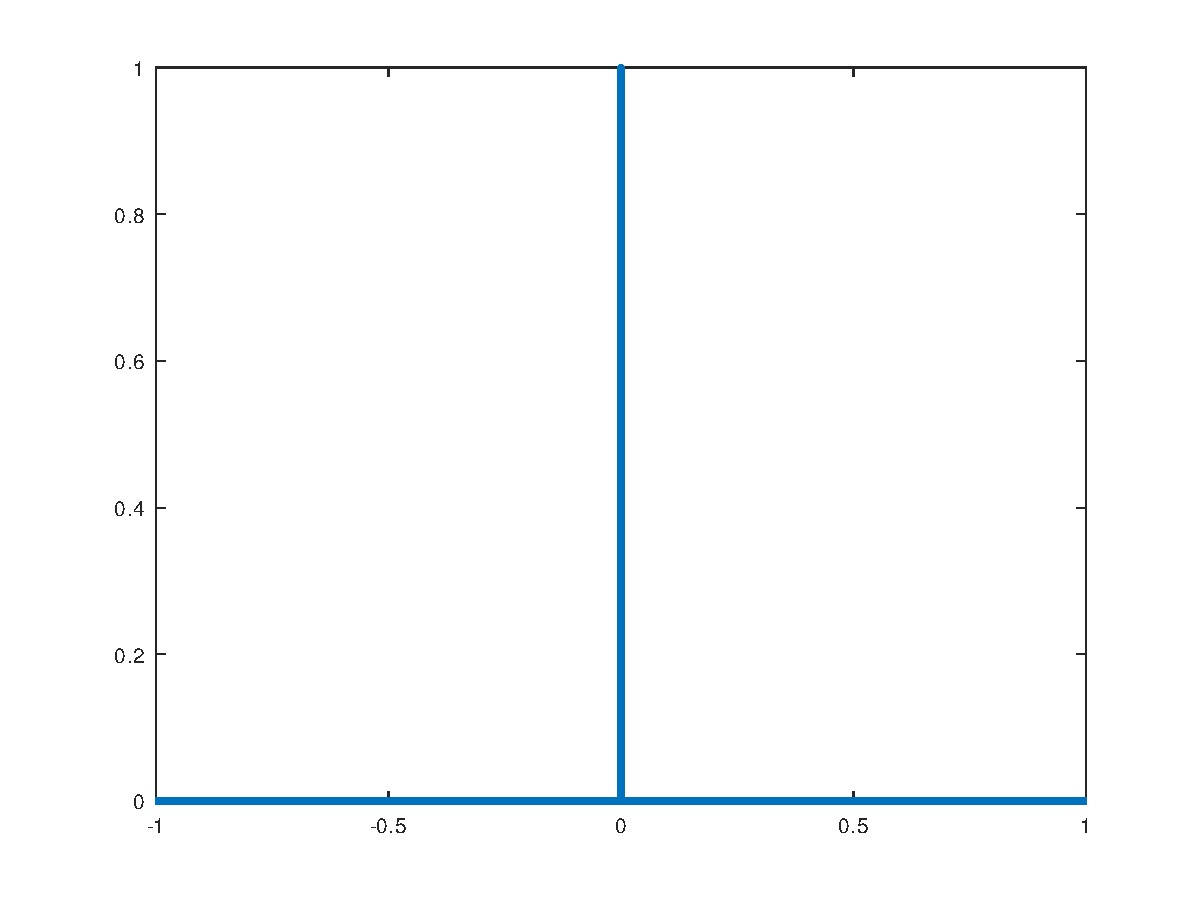
\includegraphics[
    width=\textwidth
    ]{papers/sgwt/images/dirac/dirac_delta.pdf}
    \vspace{-0pt}
    \caption{Darstellung eines Dirac-Stoss $\delta(x)$ mit maximal Wert $1$. 
        \label{fig:sgwt:gft:dirac}}
    \end{minipage}
    ~
    \begin{minipage}[b]{0.49\textwidth}
    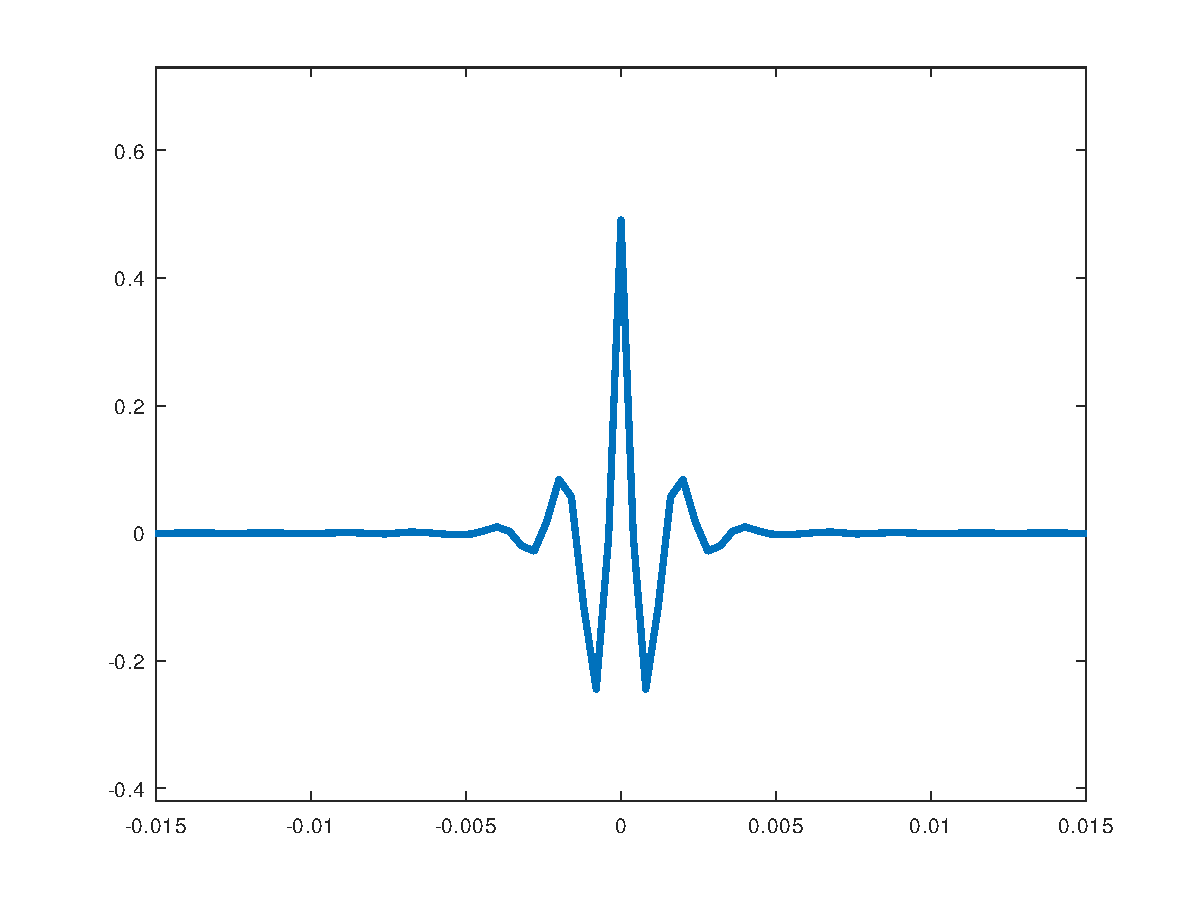
\includegraphics[
    width=\textwidth
    ]{papers/sgwt/images/dirac/dirac_g_igft.pdf}
    \vspace{-0pt}
    \caption{Fourier Transformation des Dirac-Stosses $\hat{\delta(x)}$ 
        aus~\cref{fig:sgwt:gft:dirac}.\label{fig:sgwt:gft:igft}}
    \end{minipage}
    ~
    \begin{minipage}[b]{0.49\textwidth}
    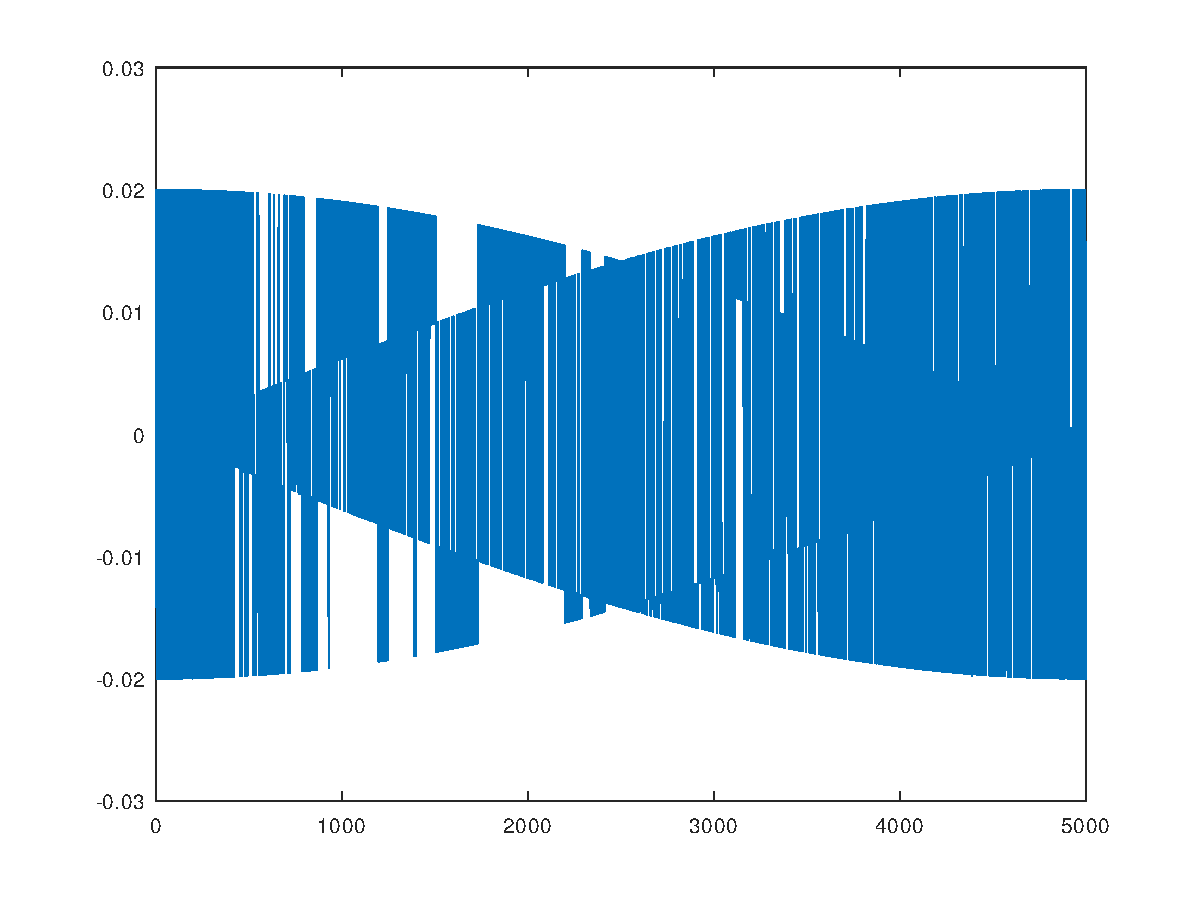
\includegraphics[
    width=\textwidth
    ]{papers/sgwt/images/dirac/dirac_gft.pdf}
    \vspace{-0pt}
    \caption{Fourier Transformation des Dirac-Stosses $\hat{\delta(x)}$ 
        aus~\cref{fig:sgwt:gft:dirac}.\label{fig:sgwt:gft:gft}}
    \end{minipage}
    ~
    \begin{minipage}[b]{0.49\textwidth}
    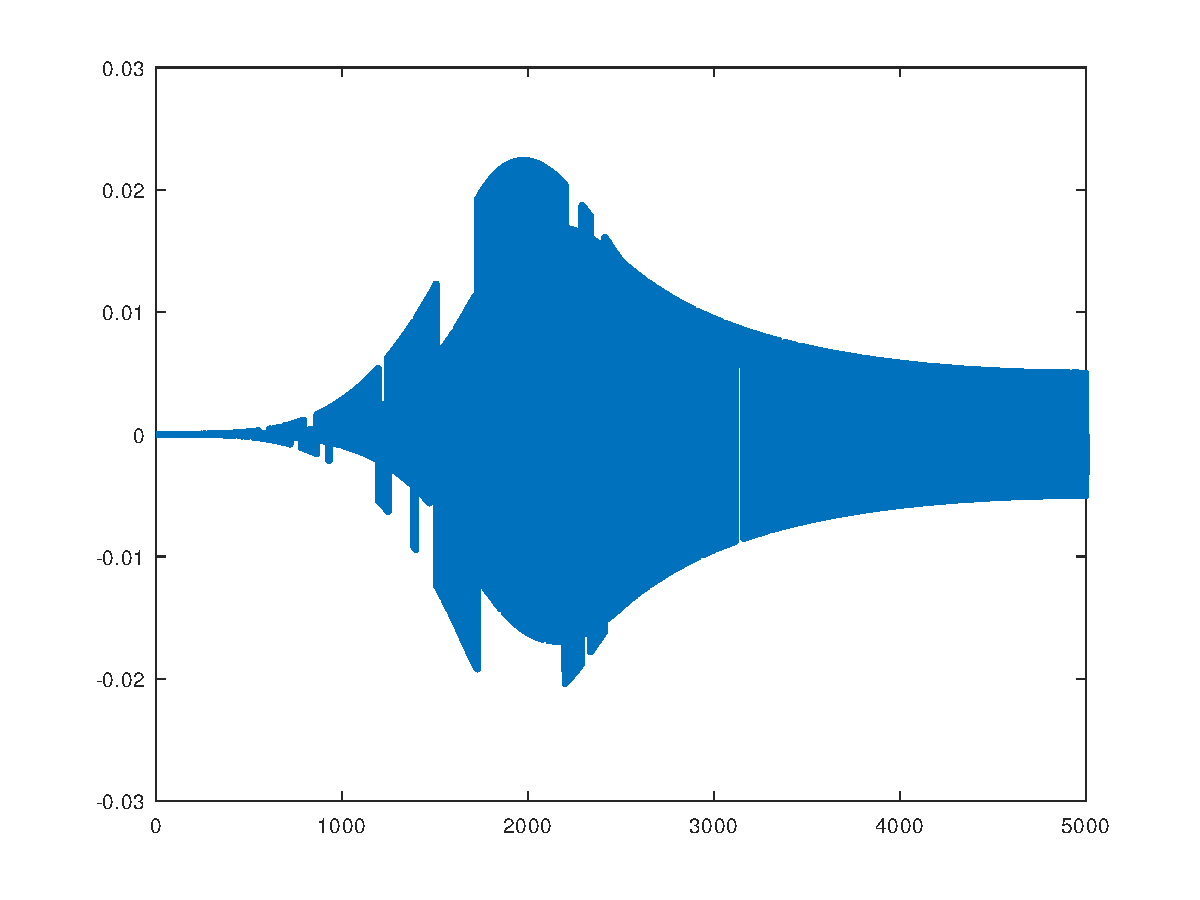
\includegraphics[
    width=\textwidth
    ]{papers/sgwt/images/dirac/dirac_g_gft.pdf}
    \vspace{-0pt}
    \caption{Fourier Transformation des Dirac-Stosses $\hat{\delta(x)}$ 
        aus~\cref{fig:sgwt:gft:dirac}.\label{fig:sgwt:gft:ggft}}
    \end{minipage}
\end{figure}
Wenn wir davon die Fourier Transformation berechnen, zu sehen 
in~\cref{fig:sgwt:gft:fftdirac}, stellen wir fest, das nicht nur alle 
Frequenzen vorhanden sondern auch alle gleich stark vorhanden sind. Die 
Fouriertransformierte $\hat{\delta}$ ist somit vollst\"andig delokalisiert.

$g(\lambda)\cdot\hat{\delta}(\lambda)$

\begin{figure}
    \centering
    \begin{minipage}[b]{0.49\textwidth}
    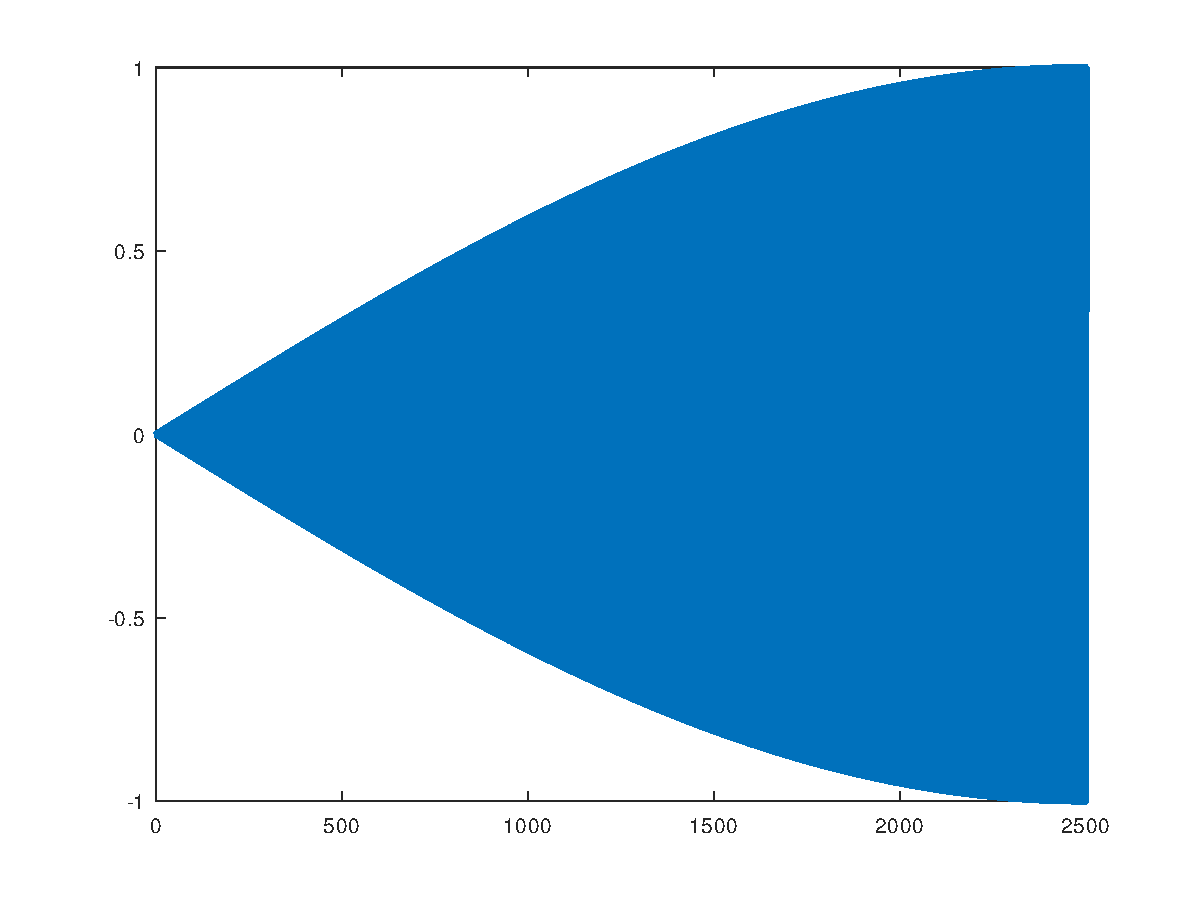
\includegraphics[
    width=\textwidth
    ]{papers/sgwt/images/dirac/dirac_fft_imag.pdf}
    \vspace{-0pt}
    \caption{Darstellung eines Dirac-Stoss $\delta(x)$ mit maximal Wert $1$. 
        \label{fig:sgwt:gft:dirac}}
    \end{minipage}
    ~
    \begin{minipage}[b]{0.49\textwidth}
    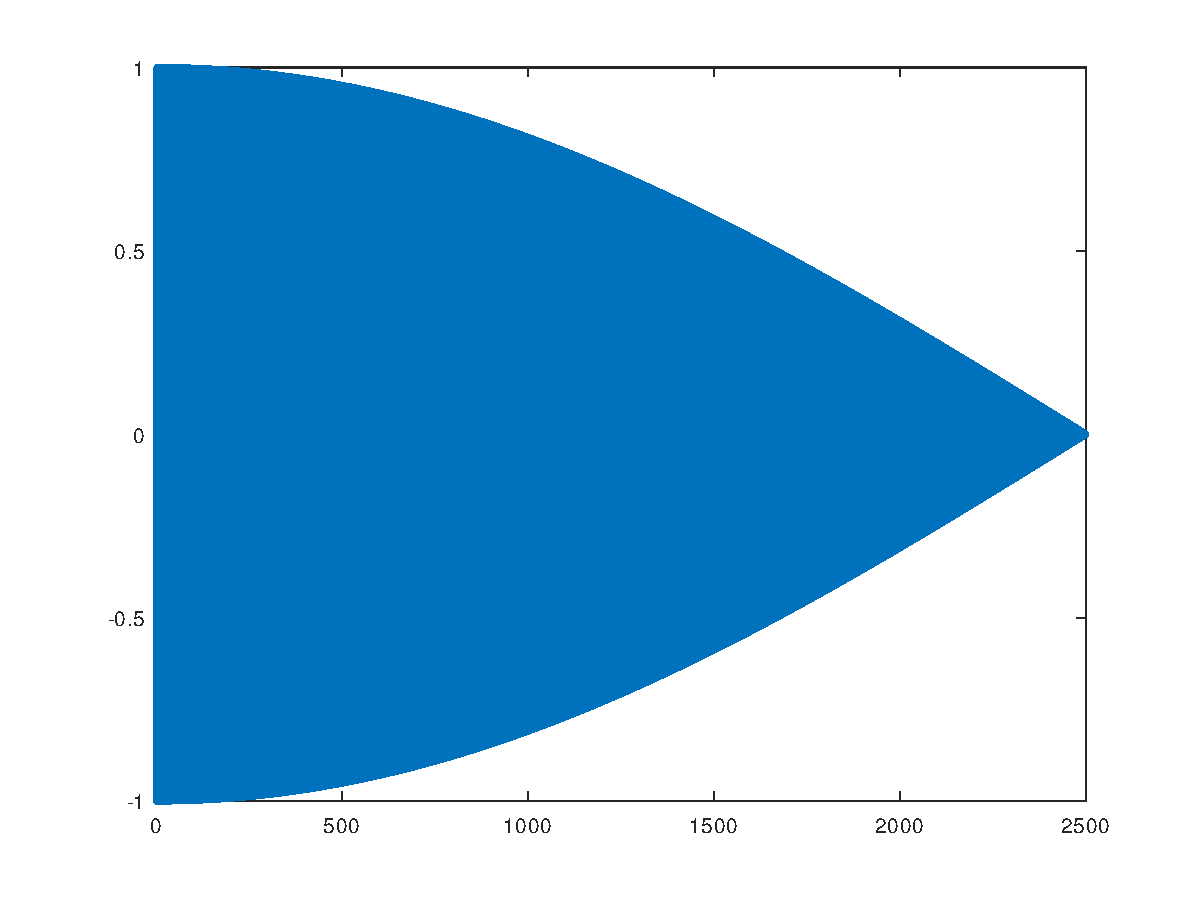
\includegraphics[
    width=\textwidth
    ]{papers/sgwt/images/dirac/dirac_fft_real.pdf}
    \vspace{-0pt}
    \caption{Fourier Transformation des Dirac-Stosses $\hat{\delta(x)}$ 
        aus~\cref{fig:sgwt:gft:dirac}.\label{fig:sgwt:gft:igft}}
    \end{minipage}
\end{figure}

\begin{figure}
    \centering
    \begin{minipage}[b]{0.49\textwidth}
    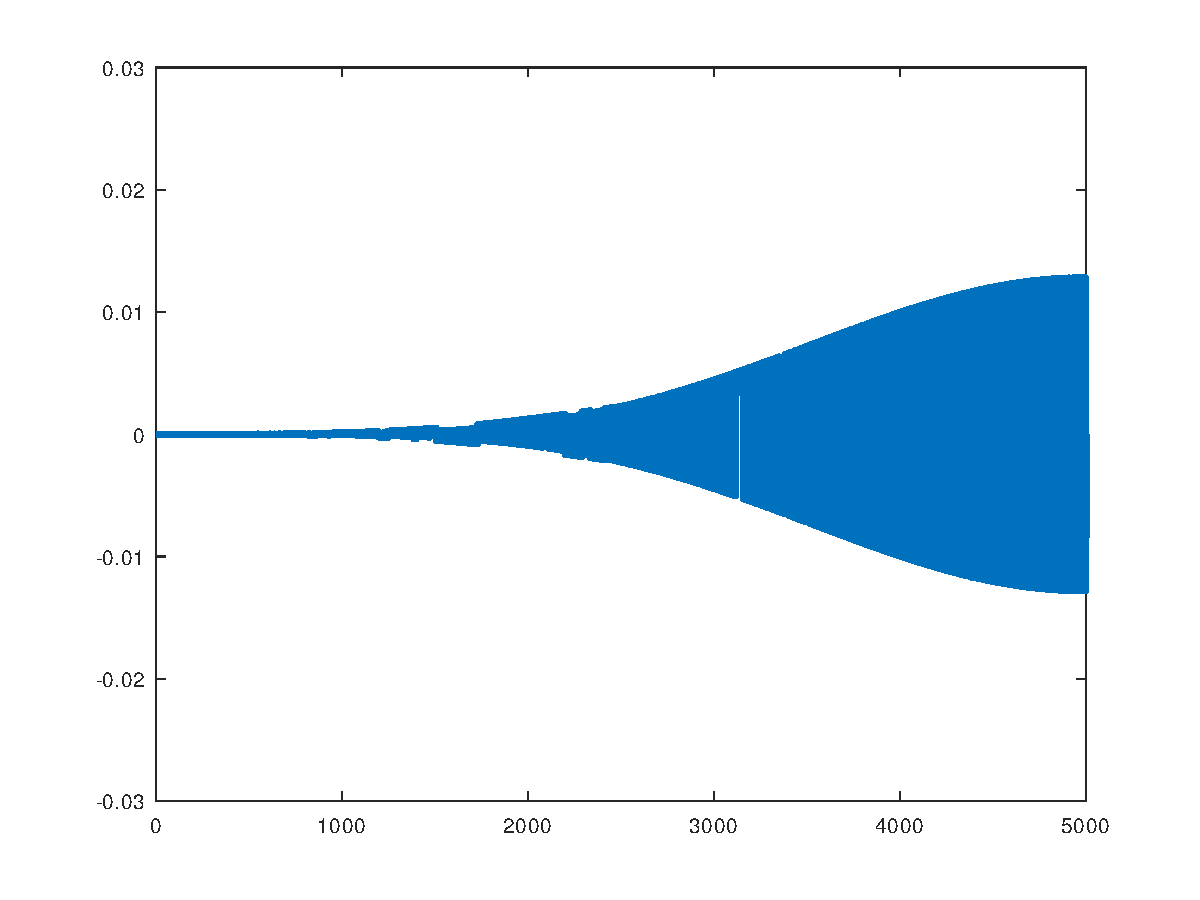
\includegraphics[
    width=\textwidth
    ]{papers/sgwt/images/dirac/dirac_gt1_gft.pdf}
    \vspace{-0pt}
    \caption{Darstellung eines Dirac-Stoss $\delta(x)$ mit maximal Wert $1$. 
        \label{fig:sgwt:gft:dirac}}
    \end{minipage}
    ~
    \begin{minipage}[b]{0.49\textwidth}
    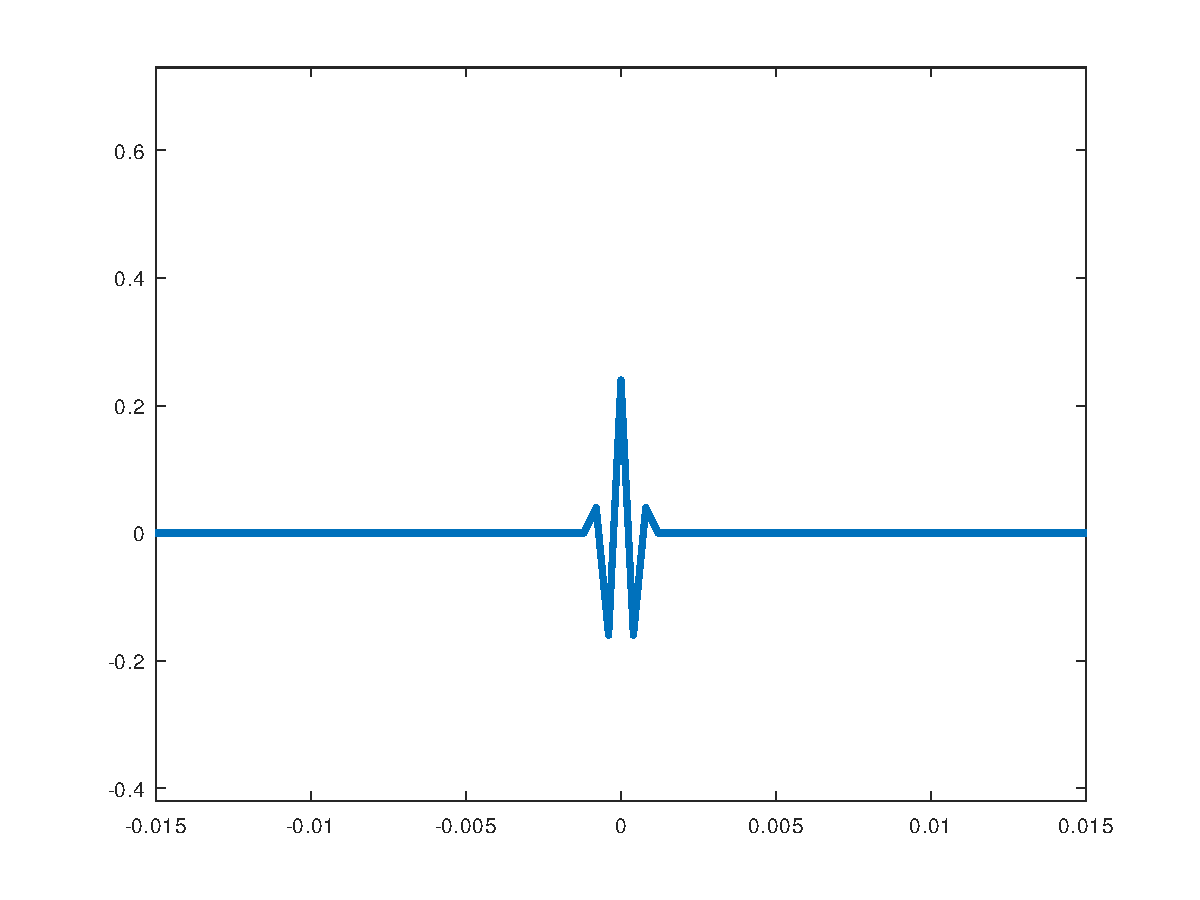
\includegraphics[
    width=\textwidth
    ]{papers/sgwt/images/dirac/dirac_gt1_igft.pdf}
    \vspace{-0pt}
    \caption{Fourier Transformation des Dirac-Stosses $\hat{\delta(x)}$ 
        aus~\cref{fig:sgwt:gft:dirac}.\label{fig:sgwt:gft:igft}}
    \end{minipage}
    ~
    \begin{minipage}[b]{0.49\textwidth}
    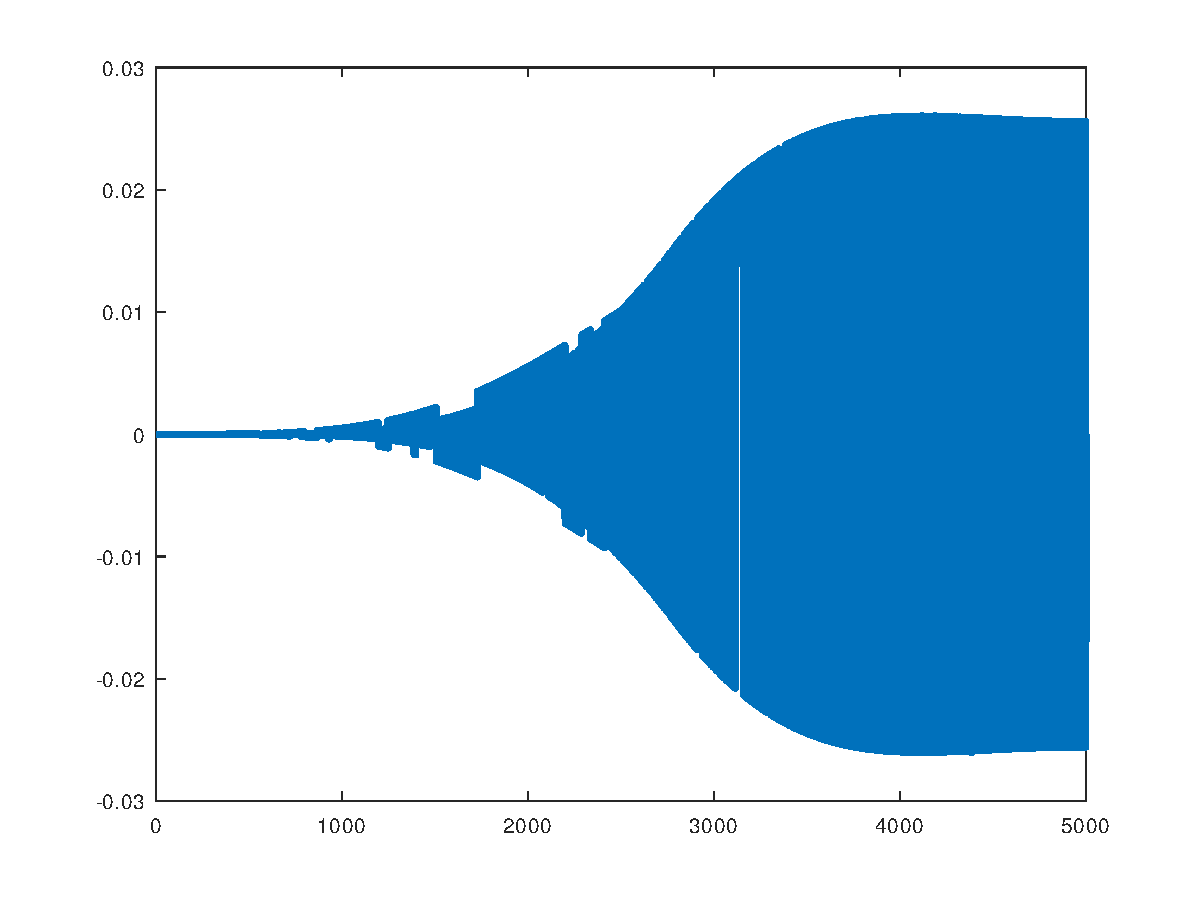
\includegraphics[
    width=\textwidth
    ]{papers/sgwt/images/dirac/dirac_gt2_gft.pdf}
    \vspace{-0pt}
    \caption{Fourier Transformation des Dirac-Stosses $\hat{\delta(x)}$ 
        aus~\cref{fig:sgwt:gft:dirac}.\label{fig:sgwt:gft:gft}}
    \end{minipage}
    ~
    \begin{minipage}[b]{0.49\textwidth}
    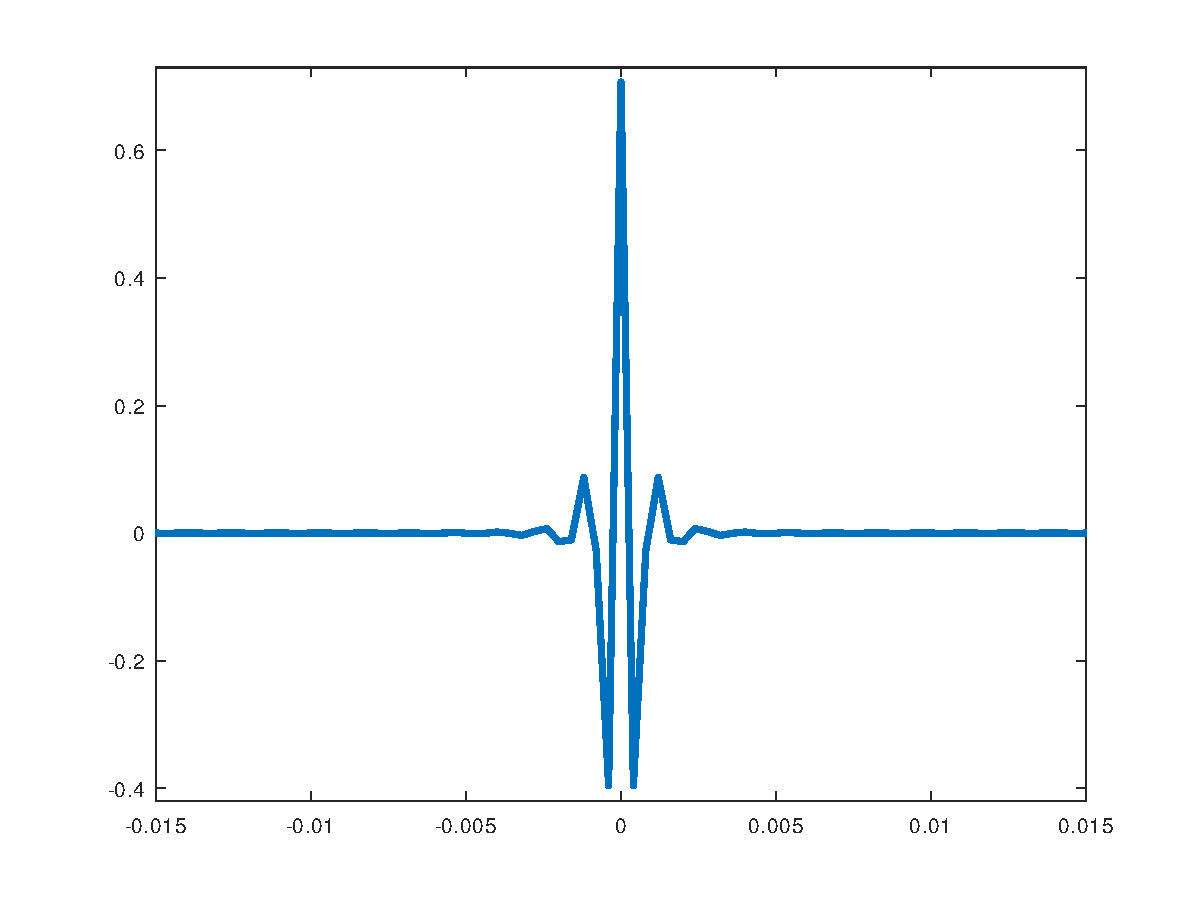
\includegraphics[
    width=\textwidth
    ]{papers/sgwt/images/dirac/dirac_gt2_igft.pdf}
    \vspace{-0pt}
    \caption{Fourier Transformation des Dirac-Stosses $\hat{\delta(x)}$ 
        aus~\cref{fig:sgwt:gft:dirac}.\label{fig:sgwt:gft:ggft}}
    \end{minipage}
    ~
    \begin{minipage}[b]{0.49\textwidth}
    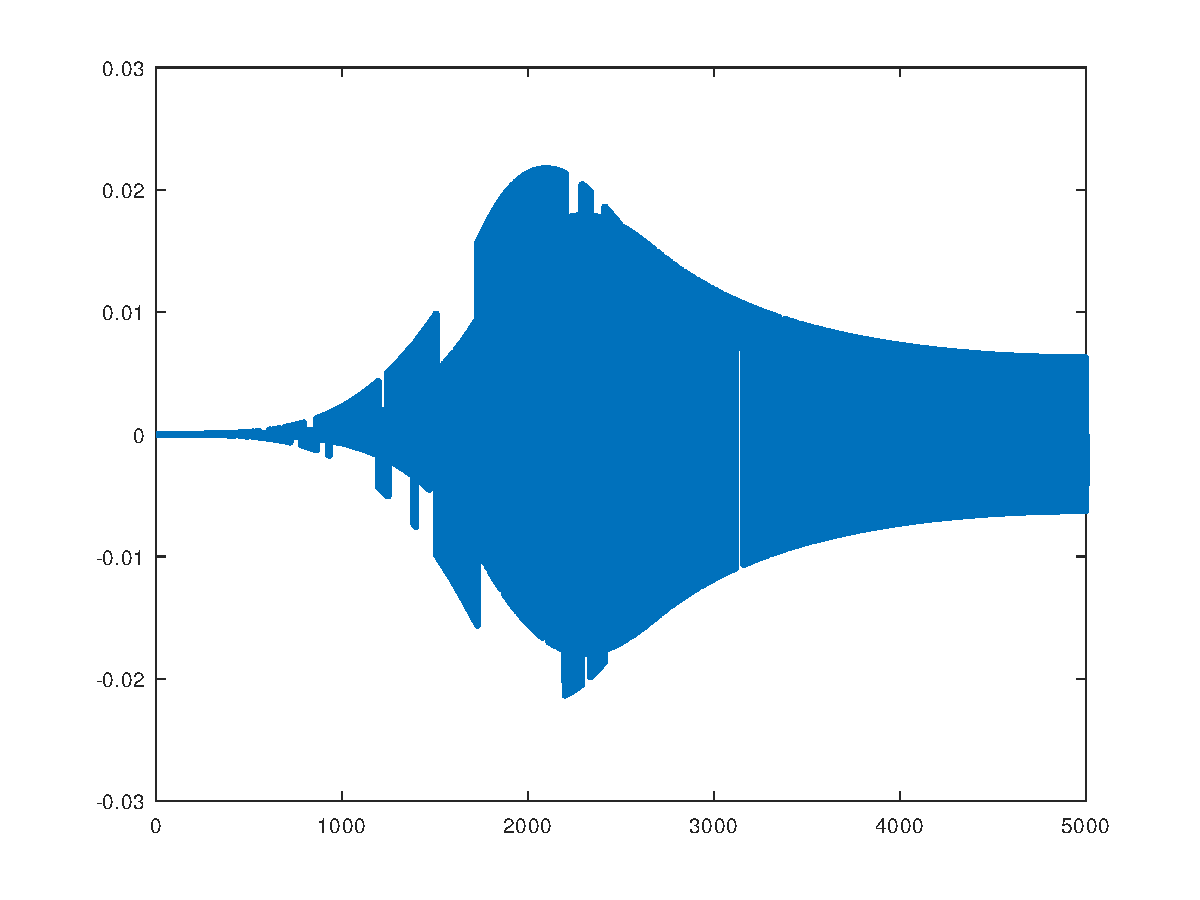
\includegraphics[
    width=\textwidth
    ]{papers/sgwt/images/dirac/dirac_gt3_gft.pdf}
    \vspace{-0pt}
    \caption{Fourier Transformation des Dirac-Stosses $\hat{\delta(x)}$ 
        aus~\cref{fig:sgwt:gft:dirac}.\label{fig:sgwt:gft:ggft}}
    \end{minipage}
    ~
    \begin{minipage}[b]{0.49\textwidth}
    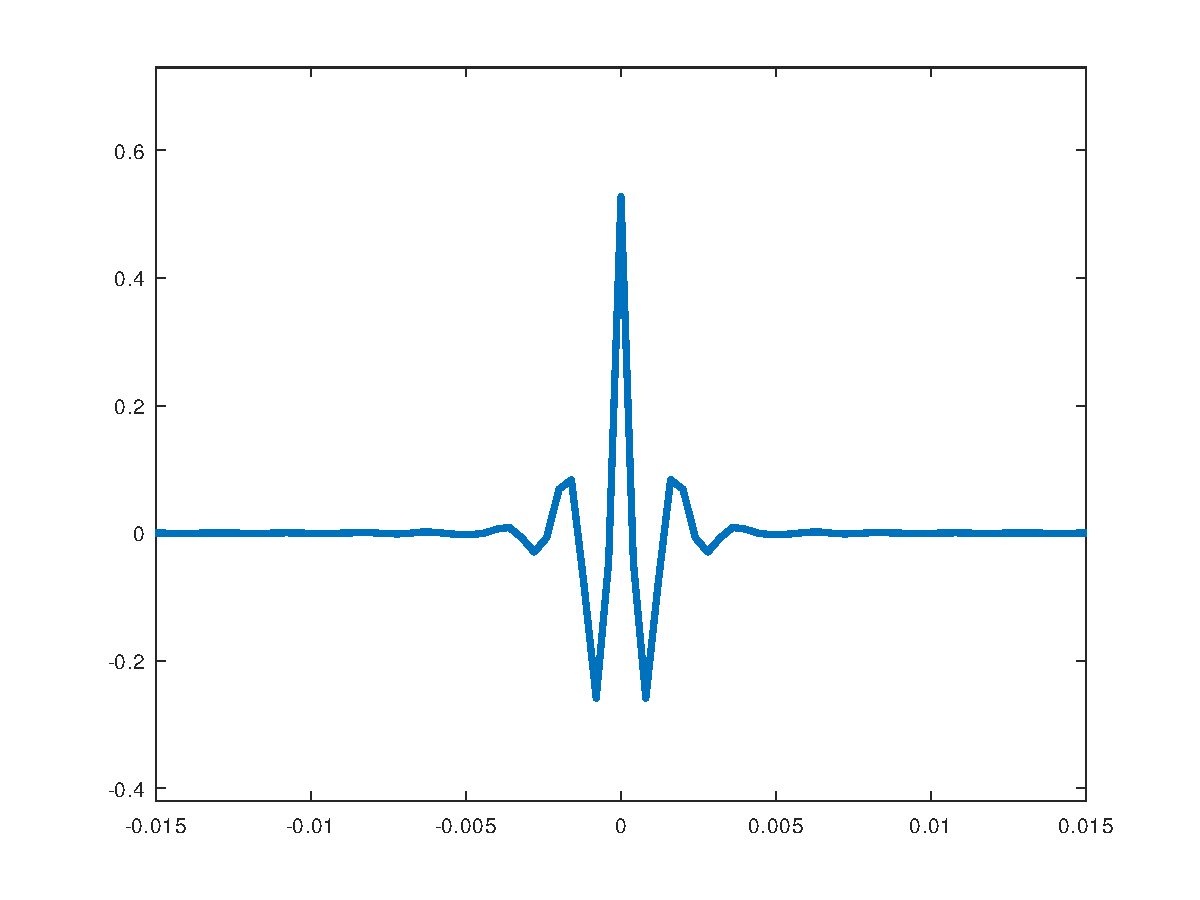
\includegraphics[
    width=\textwidth
    ]{papers/sgwt/images/dirac/dirac_gt3_igft.pdf}
    \vspace{-0pt}
    \caption{Fourier Transformation des Dirac-Stosses $\hat{\delta(x)}$ 
        aus~\cref{fig:sgwt:gft:dirac}.\label{fig:sgwt:gft:ggft}}
    \end{minipage}
\end{figure}



\begin{figure}
    \centering
    \begin{minipage}[b]{0.49\textwidth}
    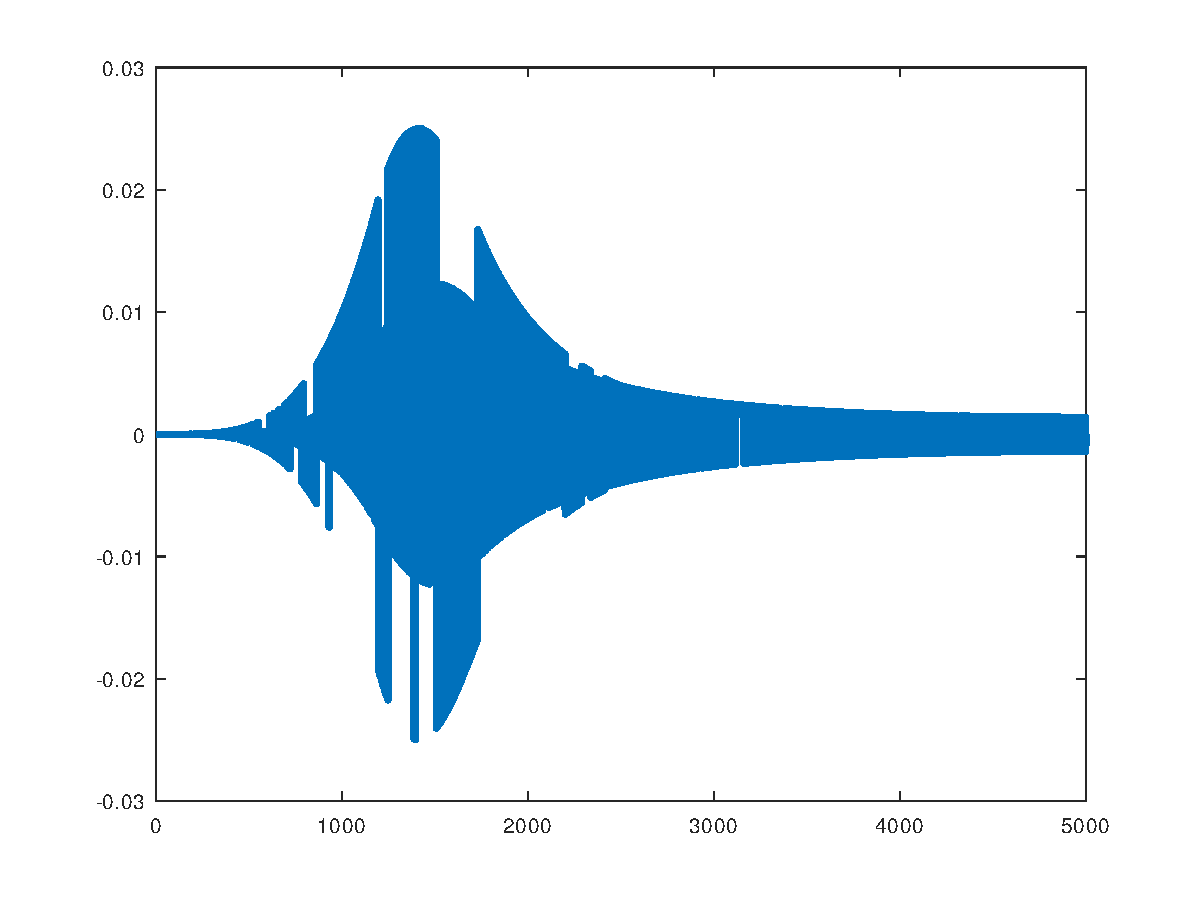
\includegraphics[
    width=\textwidth
    ]{papers/sgwt/images/dirac/dirac_gt4_gft.pdf}
    \vspace{-0pt}
    \caption{Darstellung eines Dirac-Stoss $\delta(x)$ mit maximal Wert $1$. 
        \label{fig:sgwt:gft:dirac}}
    \end{minipage}
    ~
    \begin{minipage}[b]{0.49\textwidth}
    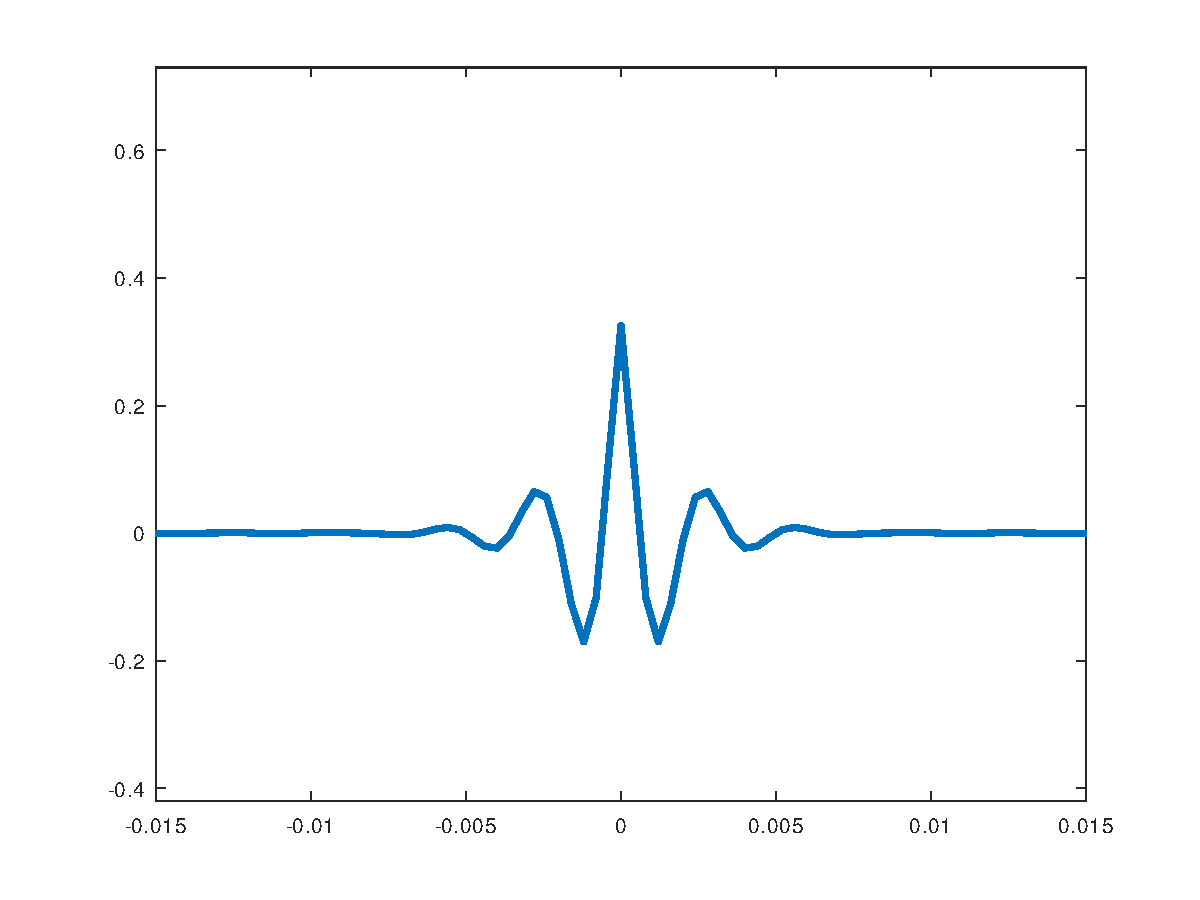
\includegraphics[
    width=\textwidth
    ]{papers/sgwt/images/dirac/dirac_gt4_igft.pdf}
    \vspace{-0pt}
    \caption{Fourier Transformation des Dirac-Stosses $\hat{\delta(x)}$ 
        aus~\cref{fig:sgwt:gft:dirac}.\label{fig:sgwt:gft:igft}}
    \end{minipage}
    ~
    \begin{minipage}[b]{0.49\textwidth}
    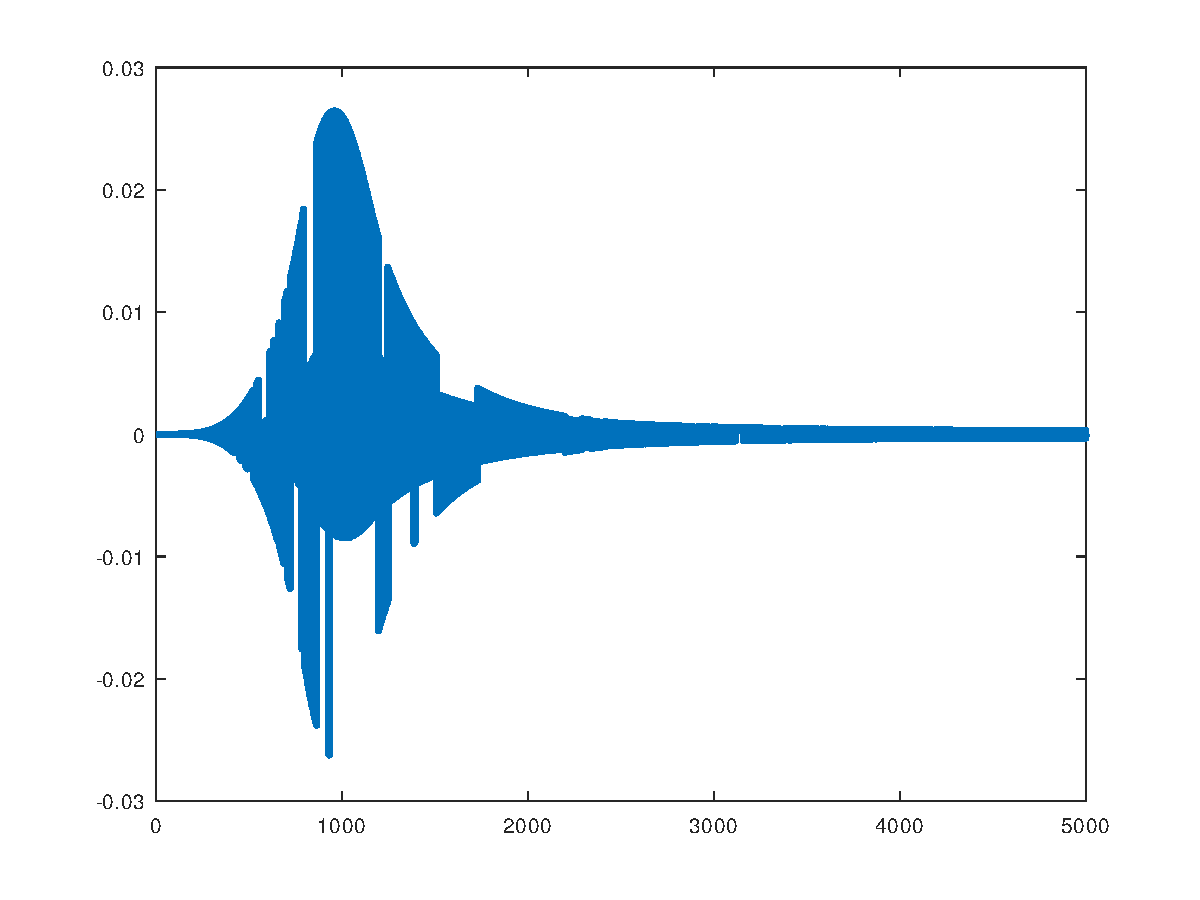
\includegraphics[
    width=\textwidth
    ]{papers/sgwt/images/dirac/dirac_gt5_gft.pdf}
    \vspace{-0pt}
    \caption{Fourier Transformation des Dirac-Stosses $\hat{\delta(x)}$ 
        aus~\cref{fig:sgwt:gft:dirac}.\label{fig:sgwt:gft:gft}}
    \end{minipage}
    ~
    \begin{minipage}[b]{0.49\textwidth}
    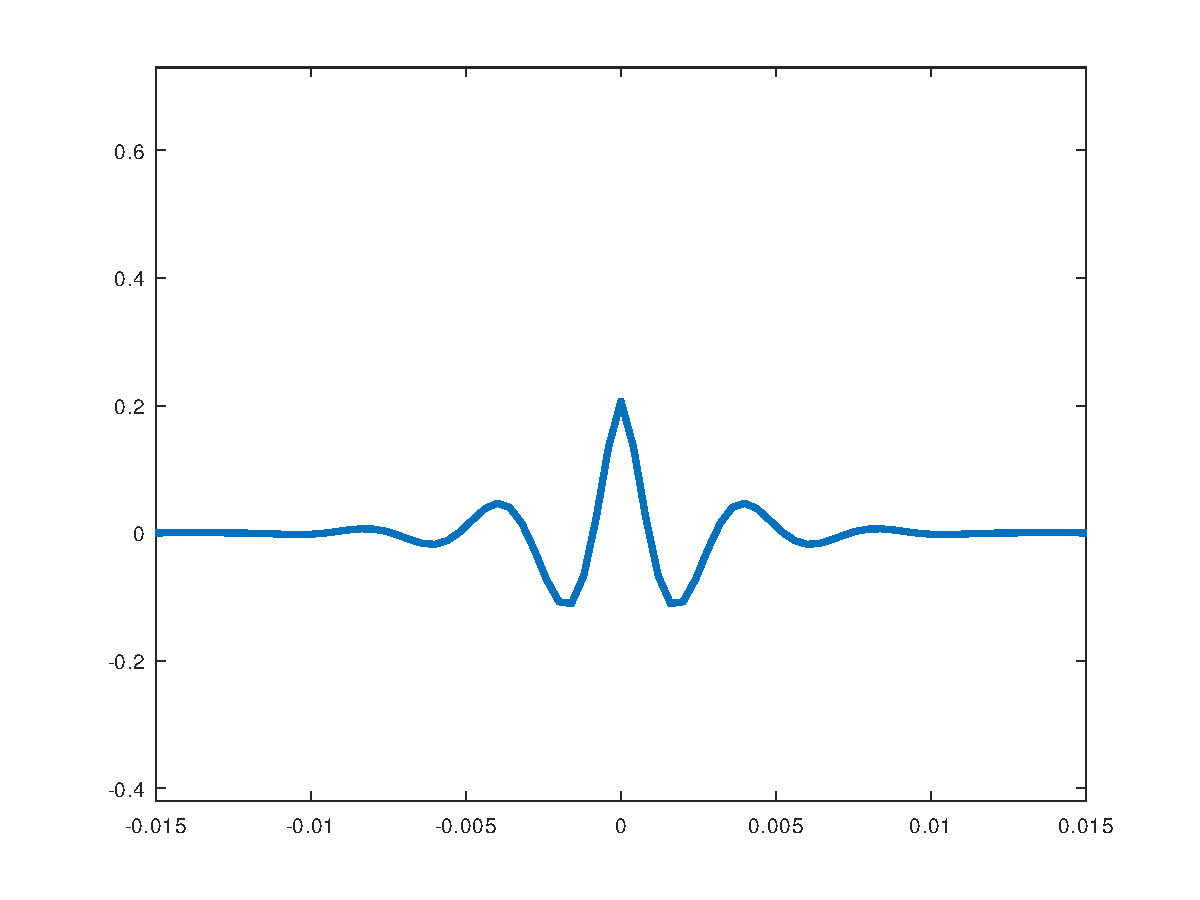
\includegraphics[
    width=\textwidth
    ]{papers/sgwt/images/dirac/dirac_gt5_igft.pdf}
    \vspace{-0pt}
    \caption{Fourier Transformation des Dirac-Stosses $\hat{\delta(x)}$ 
        aus~\cref{fig:sgwt:gft:dirac}.\label{fig:sgwt:gft:ggft}}
    \end{minipage}
    ~
    \begin{minipage}[b]{0.49\textwidth}
    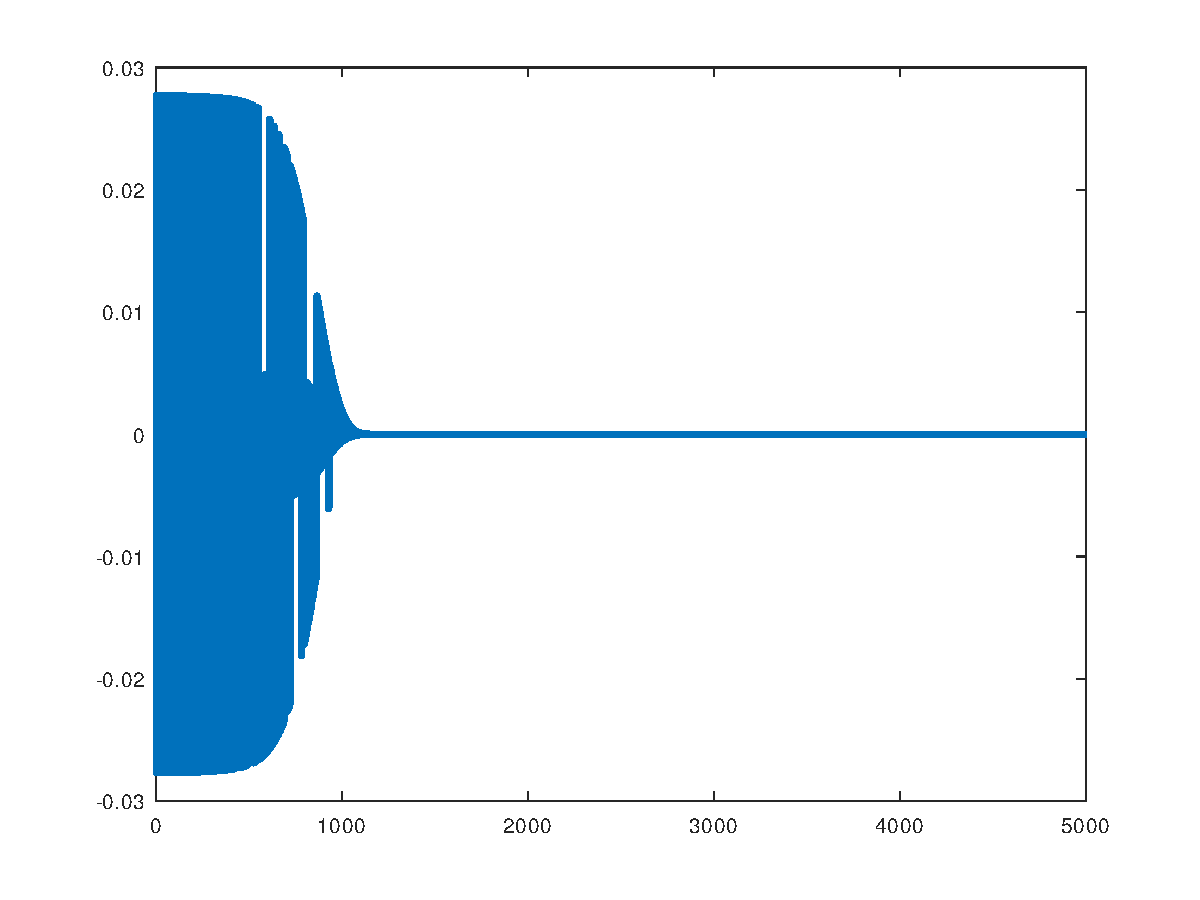
\includegraphics[
    width=\textwidth
    ]{papers/sgwt/images/dirac/dirac_h_gft.pdf}
    \vspace{-0pt}
    \caption{Fourier Transformation des Dirac-Stosses $\hat{\delta(x)}$ 
        aus~\cref{fig:sgwt:gft:dirac}.\label{fig:sgwt:gft:ggft}}
    \end{minipage}
    ~
    \begin{minipage}[b]{0.49\textwidth}
    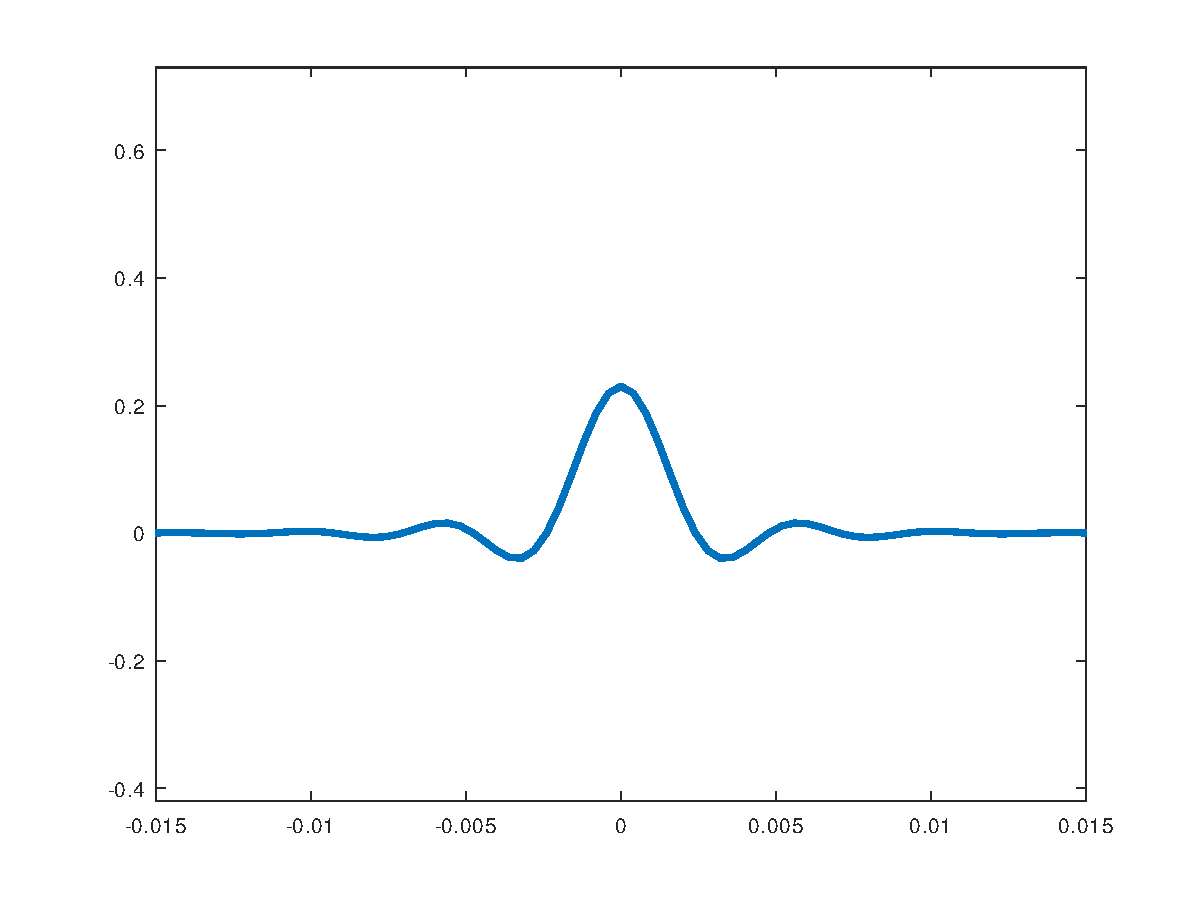
\includegraphics[
    width=\textwidth
    ]{papers/sgwt/images/dirac/dirac_h_igft.pdf}
    \vspace{-0pt}
    \caption{Fourier Transformation des Dirac-Stosses $\hat{\delta(x)}$ 
        aus~\cref{fig:sgwt:gft:dirac}.\label{fig:sgwt:gft:ggft}}
    \end{minipage}
\end{figure}

\begin{figure}
    \centering
    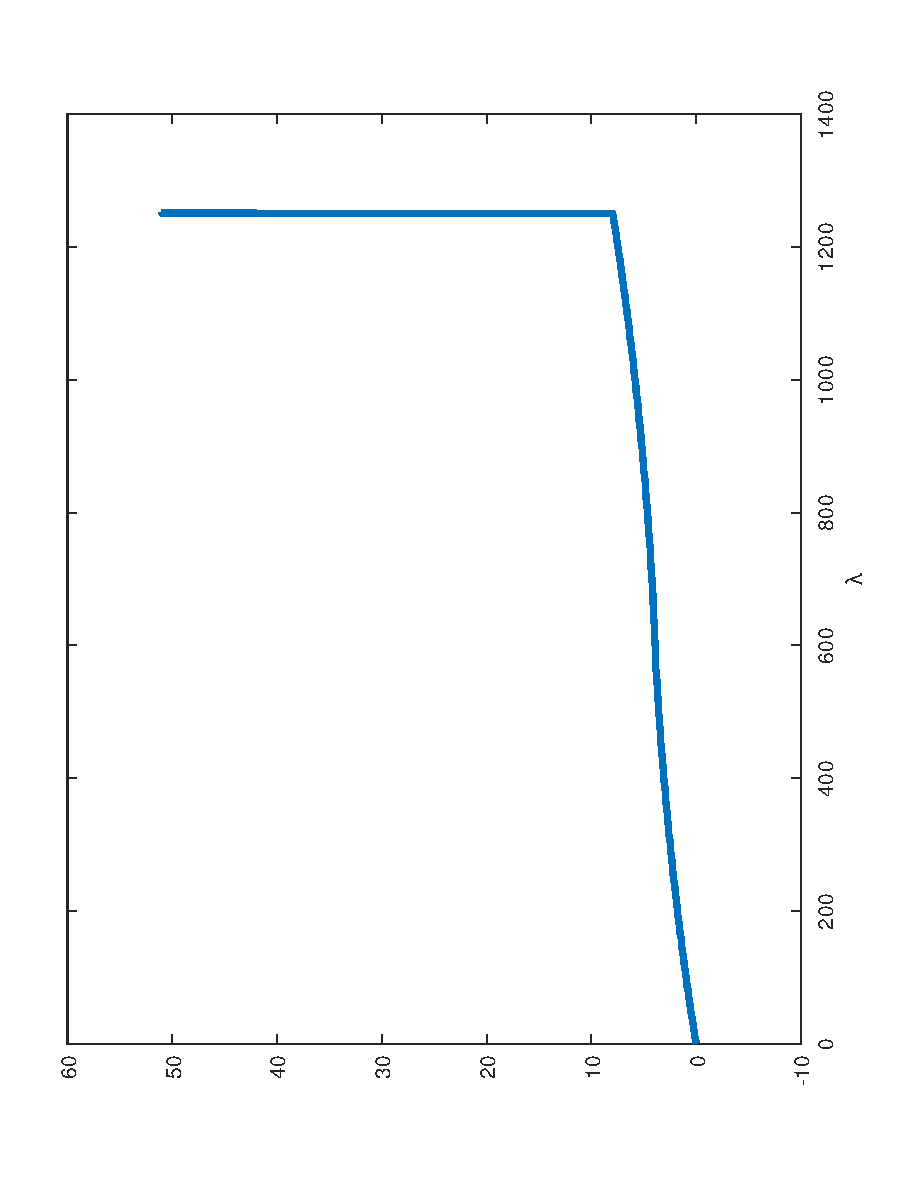
\includegraphics[
    angle=-90,
    origin=c,
    scale=0.6
    ]{papers/sgwt/images/wavelets/lambda.pdf}
    \vspace{-50pt}
    \caption{Eigenwerte $\lambda$ eines Kugelgraphen mit 1252 Knoten. 
    \label{fig:sgwt:wavelets:sphere:lambda}}
\end{figure}

\begin{figure}
    \begin{minipage}[b]{0.49\textwidth}
        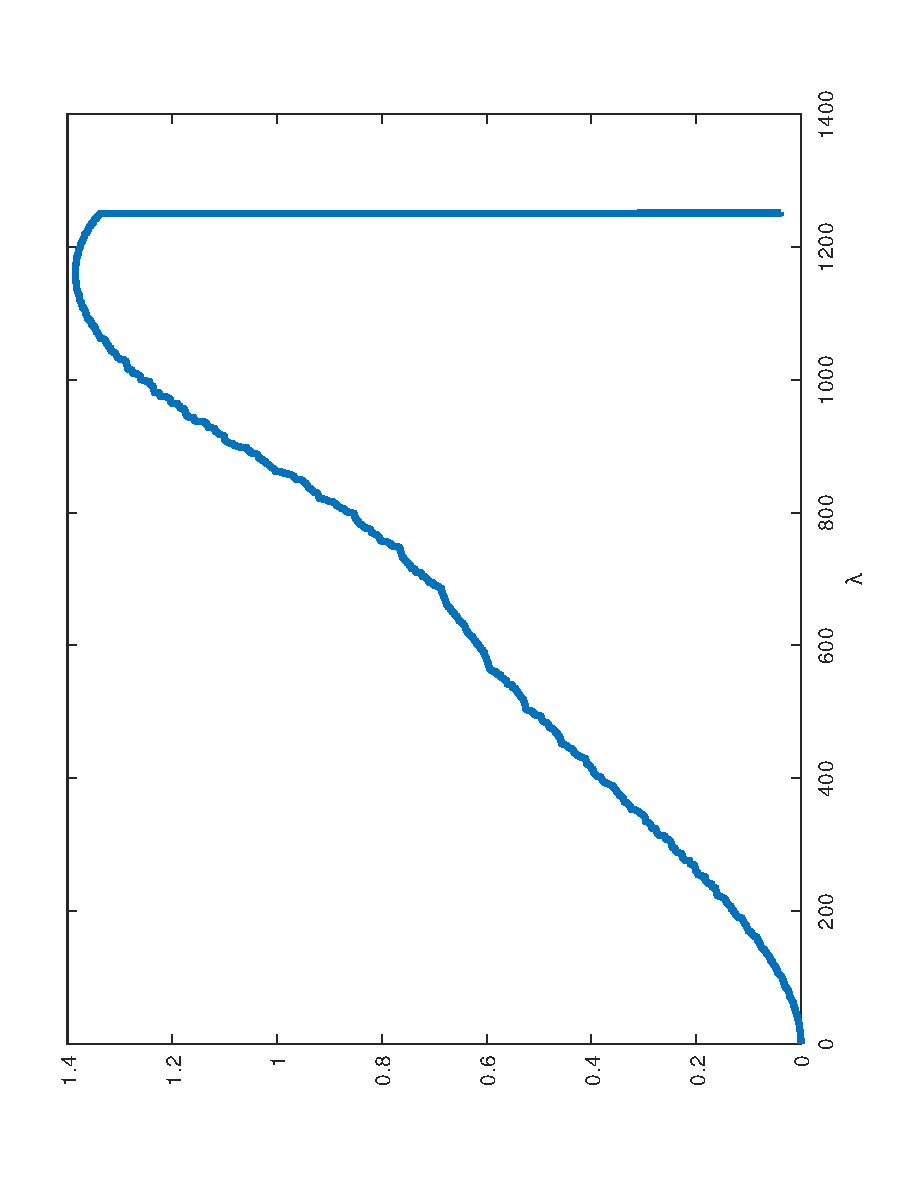
\includegraphics[
        angle=-90,
        origin=c,
        width=\textwidth]{papers/sgwt/images/wavelets/gt1.pdf}
        \vspace{-45pt}
        \caption{Die Kernelfunktion $g(t_1\lambda)$ eines Kugelgraphen mit 1252 
        Knoten und $t_1 = 0.2$.}
        \label{fig:sgwt:wavelets:sphere:gt1}
    \end{minipage}
    ~
    \begin{minipage}[b]{0.49\textwidth}
        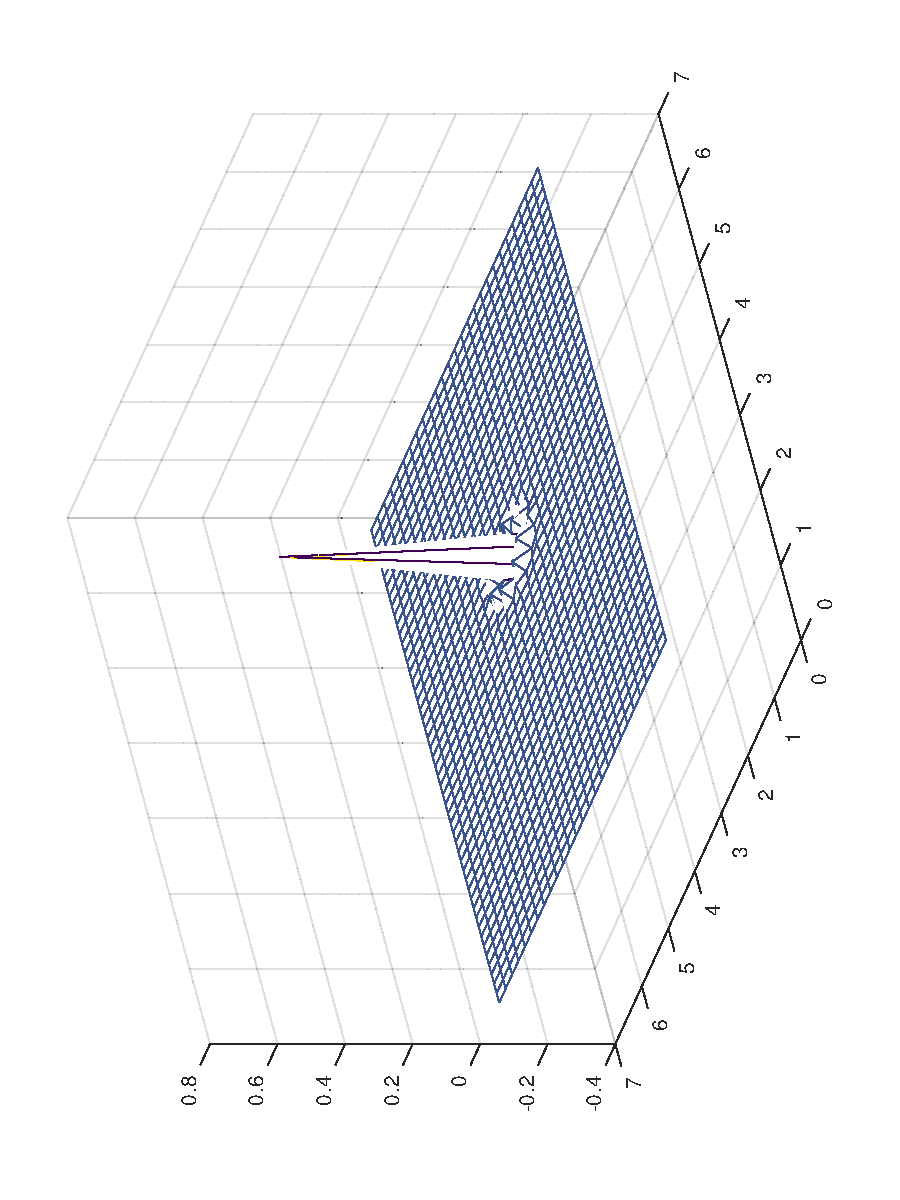
\includegraphics[
        angle=-90,
        origin=c,
        width=\textwidth]{papers/sgwt/images/wavelets/psi_t1_50_25_630_flat.pdf}
        \vspace{-45pt}
        \caption{$\psi_1(v_{630})$-Wavelet eines Kugelgraphen mit 1252 Knoten.}
        \label{fig:sgwt:wavelets:sphere:psi1:flat}
    \end{minipage}
    ~
    \begin{minipage}[b]{\textwidth}
        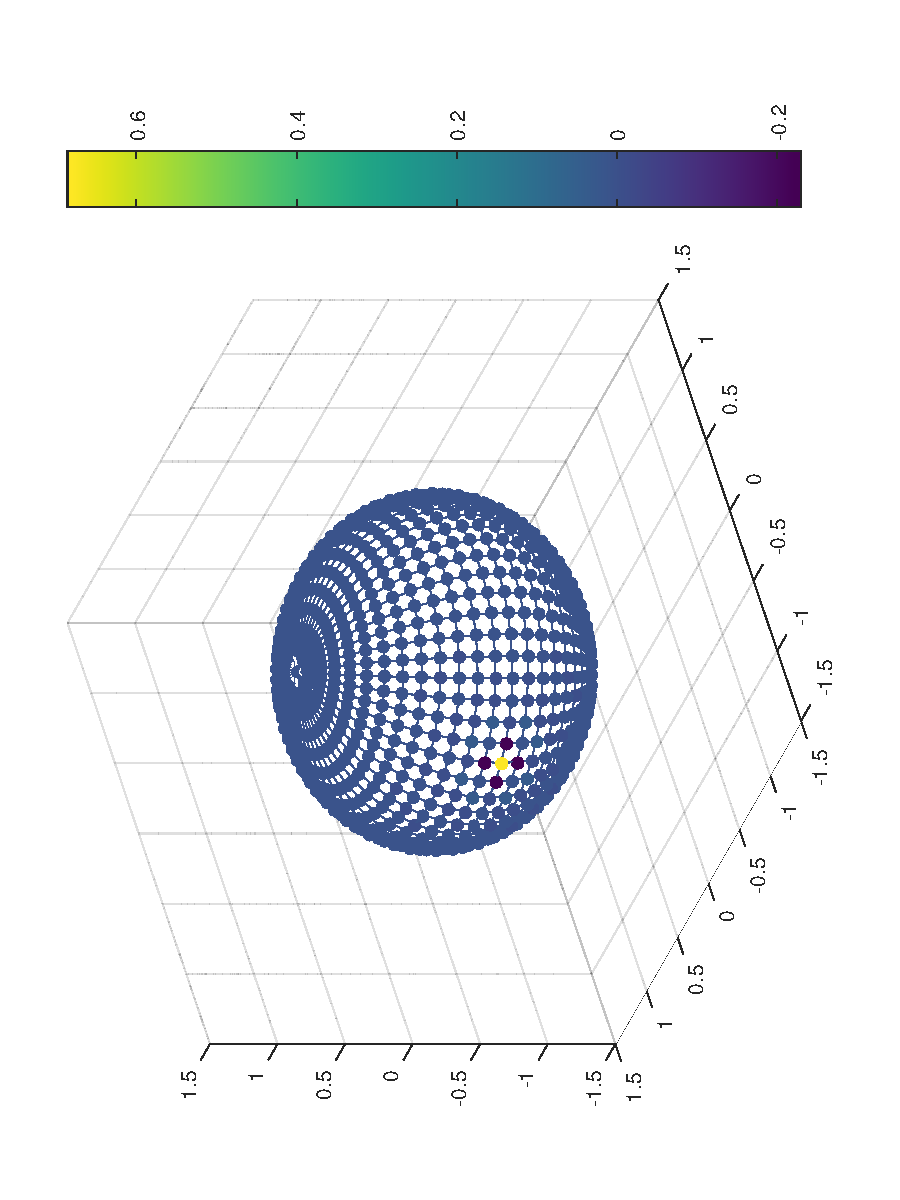
\includegraphics[
        angle=-90,
        origin=c,
        width=\textwidth]{papers/sgwt/images/wavelets/psi_t1_50_25_630.pdf}
        \vspace{-45pt}
        \caption{$\psi_1(v_{630})$-Wavelet eines Kugelgraphen mit 1252 Knoten 
        und $t = 0.42295$.}
        \label{fig:sgwt:wavelets:sphere:psi1}
    \end{minipage}
\end{figure}

\begin{figure}
    \begin{minipage}[b]{0.49\textwidth}
        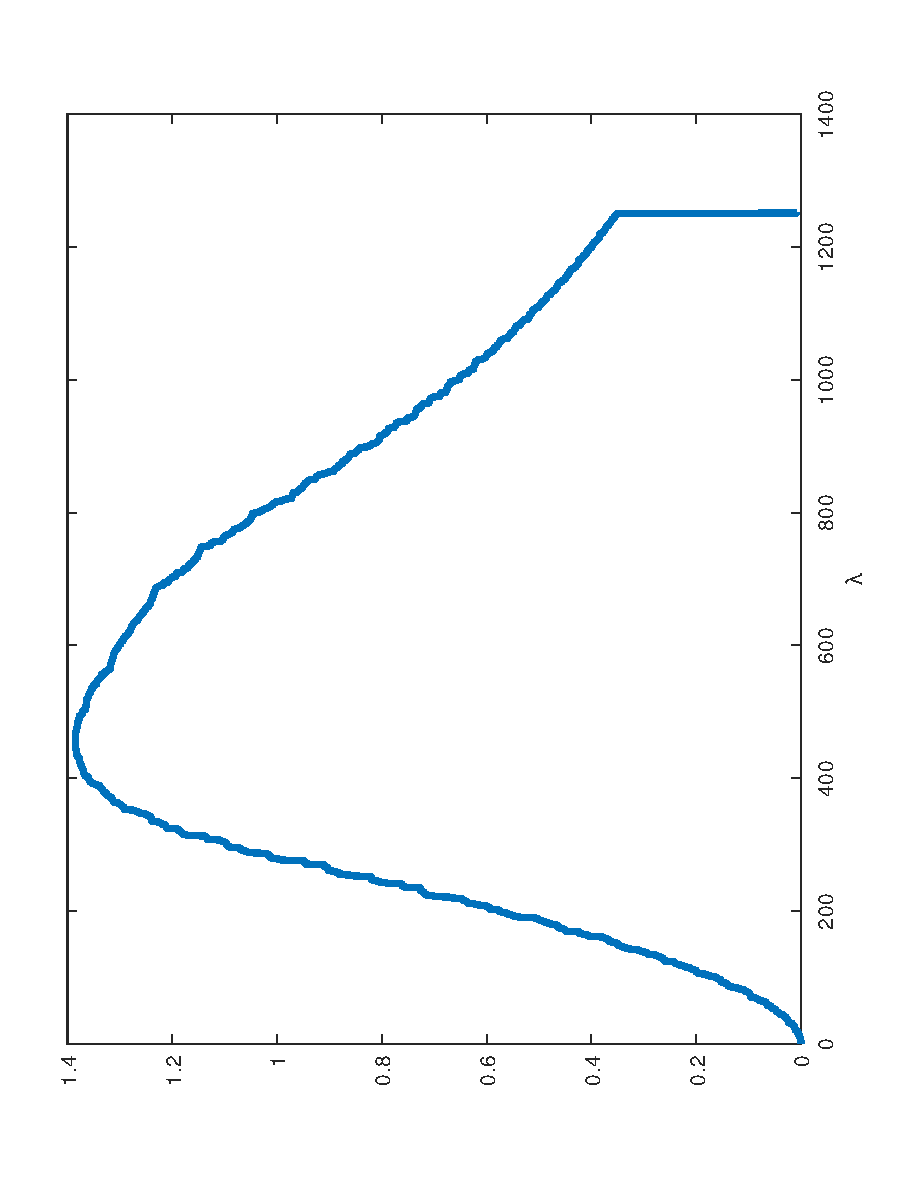
\includegraphics[
        angle=-90,
        origin=c,
        width=\textwidth]{papers/sgwt/images/wavelets/gt2.pdf}
        \vspace{-45pt}
        \caption{Die Kernelfunktion $g(t_2\lambda)$ eines Kugelgraphen mit 1252 
            Knoten und $t_2 = 0.42295$.}
        \label{fig:sgwt:wavelets:sphere:gt2}
    \end{minipage}
    ~
    \begin{minipage}[b]{0.49\textwidth}
        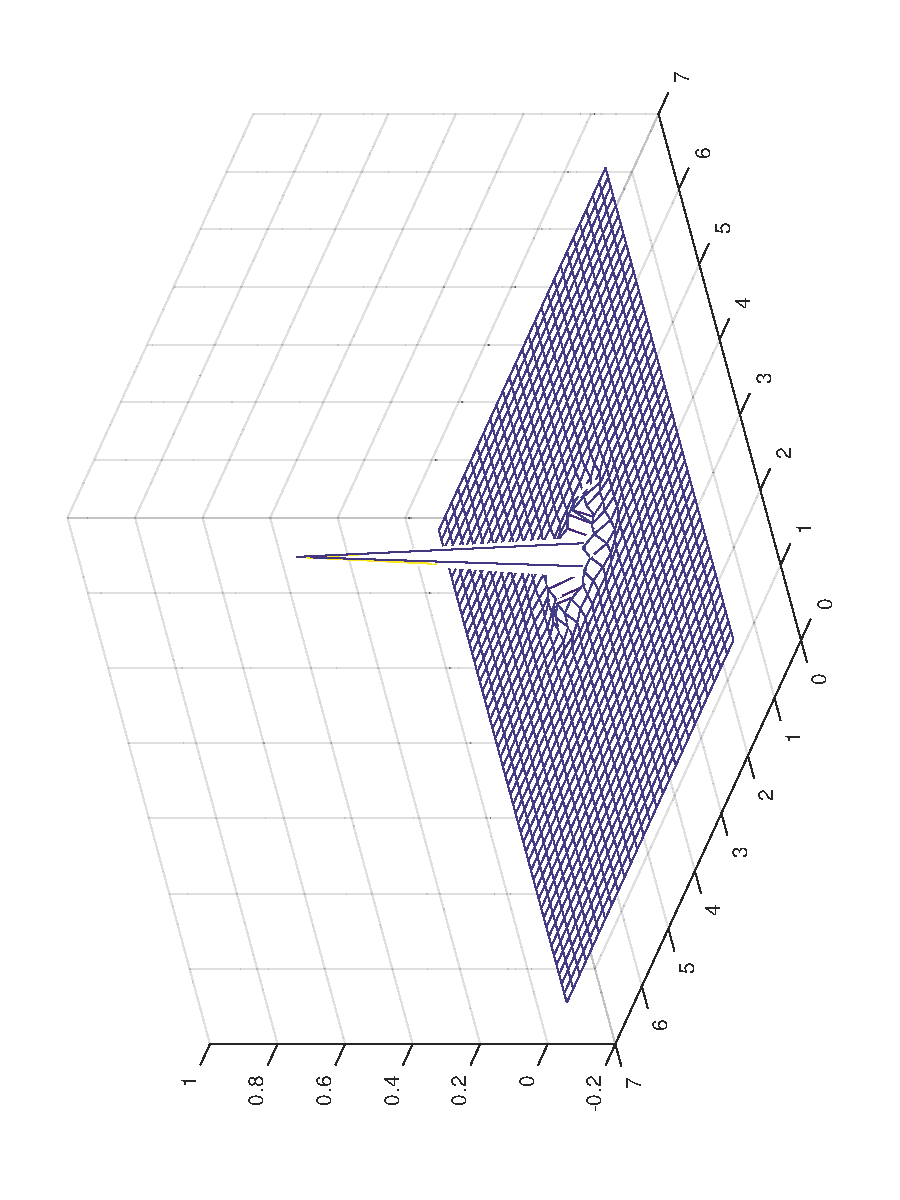
\includegraphics[
        angle=-90,
        origin=c,
        width=\textwidth]{papers/sgwt/images/wavelets/psi_t2_50_25_630_flat.pdf}
        \vspace{-45pt}
        \caption{$\psi_2(v_{630})$-Wavelet eines Kugelgraphen mit 1252 Knoten.}
        \label{fig:sgwt:wavelets:sphere:psi2:flat}
    \end{minipage}
    ~
    \begin{minipage}[b]{\textwidth}
        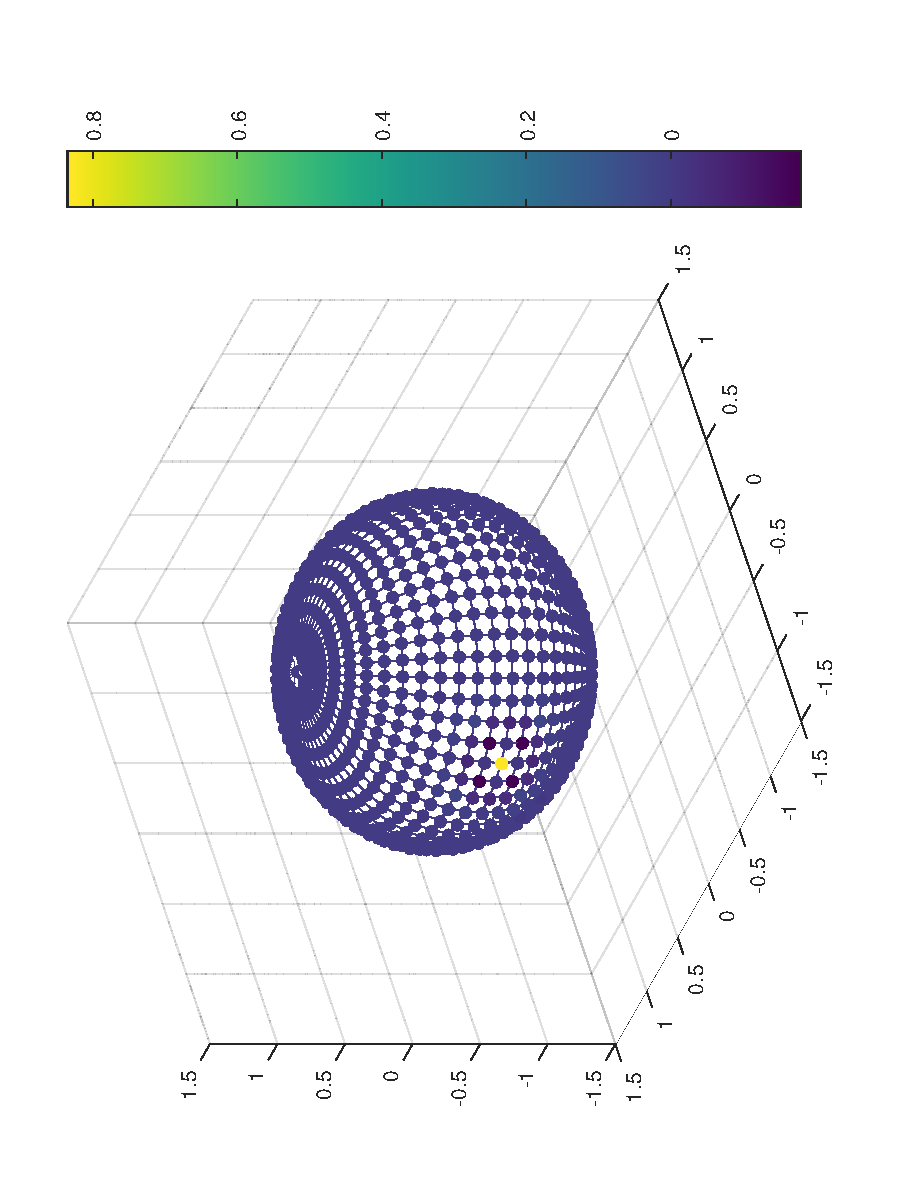
\includegraphics[
        angle=-90,
        origin=c,
        width=\textwidth]{papers/sgwt/images/wavelets/psi_t2_50_25_630.pdf}
        \vspace{-45pt}
        \caption{$\psi_2(v_{630})$-Wavelet eines Kugelgraphen mit 1252 Knoten.}
        \label{fig:sgwt:wavelets:sphere:psi2}
    \end{minipage}
\end{figure}

\begin{figure}
    \begin{minipage}[b]{0.49\textwidth}
        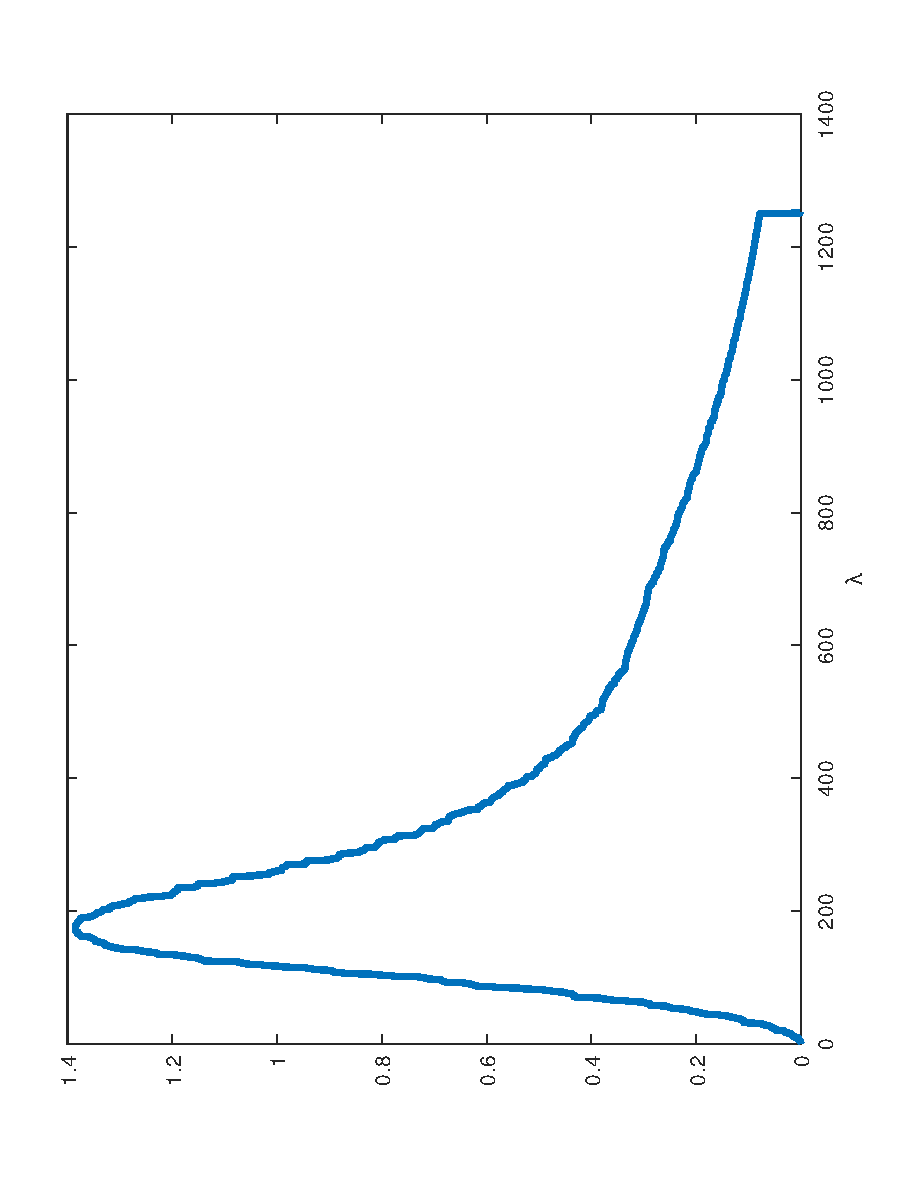
\includegraphics[
        angle=-90,
        origin=c,
        width=\textwidth]{papers/sgwt/images/wavelets/gt3.pdf}
        \vspace{-45pt}
        \caption{Die Kernelfunktion $g(t_3\lambda)$ eines Kugelgraphen mit 1252 
            Knoten und $t_3 = 0.89443$.}
        \label{fig:sgwt:wavelets:sphere:gt3}
    \end{minipage}
    ~
    \begin{minipage}[b]{0.49\textwidth}
        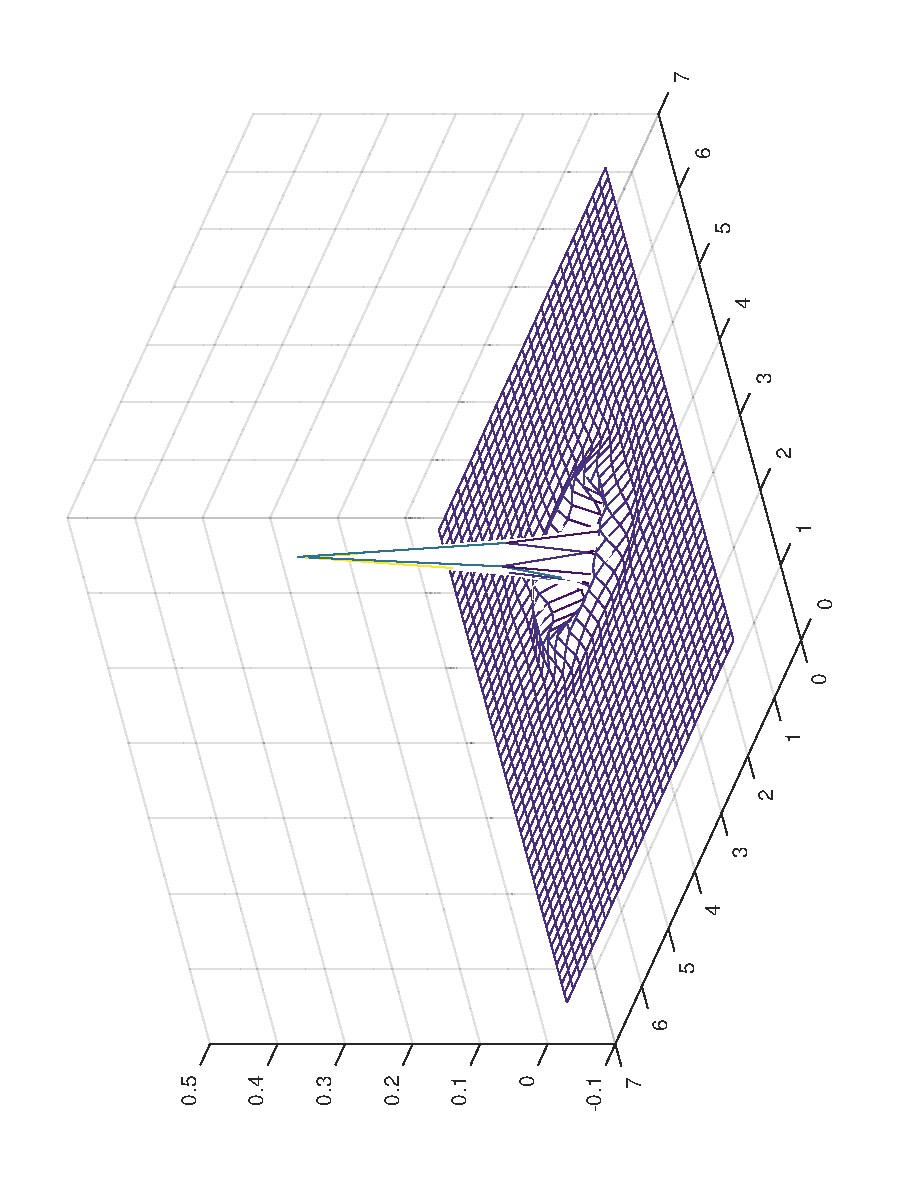
\includegraphics[
        angle=-90,
        origin=c,
        width=\textwidth]{papers/sgwt/images/wavelets/psi_t3_50_25_630_flat.pdf}
        \vspace{-45pt}
        \caption{$\psi_3(v_{630})$-Wavelet eines Kugelgraphen mit 1252 Knoten.}
        \label{fig:sgwt:wavelets:sphere:psi3:flat}
    \end{minipage}
    ~
    \begin{minipage}[b]{\textwidth}
        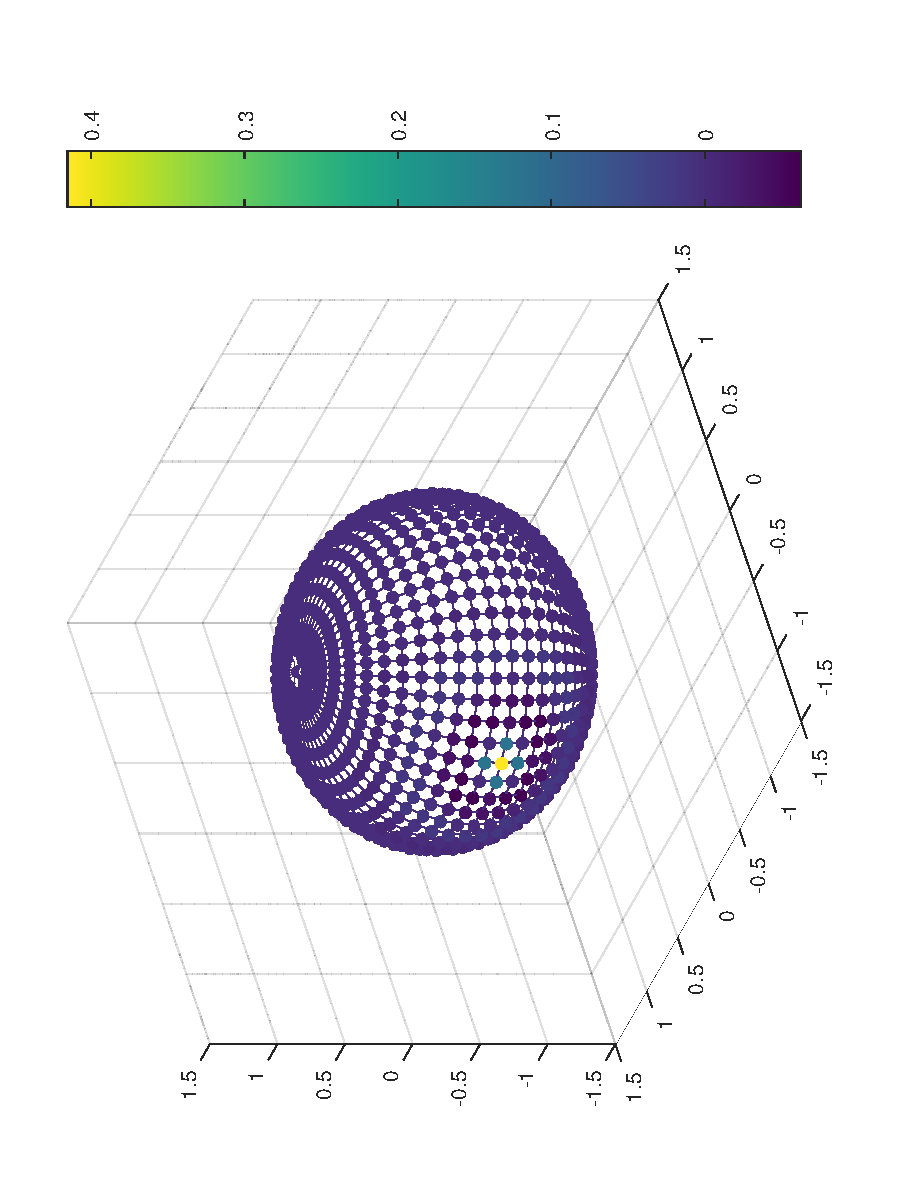
\includegraphics[
        angle=-90,
        origin=c,
        width=\textwidth]{papers/sgwt/images/wavelets/psi_t3_50_25_630.pdf}
        \vspace{-45pt}
        \caption{$\psi_3(v_{630})$-Wavelet eines Kugelgraphen mit 1252 Knoten.}
        \label{fig:sgwt:wavelets:sphere:psi3}
    \end{minipage}
\end{figure}

\begin{figure}
    \begin{minipage}[b]{0.49\textwidth}
        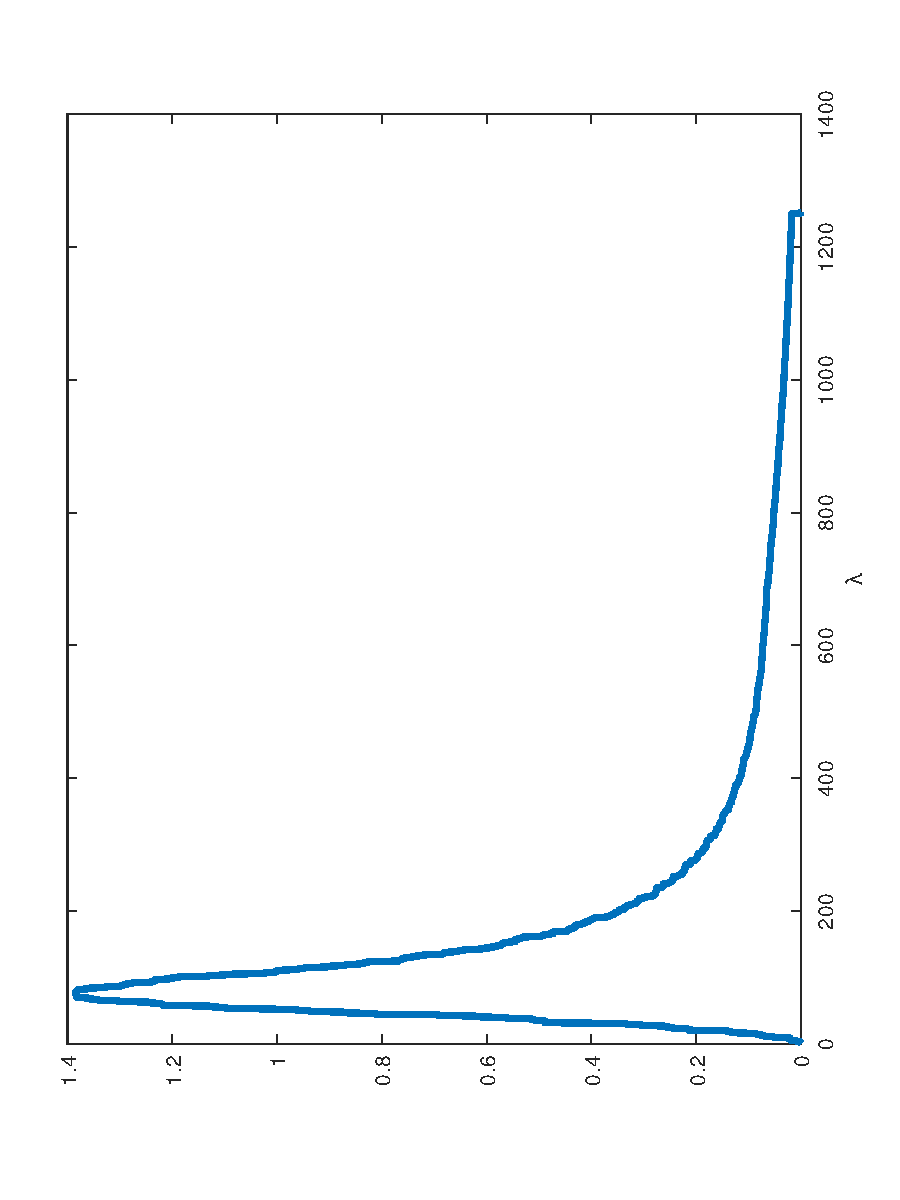
\includegraphics[
        angle=-90,
        origin=c,
        width=\textwidth]{papers/sgwt/images/wavelets/gt4.pdf}
        \vspace{-45pt}
        \caption{Die Kernelfunktion $g(t_4\lambda)$ eines Kugelgraphen mit 1252 
            Knoten und $t_4 = 1.89148$.}
        \label{fig:sgwt:wavelets:sphere:gt4}
    \end{minipage}
    ~
    \begin{minipage}[b]{0.49\textwidth}
        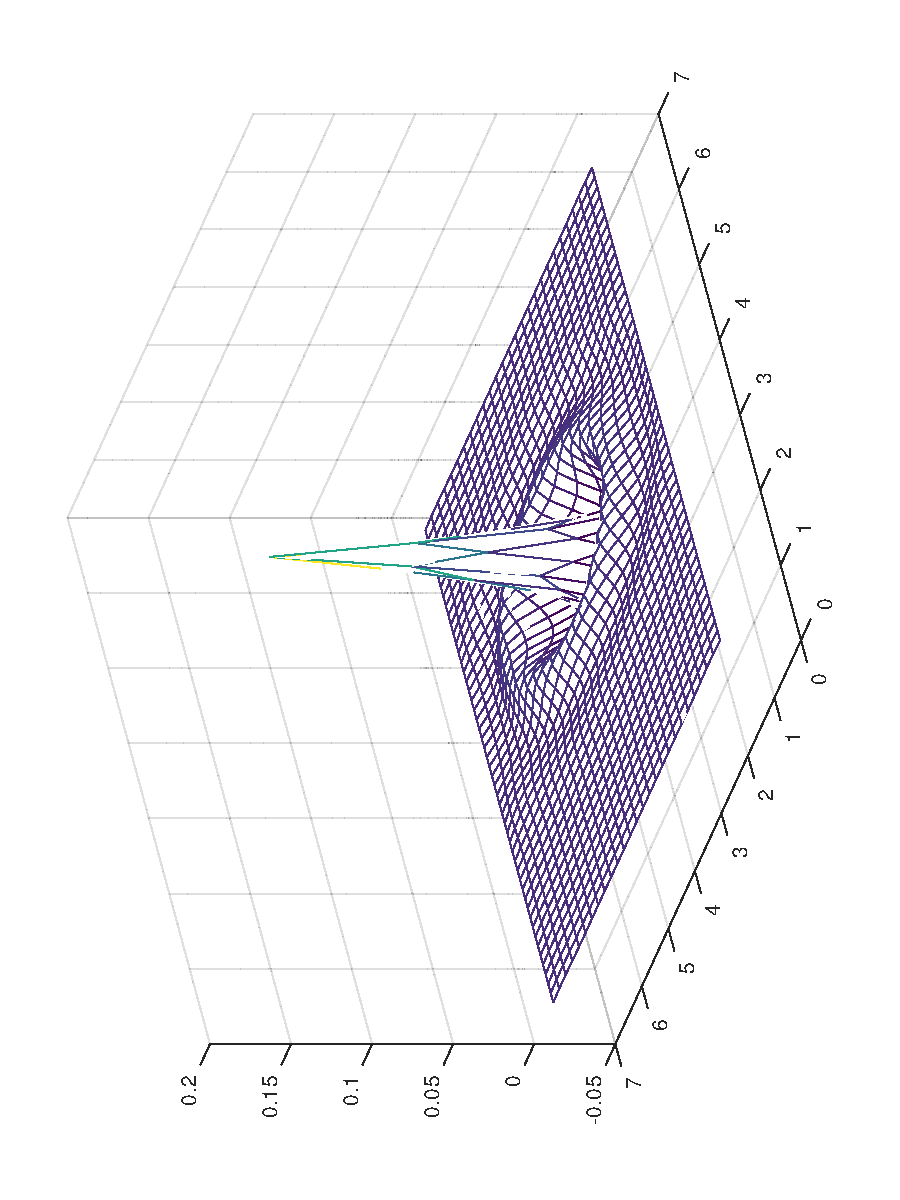
\includegraphics[
        angle=-90,
        origin=c,
        width=\textwidth]{papers/sgwt/images/wavelets/psi_t4_50_25_630_flat.pdf}
        \vspace{-45pt}
        \caption{$\psi_4(v_{630})$-Wavelet eines Kugelgraphen mit 1252 Knoten.}
        \label{fig:sgwt:wavelets:sphere:psi4:flat}
    \end{minipage}
    ~
    \begin{minipage}[b]{\textwidth}
        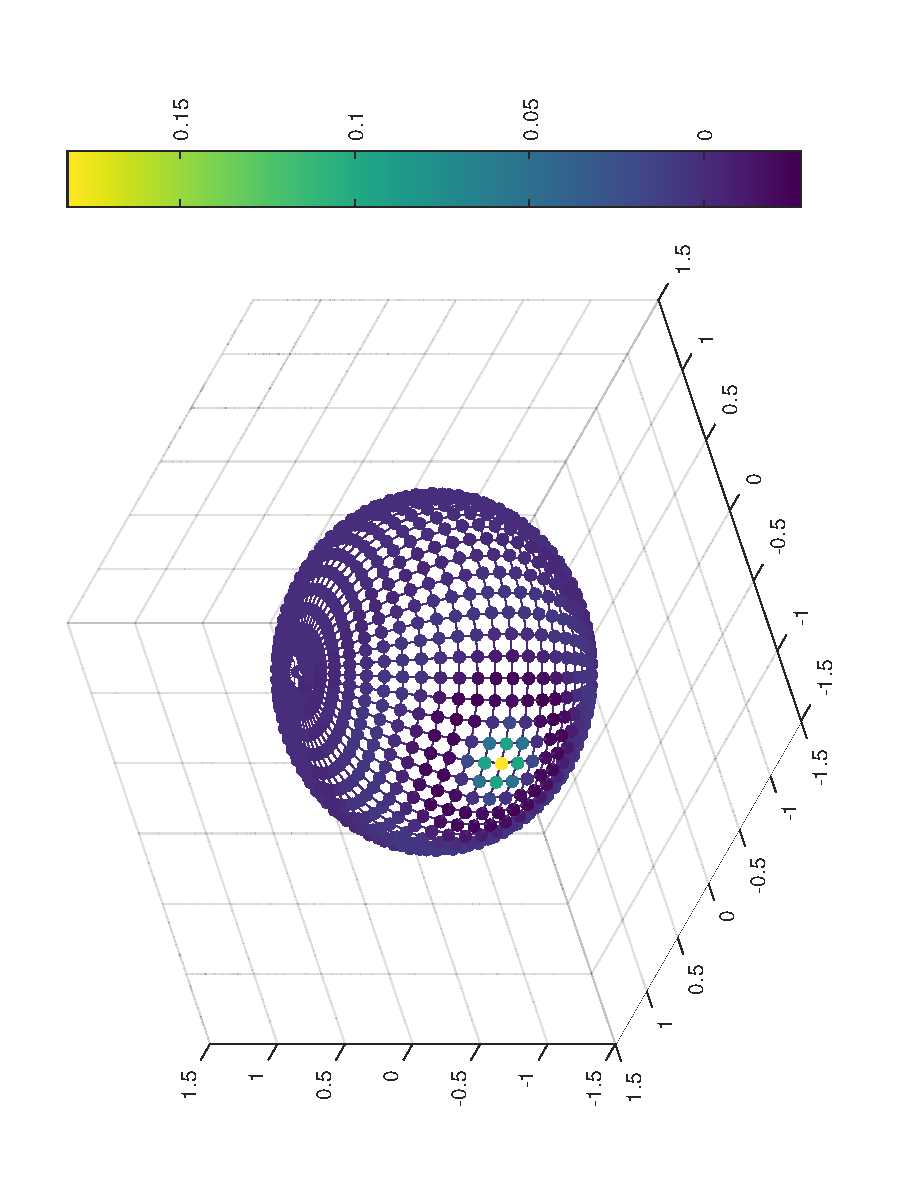
\includegraphics[
        angle=-90,
        origin=c,
        width=\textwidth]{papers/sgwt/images/wavelets/psi_t4_50_25_630.pdf}
        \vspace{-45pt}
        \caption{$\psi_4(v_{630})$-Wavelet eines Kugelgraphen mit 1252 Knoten.}
        \label{fig:sgwt:wavelets:sphere:psi4}
    \end{minipage}
\end{figure}

\begin{figure}
    \begin{minipage}[b]{0.49\textwidth}
        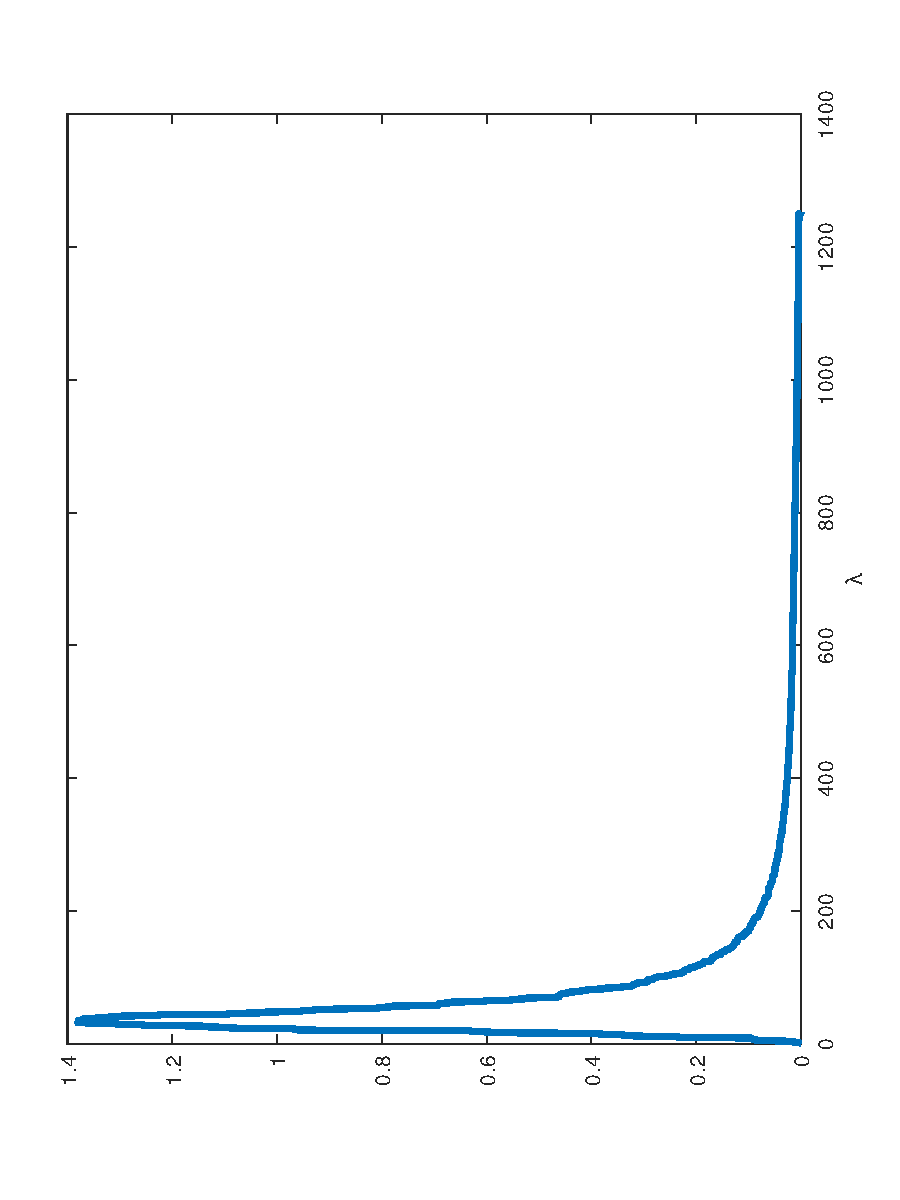
\includegraphics[
        angle=-90,
        origin=c,
        width=\textwidth]{papers/sgwt/images/wavelets/gt5.pdf}
        \vspace{-45pt}
        \caption{Die Kernelfunktion $g(t_5\lambda)$ eines Kugelgraphen mit 1252 
            Knoten und $t_5 = 4$.}
        \label{fig:sgwt:wavelets:sphere:gt5}
    \end{minipage}
    ~
    \begin{minipage}[b]{0.49\textwidth}
        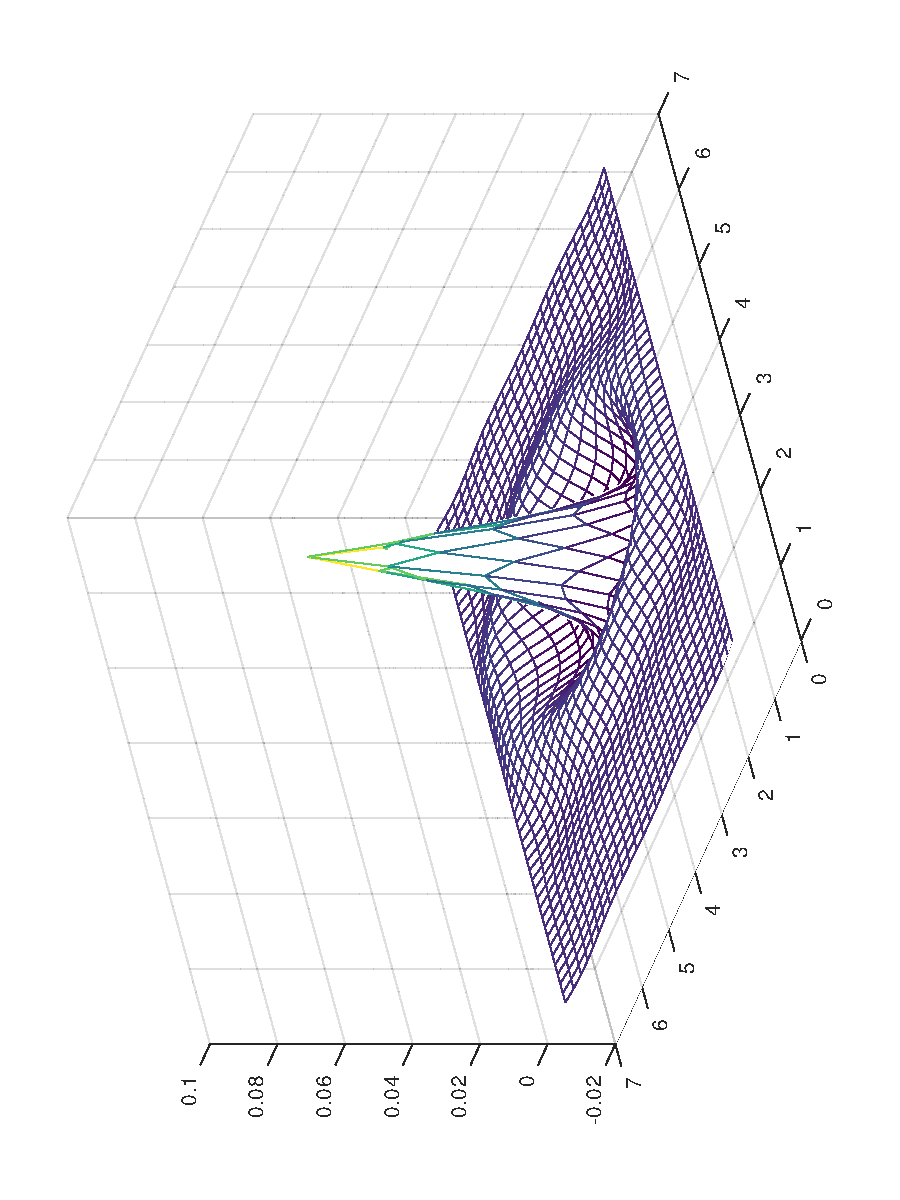
\includegraphics[
        angle=-90,
        origin=c,
        width=\textwidth]{papers/sgwt/images/wavelets/psi_t5_50_25_630_flat.pdf}
        \vspace{-45pt}
        \caption{$\psi_5(v_{630})$-Wavelet eines Kugelgraphen mit 1252 Knoten.}
        \label{fig:sgwt:wavelets:sphere:psi5:flat}
    \end{minipage}
    ~
    \begin{minipage}[b]{\textwidth}
        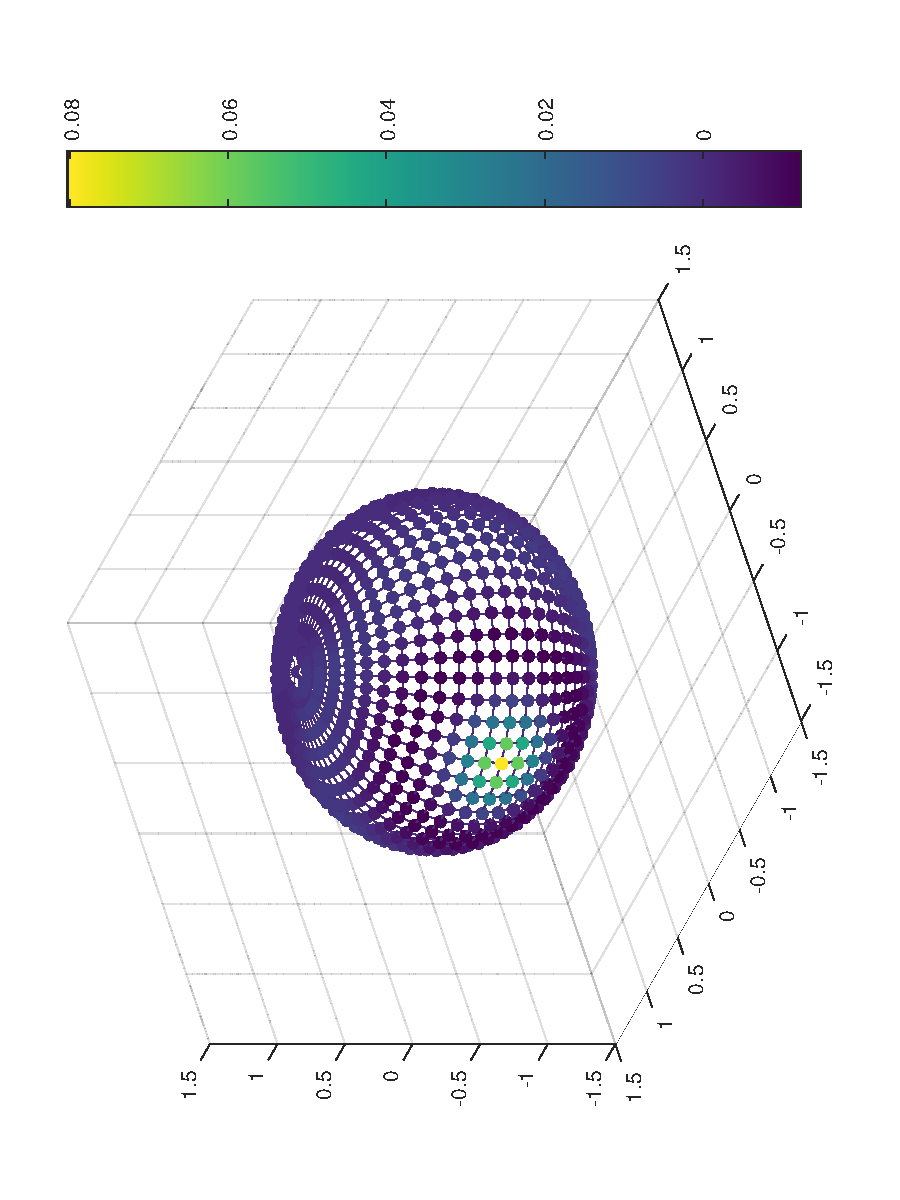
\includegraphics[
        angle=-90,
        origin=c,
        width=\textwidth]{papers/sgwt/images/wavelets/psi_t5_50_25_630.pdf}
        \vspace{-45pt}
        \caption{$\psi_5(v_{630})$-Wavelet eines Kugelgraphen mit 1252 Knoten.}
        \label{fig:sgwt:wavelets:sphere:psi5}
    \end{minipage}
\end{figure}

\begin{figure}
    \begin{minipage}[b]{0.49\textwidth}
        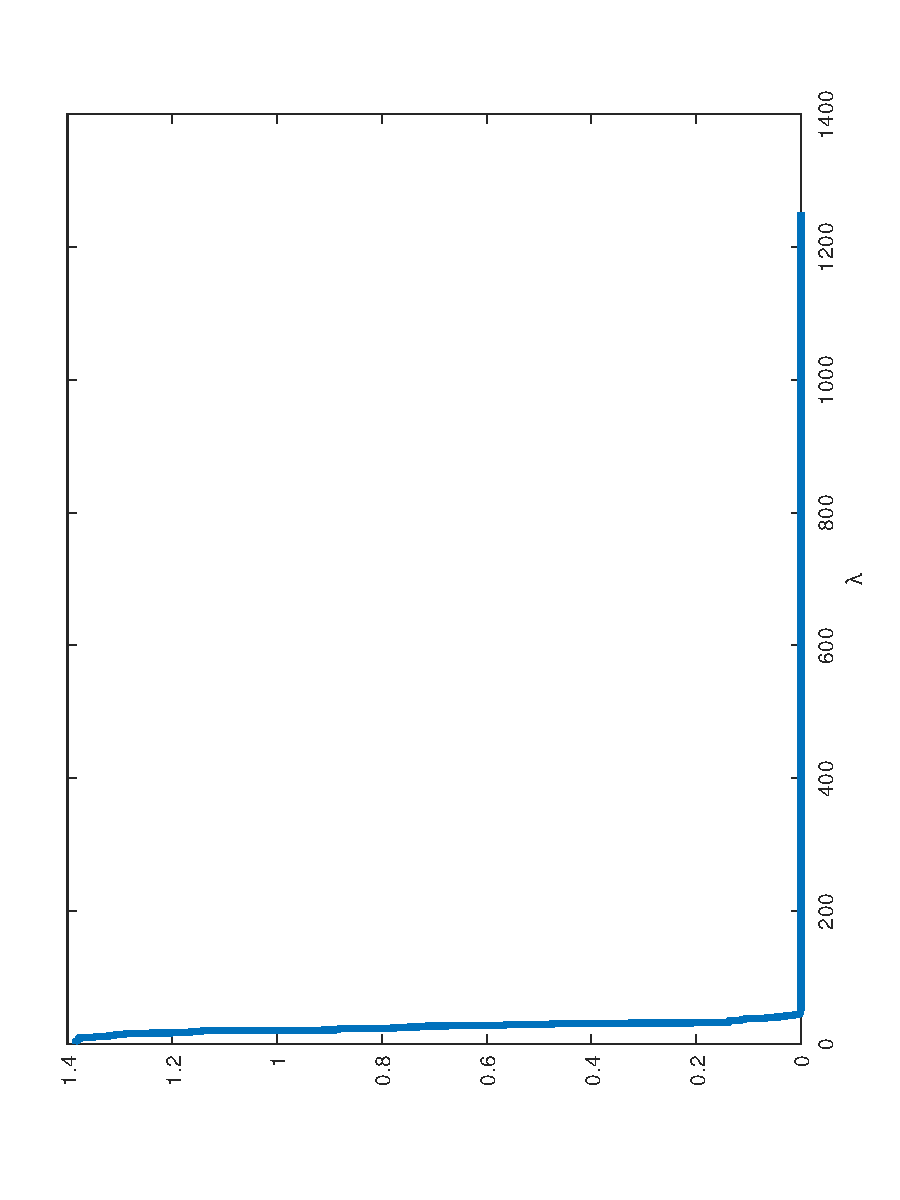
\includegraphics[
        angle=-90,
        origin=c,
        width=\textwidth]{papers/sgwt/images/wavelets/h.pdf}
        \vspace{-45pt}
        \caption{Die Kernelfunktion $h(\lambda)$ eines Kugelgraphen mit 1252 
            Knoten.}
        \label{fig:sgwt:wavelets:sphere:h}
    \end{minipage}
    ~
    \begin{minipage}[b]{0.49\textwidth}
        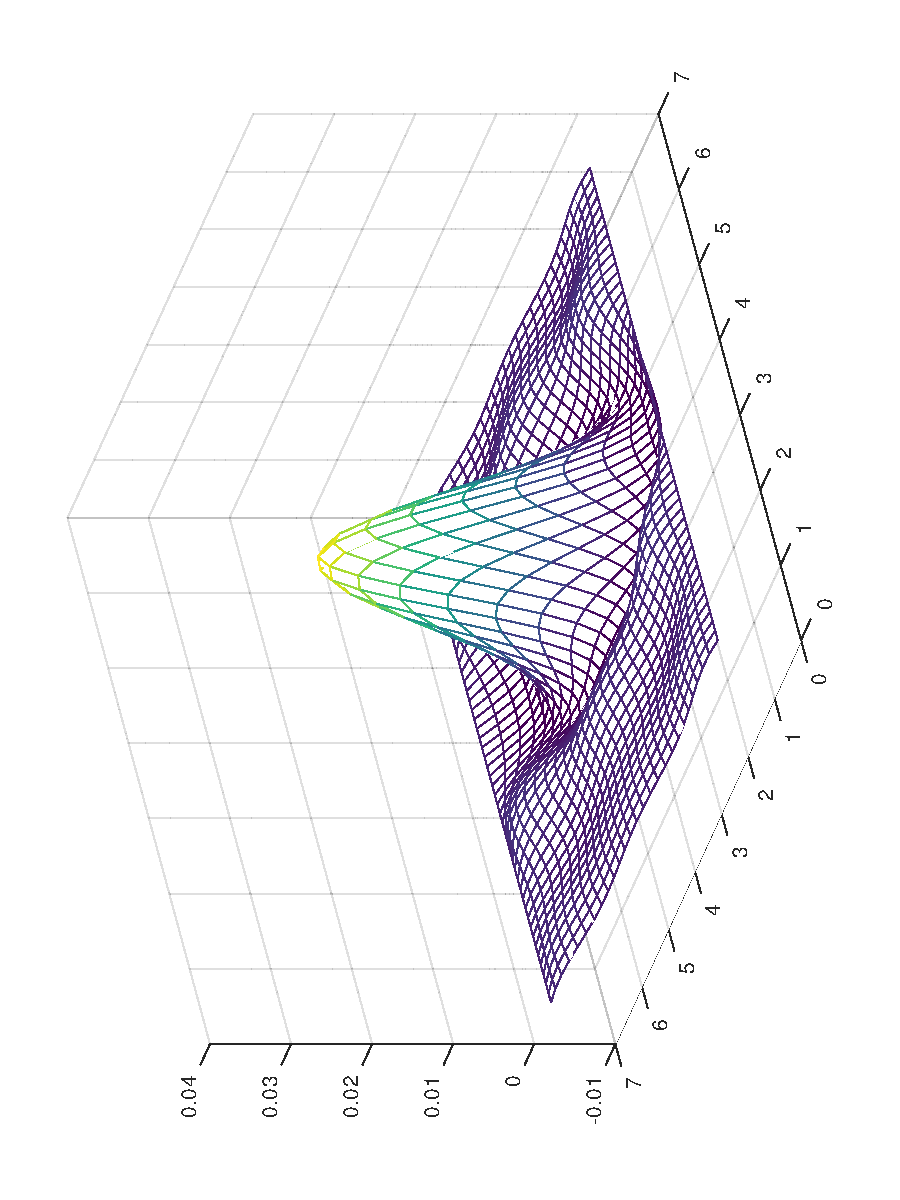
\includegraphics[
        angle=-90,
        origin=c,
        width=\textwidth]{papers/sgwt/images/wavelets/phi_50_25_630_flat.pdf}
        \vspace{-45pt}
        \caption{$\phi(v_{630})$-Wavelet eines Kugelgraphen mit 1252 Knoten.}
        \label{fig:sgwt:wavelets:sphere:phi:flat}
    \end{minipage}
    ~
    \begin{minipage}[b]{\textwidth}
        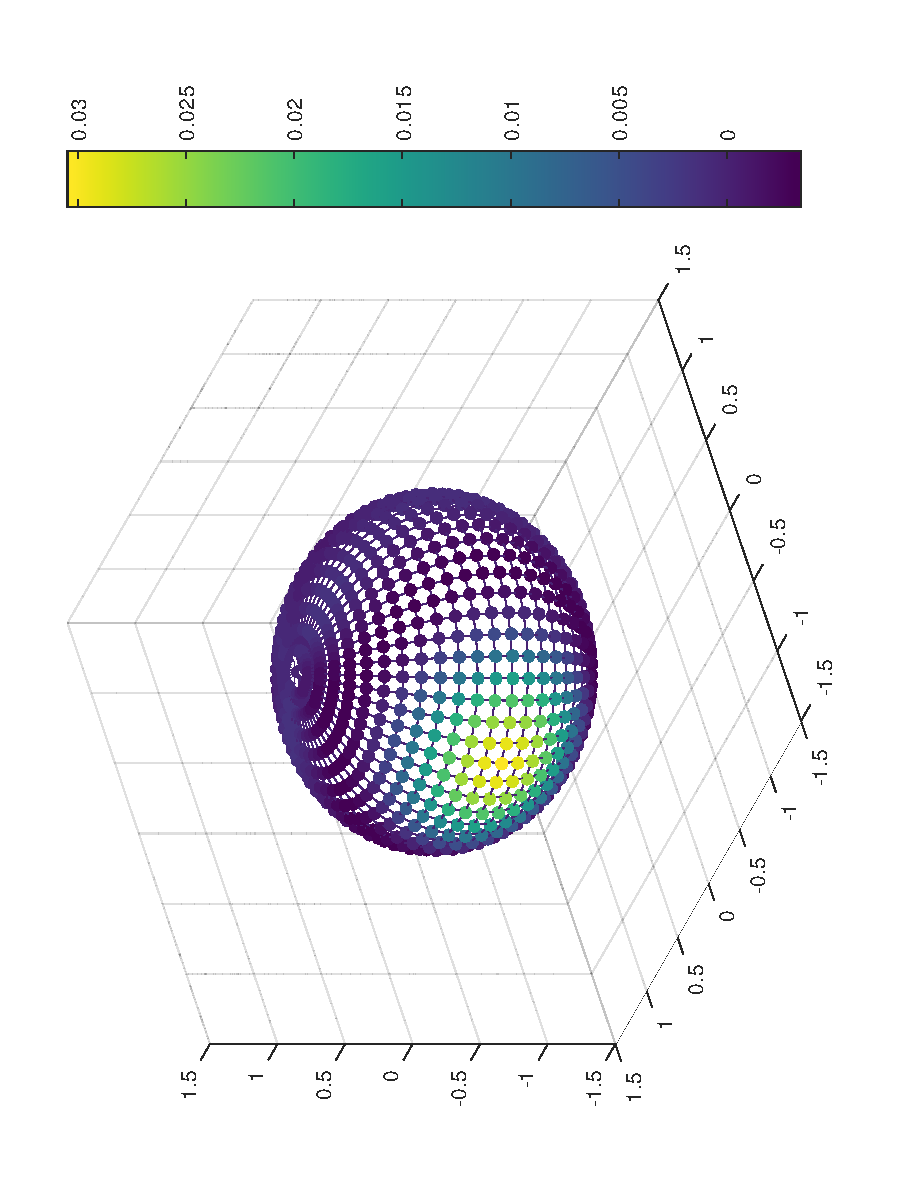
\includegraphics[
        angle=-90,
        origin=c,
        width=\textwidth]{papers/sgwt/images/wavelets/phi_50_25_630.pdf}
        \vspace{-45pt}
        \caption{$\phi(v_{630})$-Wavelet eines Kugelgraphen mit 1252 Knoten.}
        \label{fig:sgwt:wavelets:sphere:phi}
    \end{minipage}
\end{figure}

\subsubsection{Kernelfunktionen}

Um dieses Problem zu l\"osen nehmen wir eine Kernelfunktion $g(\lambda)$, 
welche die Eigenschaften $g(0) = 0$ und $\lim_{\lambda\to\infty} g(x) = 0$ 
erf\"ullt. Mit Hilfe dieses Bandpasses k\"onnen wir die Eigenwerte bewusst 
delokalisieren. Wenn wir nun zus\"atzlich die Eigenwerte mit einem 
Skalierungsfaktor $t$ multiplizieren, erhalten wir auch eine 
M\"oglichkeit, das Spektrum zu verschieben. Obwohl $t$ ein kontinuierlicher 
Faktor ist, werden wir uns in der Praxis auf $J$ Faktoren, also eine endliche 
Anzahl $\{t_j\}^J_{j=1}$, beschr\"anken m\"ussen.

Wir haben jetzt nur noch das Problem, dass $\lambda_0 = 0$ gilt. Wir verlieren 
also den konstanten Anteil der zu analysierenden und synthetisierenden 
Funktion. Um das zu umgehen nehmen brauchen wir eine zus\"atzliche 
Kernelfunktion $h(\lambda)$ mit den Eigenschaften $h(0) > 0$ und 
$\lim_{\lambda\to\infty} = 0$.

Die in~\cref{sec:sgwt:spectralanalysis} vorgestellten Eigenfunktionen 
k\"onnen wir direkt nutzen um eine Graph Fourier Transformation zu definieren. 
Wir ersetzen bei der Fourier Transformation einfach die Exponentialfunktion 
oder Kugelfunktionen durch die Eigenvektoren der Laplace Matrix
\begin{equation*}
\hat{f} = \langle \chi, f \rangle = \sum_{n = 1}^{N} \chi^*(n)f(n).
\end{equation*}
Wenn wir, wie zum Beispiel in \texttt{octave} \"ublich, die Eigenvektoren als 
Spalten einer Matrix
\begin{equation}
\chi = 
\left[
\begin{pmatrix}\\\chi_0\\\\\end{pmatrix}
\begin{pmatrix}\\\chi_1\\\\\end{pmatrix}
\begin{pmatrix}\\\chi_2\\\\\end{pmatrix}
\cdots
\begin{pmatrix}\\\chi_{N-1}\\\\\end{pmatrix}
\right]
\end{equation}
zur Verf\"ugung haben, k\"onnen wir die Transformation 
einfach durch eine Matrix-Vektor Multiplikation ersetzen
\begin{equation*}
\hat{f} = \chi^* f.
\end{equation*}
Die R\"ucktransformation ist dann auch wieder analog der Fouriertheorie
\begin{equation*}
f = \chi \hat{f}.
\end{equation*}

\subsection{Graph Wavelets: Lokalisierung\label{subsec:sgwt:gwt:localizing}}

Mit der Graph Fourier Transformation k\"onnen wir nun Funktionen auf Graphen 
analysieren und dann auch wieder synthetisieren. Mit Hilfe von Wavelets haben 
wir aber bereits gesehen, dass damit auch eine Lokalisierung m\"oglich ist. 
Graphen haben da den Nachteil, dass die Knoten keine inh\"arente Reihenfolge 
haben. Es ist also nicht klar was mit $f(x - h)$ gemeint ist. Wir haben 
allerdings in~\cref{eq:sgwt:lambda:series} eine Reihenfolge f\"ur die 
Eigenwerte der Laplace Matrix eines Graphen definiert. Die Eigenwerte sind 
allerdings komplett lokalisiert, sie kommen also einem Dirac-Stoss an 
einem Knoten gleich.

\subsection{Graph Wavelets: Skalierung\label{subsec:sgwt:gwt:scaling}}

\subsection{Frames}

Mit $h(\lambda)$ und den $J$ skalierten $g(t\lambda)$ haben wir also $J + 1$ 
Kernelfunktionen f\"ur die Analyse und Synthese zur Verf\"ugung. Wir arbeiten 
also mit einem Frame. Die Grenzen sind dabei gegeben als
\begin{align*}
A &= \min_{\lambda \in \left[0, \lambda_{N-1}\right]} f(\lambda) \\
B &= \max_{\lambda \in \left[0, \lambda_{N-1}\right]} f(\lambda) \\
\text{mit } f(\lambda) &= h(\lambda)^2 + \sum_{j = 1}^{J} g(t_j\lambda)^2.
\end{align*}

\subsection{\texorpdfstring{$\psi_j$}{psi} und \texorpdfstring{$\phi$}{phi}}
Damit lassen sich nun unsere Wavelets $\psi_j$ und $\phi$ wie folgt konstruieren
\begin{align}
\psi_j = \chi \diag{g(t_j\lambda)} \chi' 
\label{eq:sgwt:psi}
\\
\phi = \chi \diag{h(\lambda)} \chi'.
\label{eq:sgwt:phi}
\end{align}
Zur Veranschaulichung sehen wir hier die Wavelets eines Kreisgraphen 
in~\cref{fig:sgwt:wavelets:ring0,fig:sgwt:wavelets:ring1,fig:sgwt:wavelets:ring2,fig:sgwt:wavelets:ring3,fig:sgwt:wavelets:ring4,fig:sgwt:wavelets:ring5},
 eines Streckengraphen 
in~\cref{fig:sgwt:wavelets:line0,fig:sgwt:wavelets:line1,fig:sgwt:wavelets:line2,fig:sgwt:wavelets:line3,fig:sgwt:wavelets:line4,fig:sgwt:wavelets:line5}
 und eines Kugelgraphen 
in~\cref{fig:sgwt:wavelets:sphere0,fig:sgwt:wavelets:sphere1,fig:sgwt:wavelets:sphere2,fig:sgwt:wavelets:sphere3,fig:sgwt:wavelets:sphere4,fig:sgwt:wavelets:sphere5}.
Gut zu erkennen ist dabei, dass der Kreisgraph die wohl beste Approximation der 
bisherigen Wavelettheorie ist. Beim Streckengraph fehlt die Periodisierung, die 
wir durch die Verbindungskante des Start- und Endknoten beim Kreisgraphen 
erreicht haben. Auch beim Kugelgraphen wird klar, dass die Pole, aufgrund ihres 
viel gr\"osseren Grades, deutlich st\"arker gewichtet werden und es daher zu 
einer Verzerrung der Wavelets in Richtung der Pole kommt.

\begin{figure}
    \centering
    \begin{minipage}[b]{0.49\textwidth}
        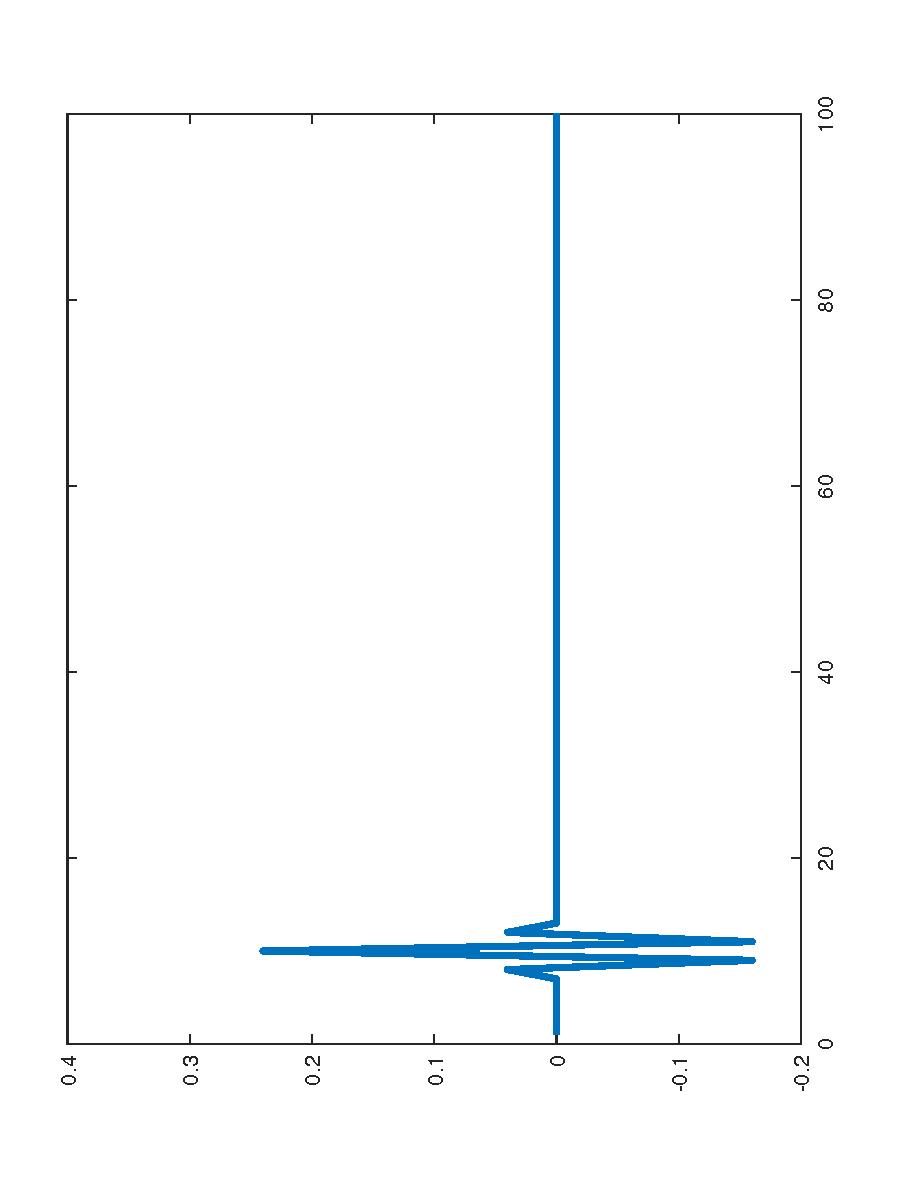
\includegraphics[
        angle=-90,
        origin=c,
        width=\textwidth]{papers/sgwt/images/wavelets-psi-1-10.pdf}
        \vspace{-45pt}
        \caption{$\psi_1(v_{10})$-Wavelets eines Kreisgraphen mit 100 Knoten.}
        \label{fig:sgwt:wavelets:ring0}
    \end{minipage}
    ~
    \begin{minipage}[b]{0.49\textwidth}
        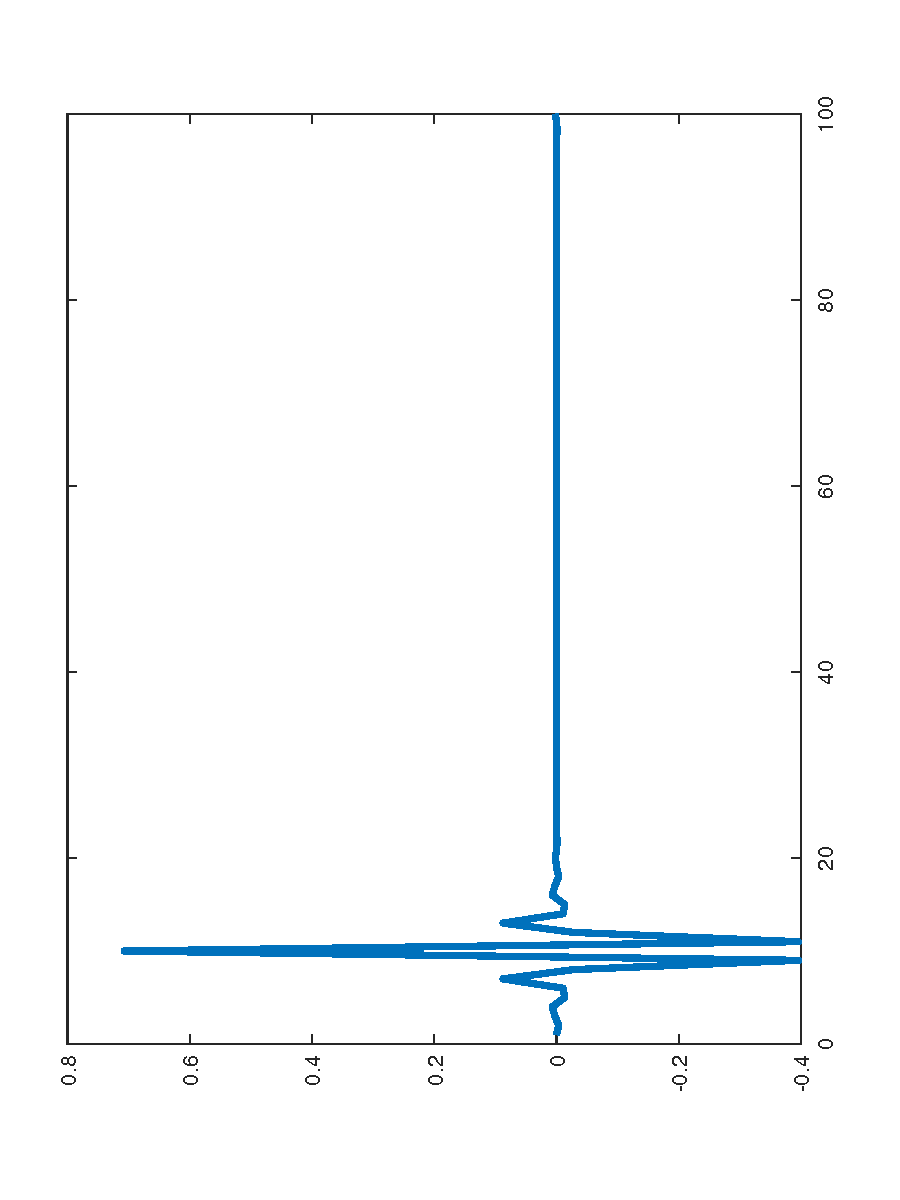
\includegraphics[
        angle=-90,
        origin=c,
        width=\textwidth]{papers/sgwt/images/wavelets-psi-2-10.pdf}
        \vspace{-45pt}
        \caption{$\psi_2(v_{10})$-Wavelets eines Kreisgraphen mit 100 Knoten.}
        \label{fig:sgwt:wavelets:ring1}
    \end{minipage}
    ~
    \begin{minipage}[b]{0.49\textwidth}
        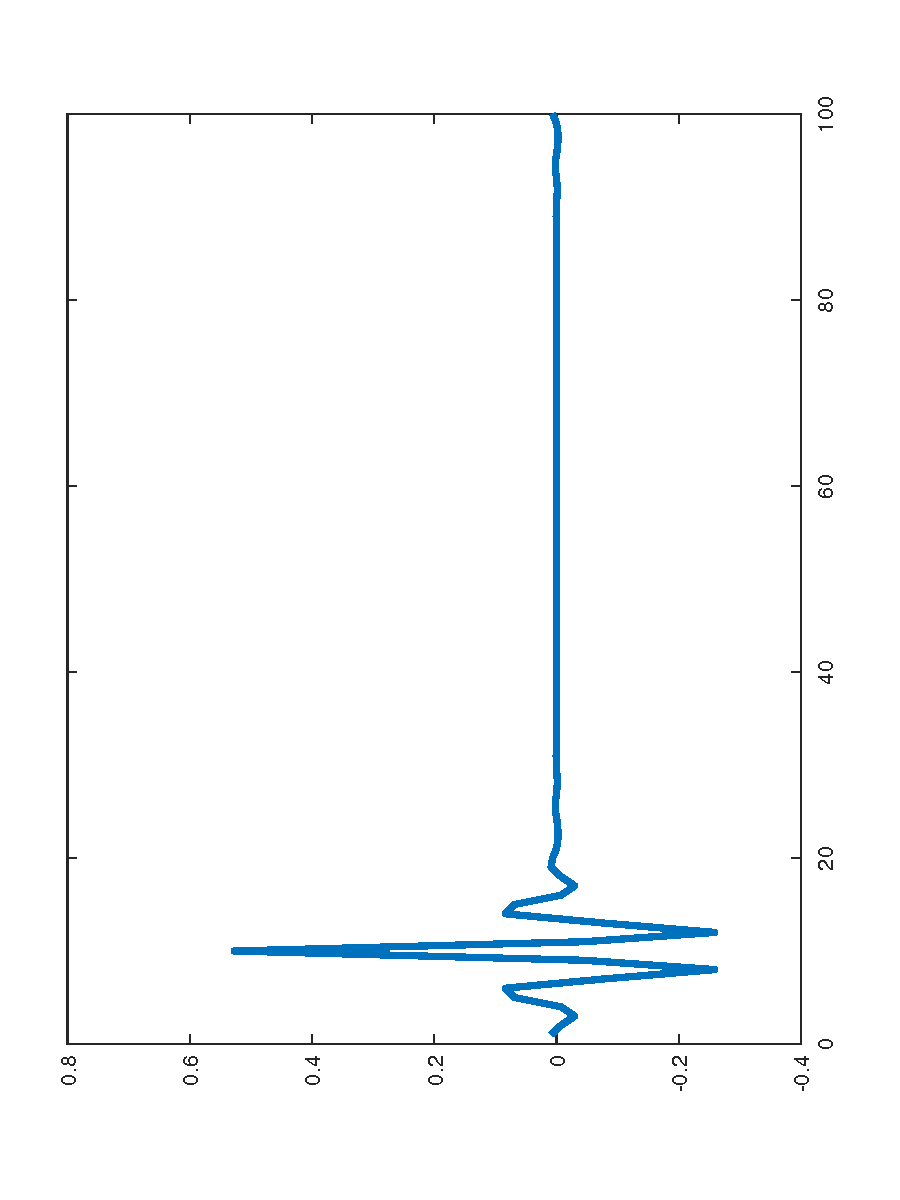
\includegraphics[
        angle=-90,
        origin=c,
        width=\textwidth]{papers/sgwt/images/wavelets-psi-3-10.pdf}
        \vspace{-45pt}
        \caption{$\psi_3(v_{10})$-Wavelets eines Kreisgraphen mit 100 Knoten.}
        \label{fig:sgwt:wavelets:ring2}
    \end{minipage}
    ~
    \begin{minipage}[b]{0.49\textwidth}
        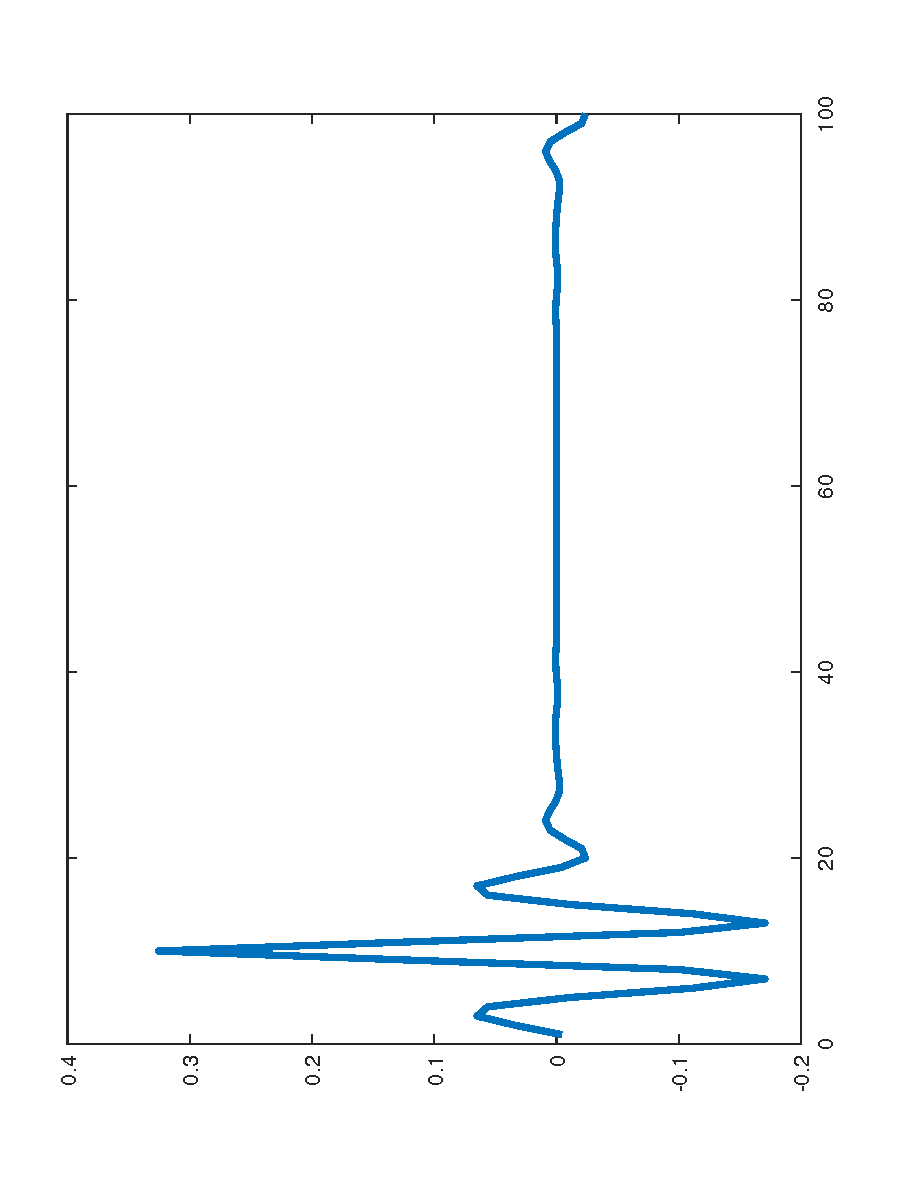
\includegraphics[
        angle=-90,
        origin=c,
        width=\textwidth]{papers/sgwt/images/wavelets-psi-4-10.pdf}
        \vspace{-45pt}
        \caption{$\psi_4(v_{10})$-Wavelets eines Kreisgraphen mit 100 Knoten.}
        \label{fig:sgwt:wavelets:ring3}
    \end{minipage}
    ~
    \begin{minipage}[b]{0.49\textwidth}
        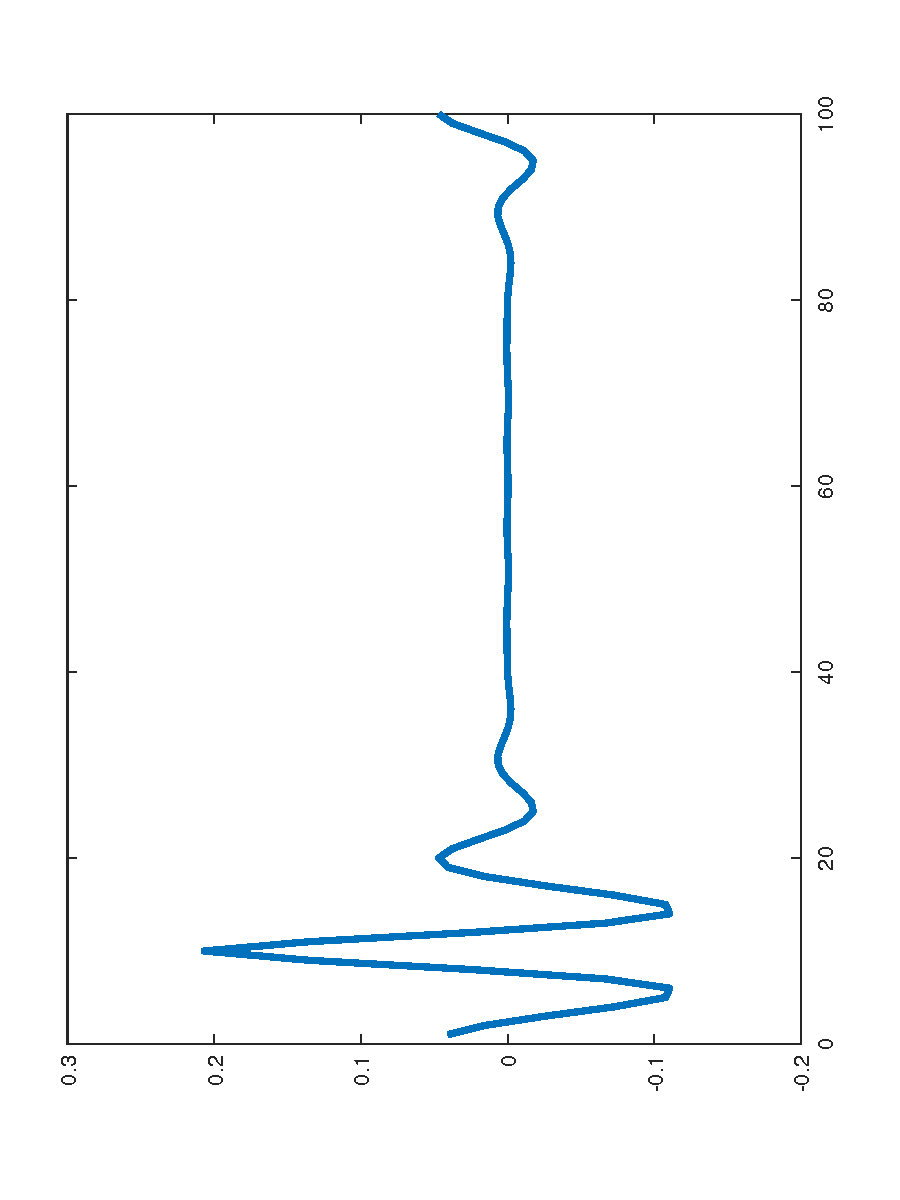
\includegraphics[
        angle=-90,
        origin=c,
        width=\textwidth]{papers/sgwt/images/wavelets-psi-5-10.pdf}
        \vspace{-45pt}
        \caption{$\psi_5(v_{10})$-Wavelets eines Kreisgraphen mit 100 Knoten.}
        \label{fig:sgwt:wavelets:ring4}
    \end{minipage}
    ~
    \begin{minipage}[b]{0.49\textwidth}
        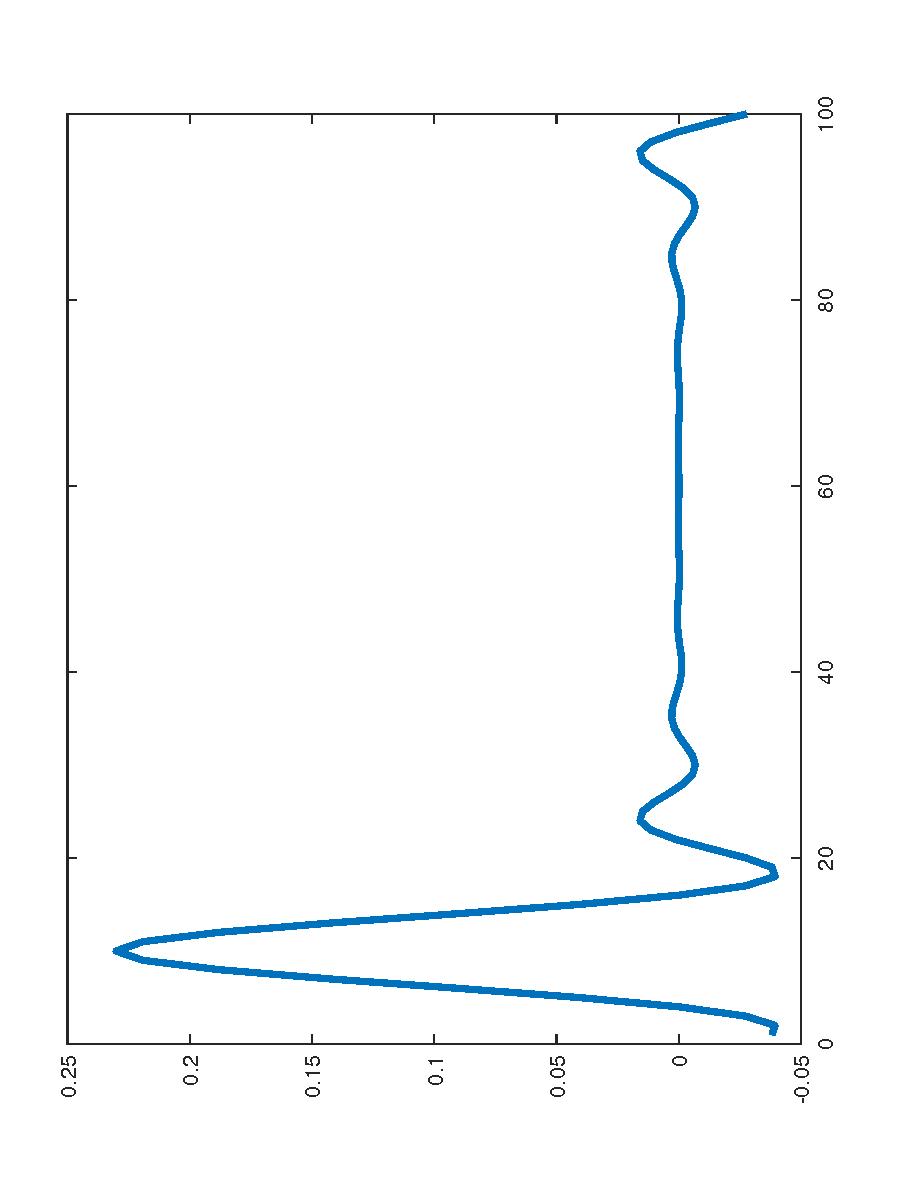
\includegraphics[
        angle=-90,
        origin=c,
        width=\textwidth]{papers/sgwt/images/wavelets-phi-10.pdf}
        \vspace{-45pt}
        \caption{$\phi(v_{10})$-Wavelets eines Kreisgraphen mit 100 Knoten.}
        \label{fig:sgwt:wavelets:ring5}
    \end{minipage}
\end{figure}

\begin{figure}
    \centering
    \begin{minipage}[b]{0.49\textwidth}
        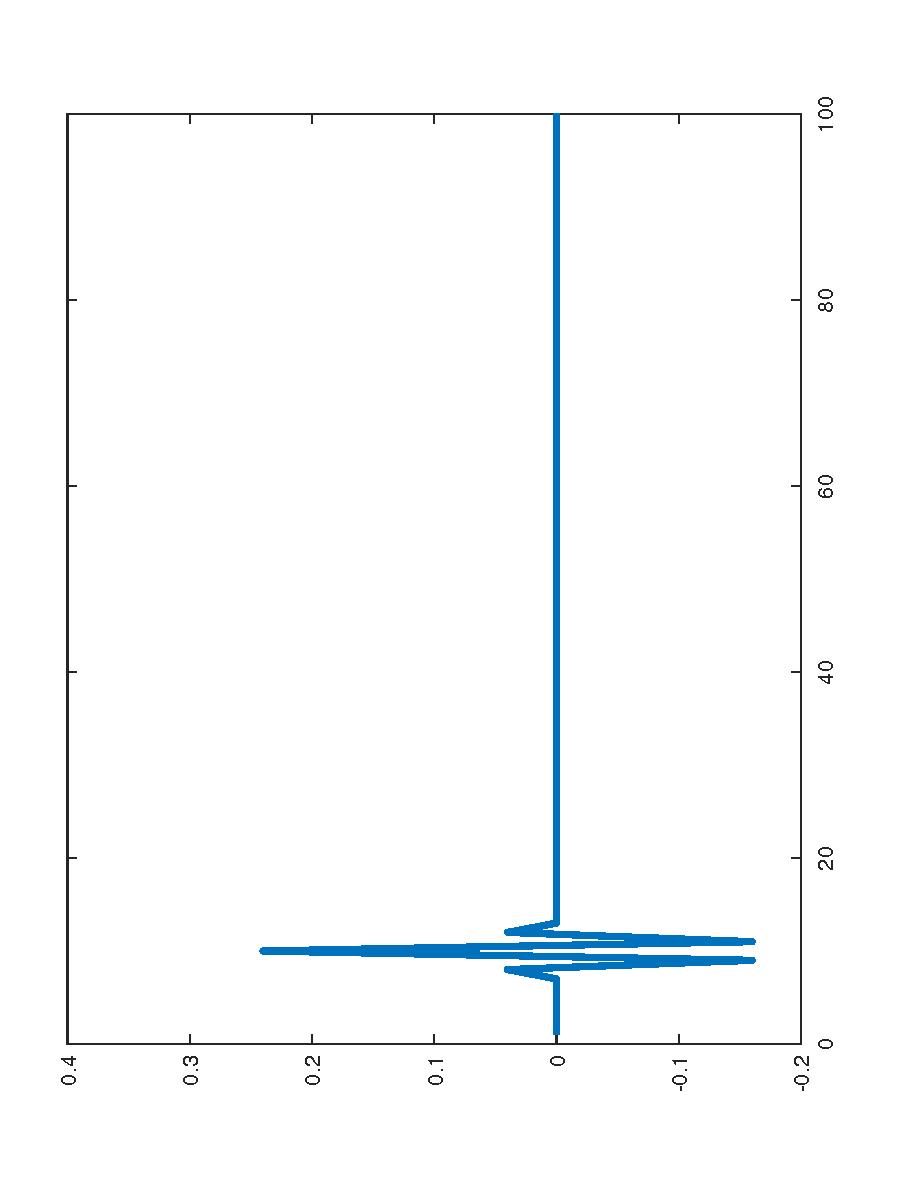
\includegraphics[
        angle=-90,
        origin=c,
        width=\textwidth]{papers/sgwt/images/wavelets-psi-line-1-10.pdf}
        \vspace{-45pt}
        \caption{$\psi_1(v_{10})$-Wavelets eines Streckengraphen mit 100 
        Knoten.}
        \label{fig:sgwt:wavelets:line0}
    \end{minipage}
    ~
    \begin{minipage}[b]{0.49\textwidth}
        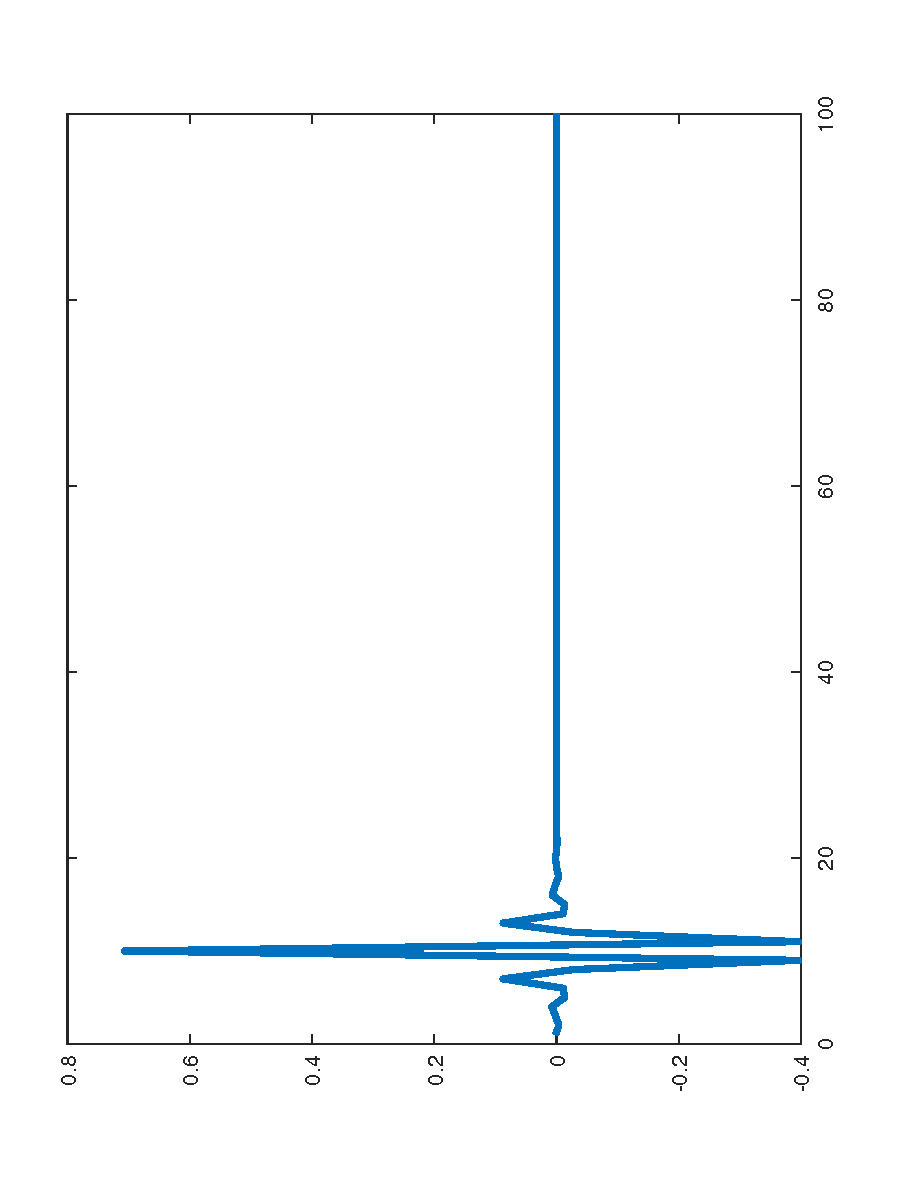
\includegraphics[
        angle=-90,
        origin=c,
        width=\textwidth]{papers/sgwt/images/wavelets-psi-line-2-10.pdf}
        \vspace{-45pt}
        \caption{$\psi_2(v_{10})$-Wavelets eines Streckengraphen mit 100 
        Knoten.}
        \label{fig:sgwt:wavelets:line1}
    \end{minipage}
    ~
    \begin{minipage}[b]{0.49\textwidth}
        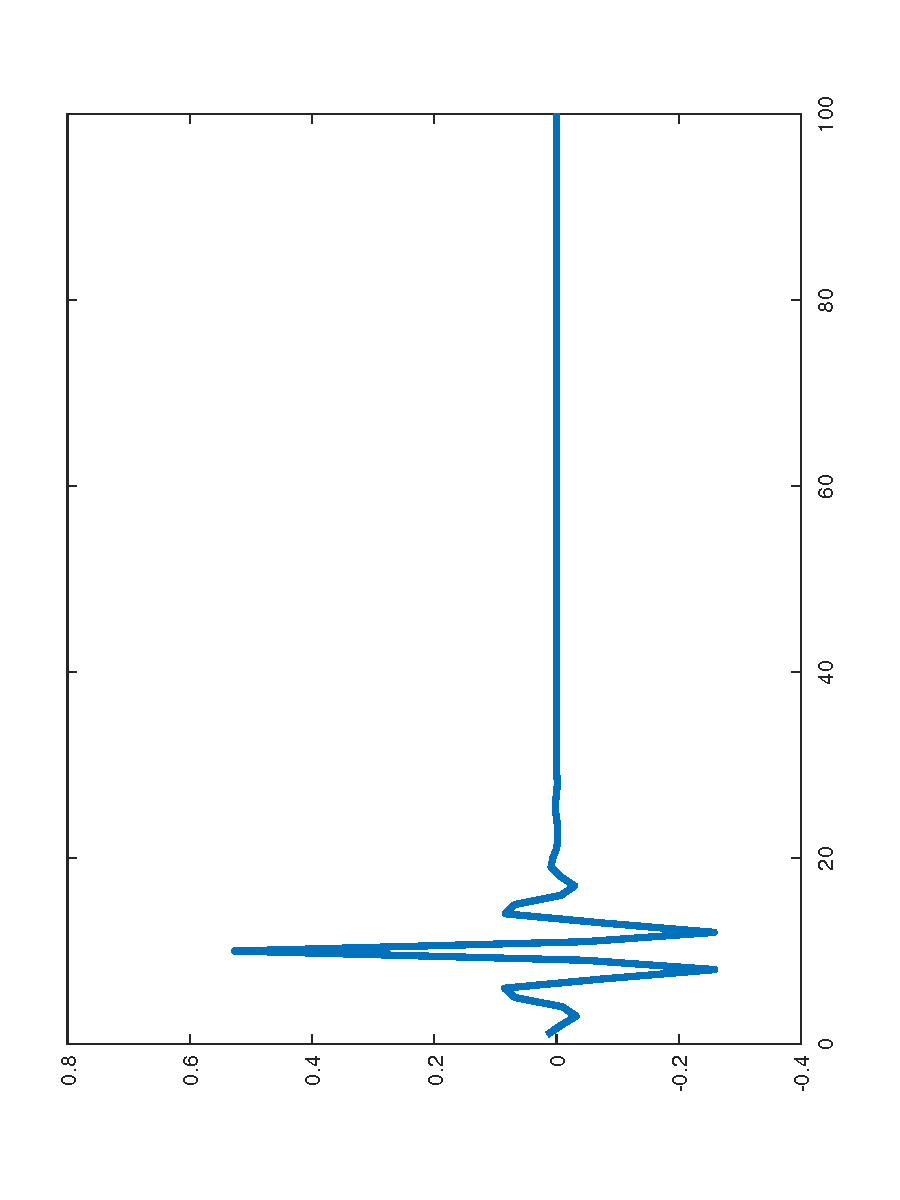
\includegraphics[
        angle=-90,
        origin=c,
        width=\textwidth]{papers/sgwt/images/wavelets-psi-line-3-10.pdf}
        \vspace{-45pt}
        \caption{$\psi_3(v_{10})$-Wavelets eines Streckengraphen mit 100 
        Knoten.}
        \label{fig:sgwt:wavelets:line2}
    \end{minipage}
    ~
    \begin{minipage}[b]{0.49\textwidth}
        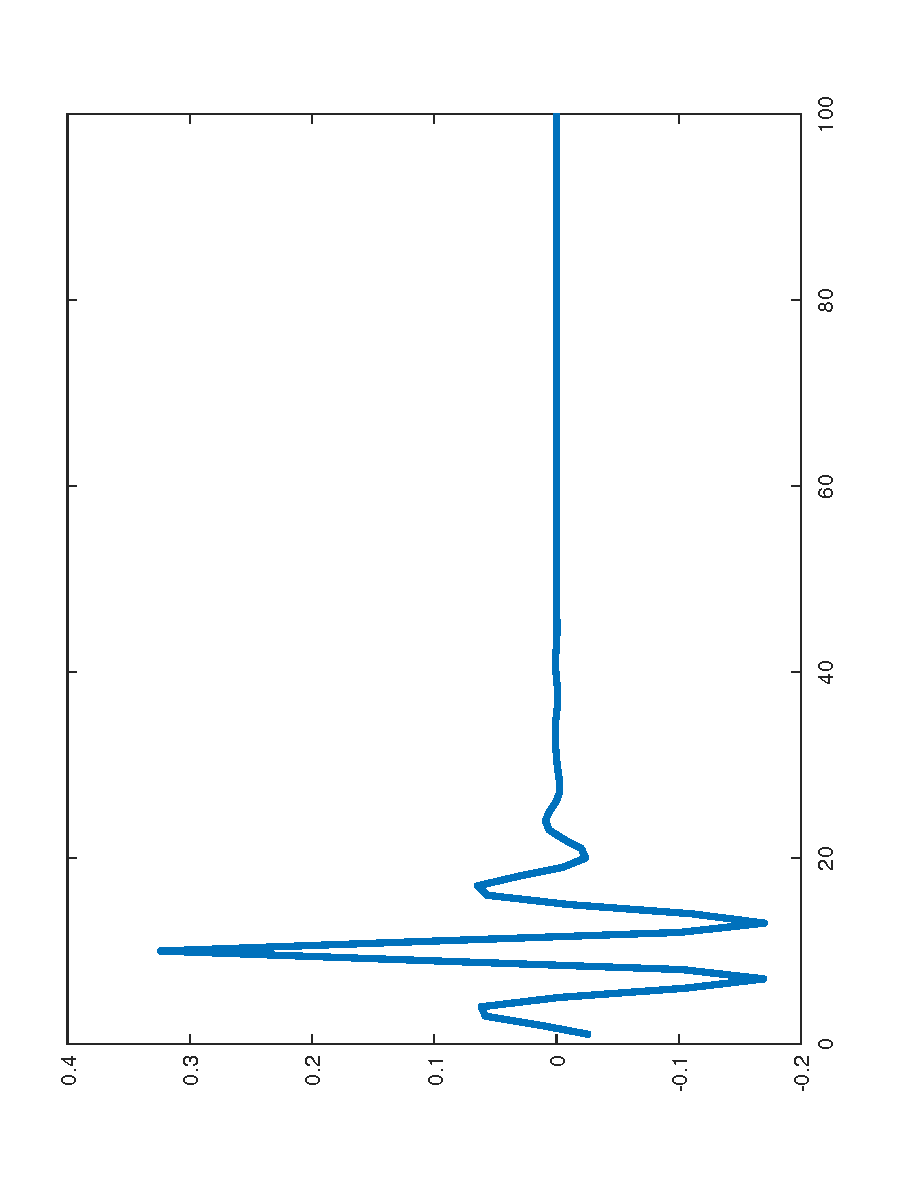
\includegraphics[
        angle=-90,
        origin=c,
        width=\textwidth]{papers/sgwt/images/wavelets-psi-line-4-10.pdf}
        \vspace{-45pt}
        \caption{$\psi_4(v_{10})$-Wavelets eines Streckengraphen mit 100 
        Knoten.}
        \label{fig:sgwt:wavelets:line3}
    \end{minipage}
    ~
    \begin{minipage}[b]{0.49\textwidth}
        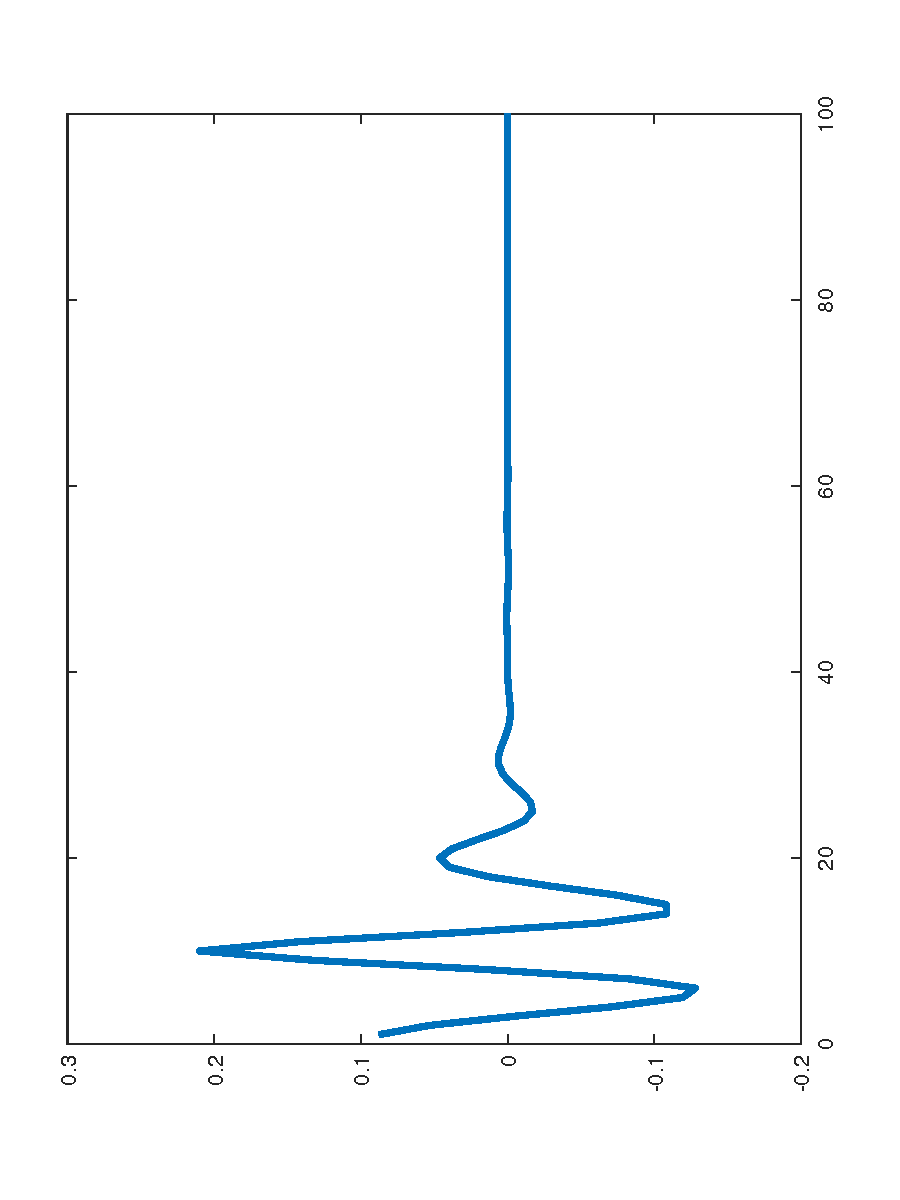
\includegraphics[
        angle=-90,
        origin=c,
        width=\textwidth]{papers/sgwt/images/wavelets-psi-line-5-10.pdf}
        \vspace{-45pt}
        \caption{$\psi_5(v_{10})$-Wavelets eines Streckengraphen mit 100 
        Knoten.}
        \label{fig:sgwt:wavelets:line4}
    \end{minipage}
    ~
    \begin{minipage}[b]{0.49\textwidth}
        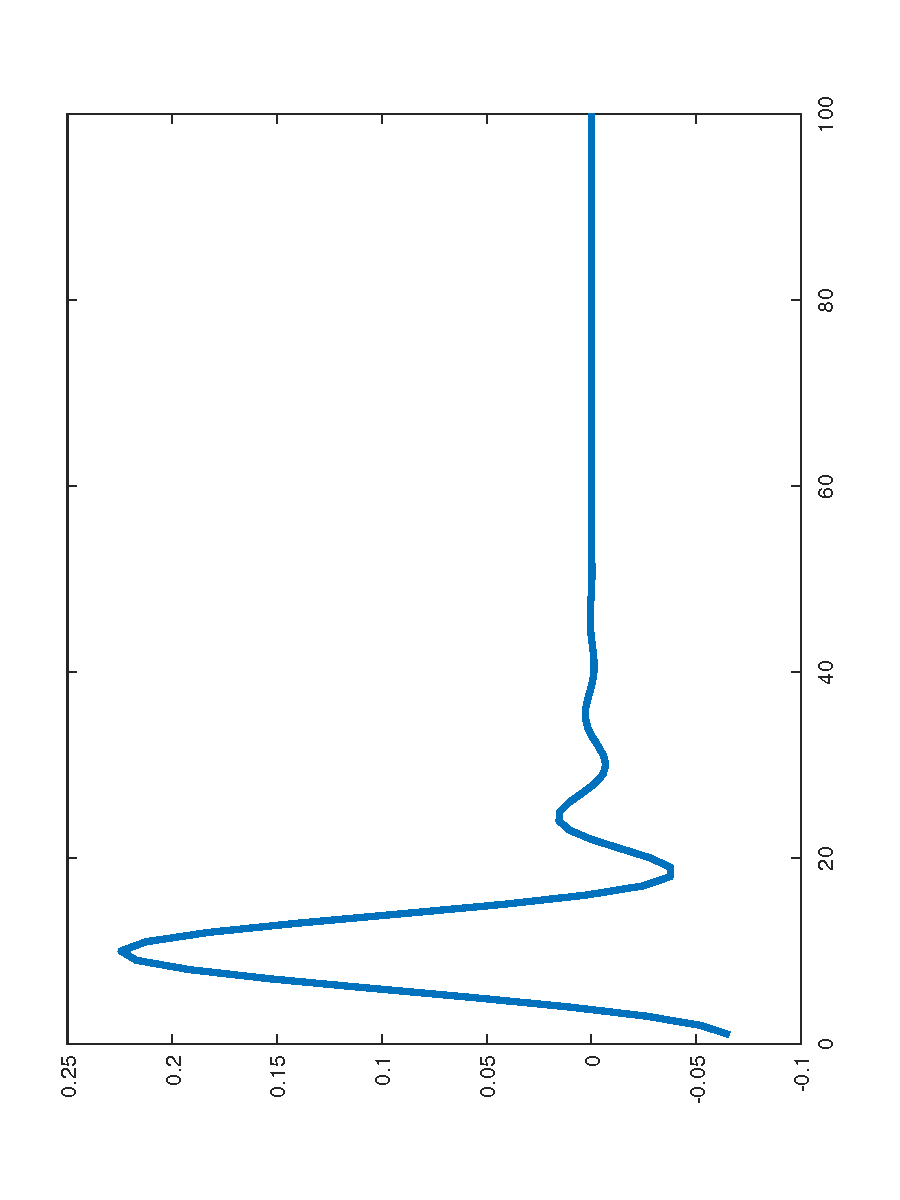
\includegraphics[
        angle=-90,
        origin=c,
        width=\textwidth]{papers/sgwt/images/wavelets-phi-line-10.pdf}
        \vspace{-45pt}
        \caption{$\phi(v_{10})$-Wavelets eines Streckengraphen mit 100 Knoten.}
        \label{fig:sgwt:wavelets:line5}
    \end{minipage}
\end{figure}

Die Wavelets k\"onnen wir dann wieder ein die $N(J+1)\text{x}N$-Matrix $T$ 
packen um dann die Wavelet Koeffizienten wie folgt zu berechnen
\begin{equation}
\hat{f} = T f.
\label{eq:sgwt:hatf}
\end{equation}

\subsection{SGWT Analyse und Synthese}

Um nun eine Funktion $f(v)$ auf einem Graphen $G$ zu analysieren gehen wir 
also wie folgt vor:
\begin{itemize}
    \item[1.] Generierung der \laplaceL{} Matrix aus dem Graphen $G$.
    \item[2.] Berechnung der Eigenwerte $\lambda$ und Eigenvektoren $\chi$.
    \item[3.] Berechnung der $\psi_j$ und $\phi$ Wavelets 
    mit~\cref{eq:sgwt:psi,eq:sgwt:phi}.
    \item[4.] Berechnung der Wavelet Koeffizienten $\hat{f}$ 
    mit~\cref{eq:sgwt:hatf}.
\end{itemize}

F\"ur die Synthese nehmen wir als Eingabe die bei der Analyse berechnet und 
danach m\"oglicherweise bearbeiteten $\hat{f}$. Zus\"atzlich brauchen wir die 
$T$ Matrix, mit deren Inversen wir wieder die Funktion
\begin{equation}
f = T^{-1} \hat{f}
\end{equation}
synthetisieren. Da diese Matrix aber nicht mehr quadratisch ist, kann sie nicht 
mehr so einfach invertiert werden. Wir nehmen uns daher das Pseudoinverse $L = 
(T^*T)^{-1}T^*$ zur Hilfe und erhalten
\begin{equation}
f = L \hat{f} = (T^*T)^{-1}T^* \hat{f}.
\end{equation}

\section{Effiziente Berechnung der CWT}
\rhead{Berechnung der CWT}
Als erstes möchten wir herausfinden, wie sich die CWT effizient berechnen lässt.
Als zweites werden wir zwei Beispielsignale definieren und die CWT mittels Haar-Wavelet betrachten.
Abschliessend rechnen wir die CWT noch mit dem Gabor-Wavelet und vergleichen die beiden Bilder.

\subsection{CWT als Faltung}
Betrachten wir zuerst die folgende Gleichung
\begin{equation}
\Wave f (a,b)
=
\langle f,\psi_{a,b}\rangle
=
\frac{1}{\sqrt{|a|}}\int_{-\infty}^\infty f(t)\,
	\overline{\psi}\biggl(\frac{t-b}{a}\biggr)\,dt,\label{complex:CWT}
\end{equation}
durch welche in Definition~\ref{cwt:definition} die kontinuierliche Wavelet-Transformation eingeführt wurde.
Dieses Integral entspricht der Faltung zwischen $f(t)$ und 
\begin{equation} 
    g(t) 
    = \frac{1}{\sqrt{|a|}} \overline\psi\biggl(\frac{-t}{a}\biggr).
\end{equation}
Der Standard-Trick zur effizienten Berechnung einer Faltung ist die Multiplikation im Frequenzbereich.
\begin{equation} 
\mathcal{W}f (a,b) = (f*g)(t) = \mathcal{F}^{-1}\biggl\lbrace\hat f(\omega) \hat g (\omega) \biggr\rbrace.
\end{equation}
Dafür benötigen wir die Fouriertransformierte $\hat g (\omega)$:
\begin{align*}
	\hat g (\omega) = 
    \Four\,\biggl\lbrace \frac{1}{\sqrt{|a|}} \overline\psi \biggl(\frac{-t}{a}\biggr) \biggr\rbrace 
	&= \frac{1}{\sqrt{|a|}} \int_{-\infty}^{\infty}\overline\psi\biggl(\frac{-t}{a}\biggr) \, e^{-i\omega t}\,dt\\
	&= \frac{1}{\sqrt{|a|}} \overline{\int_{-\infty}^{\infty}\psi \biggl(\frac{-t}{a}\biggr) \, e^{i\omega t}\,dt}  
    & \biggl(\text{Substitution } t' = \frac{-t}{a}\biggr)\\
	&= \frac{1}{\sqrt{|a|}} \overline{\int_{-\infty}^{\infty}\psi(t') \, e^{-ia\omega t'} |a|\,dt'}\\
	&= \sqrt{|a|} \, \overline{\hat{\psi}}(a\omega).
\end{align*}
Gleichung~\eqref{complex:CWT} lässt sich somit schreiben als
\begin{equation}
\Wave f(a,b)
= \mathcal{F}^{-1}\bigl\lbrace\hat{f}(\omega) \sqrt{|a|}\, \overline{\hat{\psi}}(a\omega)\bigr\rbrace. \label{complex:fcwt}
\end{equation}

Mittels Fourier-Transformation lässt sich die Wavelet-Transformation folglich besonders elegant berechnen.
Kontinuierliche Funktionen sind für numerische Systeme jedoch ungeeignet.
Die CWT muss in $a$ und $b$ diskretisiert werden.
Die Diskretisierung von $b$ entspricht vorteilhaft gerade derjenigen des Signals selbst.
Dann lässt sich die Fourier-Transformation mittels FFT effizient berechnen und Gleichung~\eqref{complex:fcwt} wird zu
\begin{equation}
	\mathcal{W}f(a,b) = \text{IFFT}\bigl(\text{FFT}(f) \, \overline{\hat{\psi}}(a\omega)\bigr). \label{complex:ffcwt}
\end{equation}

Der Faktor $\sqrt{|a|}$ wurde hierbei weggelassen.
Hierdurch werden die hohen Frequenzen stärker gewichtet und $|\!\Wave f(a,b)|$ ist gerade proportional zur Amplitude der analysierten Signalkomponente.
Zudem erzielen wir im Diskreten nicht exakt die Faltung, sondern die zirkuläre Version davon. 
Mehr dazu im Abschnitt~\ref{complex:circ-conv-padding}.

Gleichung~\eqref{complex:ffcwt} muss für jedes $a$ einzeln gelöst werden.
Sie wird besonders interessant, wenn das Wavelet im Frequenzbereich eine geschlossene, analytische Form besitzt.
Dann benötigt man nur eine FFT für das Signal, so wie für jedes $a$ eine inverse FFT und eine punktweise Multiplikation zwischen Signal und Wavelet.

%\clearpage
\subsection{Das Haar-Wavelet}
\rhead{Haar-Wavelet}
\begin{figure}
	\centering
	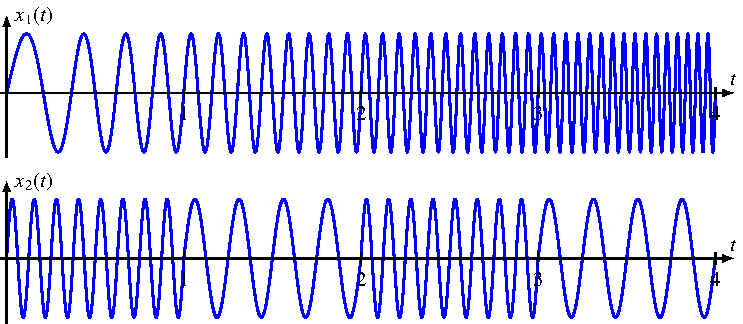
\includegraphics{papers/complex/images/signals.pdf}
	\caption{Die beiden Beispielsignale $x_1(t)$ und $x_2(t)$}
\end{figure}
Rechnen wir das erste Beispiel.
Hierfür benötigen wir zwei Dinge: Signal und Wavelet.
Als Signale nehmen wir zwei Sinus-Schwingungen, eine mit linear ansteigender und eine mit stückweise konstanter Frequenz.
\begin{align}
    x_1(t) &= \sin\left( \int_{0}^{t} 2\pi f_1(\tau)\,d\tau\right) & f_1(t) &= 2 + 6/4 \cdot t \\
    x_2(t) &= \sin\left( \int_{0}^{t} 2\pi f_2(\tau)\,d\tau\right) & f_2(t) &= \left\lbrace \begin{matrix}
    4, & &t& < 1\\
    8, & 1.0 \le &t& < 2.0\\
    4, & 2.0 \le &t& < 3.0\\
    8, & 3.0 \le &t&\\
    \end{matrix}\right.
\end{align}
Das Haar-Wavelet sei in diesem Abschnitt zentriert um $t=0$.
Die daraus resultierende Symmetrie wird sich in der Berechnung der Fourier-Transformation als hilfreich erweisen.

\begin{definition}
	\label{complex:def-haar-wavelet}
	Das Haar-Wavelet besitzt folgende Gestalt:
	\[
	\psi_{\text{Haar}}(t) = \left\lbrace\begin{matrix*}[r]
	1 & -\frac{1}{2} \le t < 0  \\
	-1 & 0 \le t < \frac{1}{2} \\
	0 & \text{sonst}.
	\end{matrix*} \right.\label{complex:def-haar}
	\]
\end{definition}
Die Fourier-Transformierte von $\psi_{\text{Haar}}$ berechnet sich wie folgt:
\begin{align}
	\Four \psi_\text{Haar}  
	&= \frac{1}{\sqrt{2\pi}}\int_{-\infty}^{\infty} \psi_\text{Haar} e^{-i\omega t} \,dt\nonumber\\
	&= \frac{1}{\sqrt{2\pi}}\Biggl( \int_{-1/2}^{0} e^{-i\omega t} \,dt - \int_{0}^{1/2} e^{-i\omega t}\,dt \Biggr) \nonumber\\
	&= \frac{i}{\sqrt{2\pi}\omega}\bigl( \bigl[ e^{-i\omega t}\bigr]_{-1/2}^0  - \bigl[ e^{-i\omega t}\bigr]_{0}^{1/2} \bigr)\nonumber\\
	&= \frac{i}{\sqrt{2\pi}} \frac{1-\cos(\omega/2)}{\omega/2}\label{complex:f-psi-haar}
\end{align}
Das Haar-Wavelet ist also nicht nur im Zeit-, sondern auch im Frequenzbereich besonders einfach.
Insbesondere lässt sich die mit $a$ skalierte Version des Wavelets durch Satz~\ref{four-int:trans-dial} direkt im Frequenzbereich berechnen.
Abbildung~\ref{complex:haar} zeigt das Haar-Wavelet im Zeit- und Frequenzbereich.
Auffallend ist, dass das im Zeitbereich besonders gut lokalisierte Haar-Wavelet in der Frequenz sehr schlecht lokalisiert ist.
\begin{figure}
	\centering
	\includegraphics{papers/complex/images/haar.pdf}
	\caption{Das Haar-Wavelet}
	\label{complex:haar}
\end{figure}

\begin{figure}
	\centering
	\includegraphics{papers/complex/images/haar_dom.pdf}
	
	\caption{Blau: $\psi_\text{Haar}$, Rot: $\sin ({\color{red}\omega_\psi}\cdot t)$, Gelb: $\sin ({\color{yellow}1.0}\cdot 2\pi t)$, Grün: $\sin ({\color{green}0.5}\cdot 2\pi t)$}
	\label{complex:dom-freq}
\end{figure}
An dieser Stelle definieren wir noch die \emph{dominante Frequenz} eines Wavelets.
\index{dominante Frequenz}%
\begin{definition}
	Die Fourier-Transformierte eines Wavelets erreicht den maximalen Betrag bei der \emph{dominanten Frequenz $\omega_\psi$}.
	\begin{equation}
		\omega_\psi \coloneqq \underset{\omega}{\text{\emph{argmax}}} \, |\hat\psi(\omega)|
	\end{equation}
	
\end{definition}

Die dominante Frequenz erlaubt, die $a$-Achse der Wavelet-Transformation als Frequenz-Achse zu interpretieren.
Für die Momentanfrequenz gilt
\[
	\omega(b) \approx \frac{\omega_\psi}{a_\text{max}(b)},
	\qquad 
	a_\text{max}(b)
	= 
	\underset{a}{\text{argmax}} \, |\!\Wave f(a,b)|.
\]
Diese Interpretation ist natürlich nur zulässig, wenn das Signal zum betrachteten Zeitpunkt nur eine dominante Frequenz-Komponente beinhaltet.
Bei unseren Beispielsignalen ist dies der Fall.
Abbildung~\ref{complex:dom-freq} illustriert die Bedeutung von $\omega_\psi$ für das Haar-Wavelet.
Es ist die Frequenz, bei welcher das Skalarprodukt mit dem Wavelet maximal wird.

Somit haben wir für unser Beispiel alles zusammen.
Nach einer Diskretisierung der Variablen überlassen wir die Arbeit dem Computer.
Dies liefert die Bilder aus Abbildung~\ref{complex:haar-ex}.

\begin{figure}
	\centering
	\includegraphics{papers/complex/images/chirp_haar.pdf}
	\includegraphics{papers/complex/images/square_haar.pdf}
	\caption{Wavelet-Transformationen der beiden Beispielsignale mit dem Haar-Wavelet. 
		Die Lokalisierung in der Zeit ist sehr gut, aber die momentane Frequenz ist kaum ersichtlich. 
		Zudem resultiert das periodische Signal in einer periodischen Helligkeit. 
		(Zur Erinnerung: bei reellen Werten entspricht die Farbe dem Vorzeichen, Blau: $+$, Gelb $-$)
	}
	\label{complex:haar-ex}
\end{figure}

Wie erwartet ist die Lokalisierung in der Frequenz ziemlich schlecht.
Das Haar-Wavelet gibt den Zeitpunkt einer Änderung der Frequenz zwar sehr genau wieder, die Frequenz selbst ist jedoch kaum ablesbar.
Als Orientierungshilfe sind $a_\text{max} (b) = \max_a{|\!\Wave x_n(a,b)|}$ weiss hervorgehoben.
Sie weichen um $\omega_\psi$ von der Signal-Frequenz ab, welche als Schwingung in der Amplitude gut erkennbar ist.
Dieses An- und Abschwellen des Betrags der Skalarprodukte verhindert es, $a_\text{max}(b)$ einfach zu folgen.
Dies werden wir im Abschnitt~\ref{complex:separate} durch komplexe Wavelets beheben.
Zuerst kümmern wir uns aber um die Lokalisierung in der Frequenz.

%
% plancherel.tex
%
% (c) 2019 Prof Dr Andreas Müller, Hochschule Rapperswil
%
\section{Plancherel-Formel%
\label{section:cwt:plancherel}}
\rhead{Plancherel-Formel}
Die Plancherel-Formel der Fourier-Theorie besagt, dass die
Fourier-Transformation eine Isometrie ist.
Das Skalarprodukt zweier Funktionen und das Skalarprodukt der
Fourier-Transformierten ist dasselbe.
Daraus folgt unmittelbar, dass die Transformation stetig und
umkehrbar ist.
Es ist daher erstrebenswert, wenn eine ähnliche Formel auch
auch für die stetige Wavelet-Transformation gilt.

\subsection{Das Skalarprodukt auf $H$}
Der Definnitionsbereich $H=\mathbb R^* \times \mathbb R$ der
Wavelet-Transformierten kan auf verschiedene Arten mit einer Integration
ausgestattet werden.
Wir versuchen das ``richtige'' Mass zu erraten, im
Abschnitt~\ref{subsection:haar-mass} werden wir eine abstrakte Begründung
geben.

Die Variable $b$ verhält sich genau wie die Variable $t$ bei Integration
einer Funktion von $t$.
Funktionen werden durch den Parameter $b$ verschoben, dabei darf sich
das Integral nicht ändern.
Das ist genau die Eigenschaft, mit deren Hilfe das Lebesgue-Mass
definiert wurde.

Die Variable $a$ funktioniert dagegen als Skalierungsparameter.
Grössere Werte von $a$ ziehen den Träger des Integranden um den Faktor $a$ 
in die Länge.

\begin{definition}
\label{cwt:definition:plancherel}
Das Mass auf $H$ ist definiert duch das Integral
\[
\int_H F(a,b)\,db \,\frac{da}{a^2}
\]
und das Skalaprodukt von Funktionen auf $H$ ist
\[
\langle F,G\rangle_H
=
\int_{H} F(a,b)\overline{G(a,b)}\,db \,\frac{da}{a^2}.
\]
\end{definition}

Dieses Mass ist im folgenden Sinn das richtige Mass.
Wenden wir auf die Argumente einer Funktion auf $H$ die Transformation
\[
(a,b) \mapsto (\alpha a, \beta + \alpha b)
\]
an, ändert sich das Integral wie folgt:
\begin{align*}
\int_H F(\alpha a,\beta + \alpha b)\,d(\beta + \alpha b)\,\alpha\frac{da}{|\alpha a|^2}
&=
\int_H F(\alpha a,\beta + \alpha b) \alpha\,db \ \frac{da}{|a|^2},
\end{align*}
die Transformation der Funktion ändert also das Integral nicht.
Die Wahl des Integrals ist so, dass die Skalierung und Translation
das Integral nicht ändert.

\subsection{Die Abhängigkeit von $b$}
Die partielle Funktion $b\mapsto \mathcal{W}f(a,b)$ ist etwas einfacher
zu verstehen, wir versuchen sie daher zunächst für konstantes $a$
anders auszudrücken.
Da die Wavelet-Transformierte ein Skalarprodukt in $L^2(\mathbb R)$
ist, können wir die Plancherel-Formel für die Fouriertransformation
verwenden und erhalten.
\[
\mathcal{W}f (a,b)
=
\langle f,\psi_{a,b} \rangle
=
\langle \hat{f}, \hat{\psi}_{a,b}\rangle.
\]
Die Fouriertransformierte von $\psi_{a,b}$ ist aber bereits bekannt,
sie ist
\[
\hat{\psi}_{a,b}(\omega)
=
e^{-i\omega b} \hat{\psi}_a(\omega)
=
\sqrt{|a|}e^{-i\omega b} \hat{\psi}(a\omega).
\]
Damit kann jetzt die Wavelet-Transformierte als Skalarprodukt im
Frequenzraum geschrieben werden:
\begin{align*}
\mathcal{W}f (a,b)
&=
\int_{-\infty}^\infty 
\hat{f}(\omega)
\sqrt{|a|}e^{i\omega b} \overline{\hat{\psi}(a\omega)}
\,d\omega
=
\int_{-\infty}^\infty
\bigl(
\sqrt{|a|}
\hat{f}(\omega)
\overline{\hat{\psi}(a\omega)}
\bigr)
e^{i\omega b}
\,d\omega
\\
&=
\frac1{\sqrt{2\pi}}
\int_{-\infty}^\infty
\underbrace{
\sqrt{2\pi}
\sqrt{|a|}
\hat{f}(\omega)
\overline{\hat{\psi}(a\omega)}}_{\displaystyle F_a(\omega)}
e^{i\omega b}
\,d\omega
\end{align*}
Daraus kann man ablesen, dass $F_a(\omega)$ die Fourier-Umkehrtransformierte
der Funktion $b\mapsto \mathcal{W}f(a,b)$ ist.
Bezeichnen wir die Fourier-Umkehrtransformierte mit dem umgekehrten
Dach über dem Funktionsbuchstaben,
dann folgt
\begin{equation}
\check{F}_a(b) = \mathcal{W}f(a, b)
\label{cwt:checkF}
\end{equation}

\subsection{Die Plancherel-Formel}
Ziel dieses Abschnitts ist, in Satz~\ref{satz:wplancherel} die
Plancherel-Formel für die Wavelet-Transformation zu beweisen.
Wir wollen diesen Beweis auf die Plancherel-Formel für die 
Fourier-Transformation stützen, die bereits die Formel~\eqref{cwt:checkF}
für die $b$-Abhängigkeit geliefert hat.
Wir werden natürlich wieder die Funktion $F_a(\omega)$ benötigen.
Da die Plancherel-Formel das Skalarprodukt zweier Funktionen berechnet,
werden wir eine zweite Funktion $g$ bezeichnen, die zugehörige, analog
zu $F_a(\omega)$ gebildete Funktion wird mit $G_a(\omega)$ bezeichnet,
es ist
\[
G_a(\omega)
=
\sqrt{2\pi}\sqrt{|a|}
\hat{g}(\omega)
\overline{\hat{\psi}(a\omega)}.
\]
Damit sind wir jetzt in der Lage, die Plancherel-Formel zu beweisen:

\begin{satz}
\label{satz:wplancherel}
Sei $\psi$ ein Wavelet mit der Konstanten $C_{\psi}$, wie sie in
der Zulässigkeitsbedingung auftritt.
Dann gilt
\begin{equation}
\langle \mathcal{W}f,\mathcal{W}g\rangle
=
C_{\psi}\langle f,g\rangle
\end{equation}
für beliebige Funktionen $f,g\in L^2$.
\end{satz}

\begin{proof}[Beweis]
Wir verwenden 
\begin{align}
\langle \mathcal{W}f, \mathcal{W}g\rangle_H
&=
\int_{\mathbb R^*} \int_{-\infty}^\infty
\mathcal{W}f (a,b)
\overline{\mathcal{W}g (a,b)} \,db \,\frac{da}{|a|^2}
\notag
\\
&=
\int_{\mathbb R^*} \int_{-\infty}^\infty
\hat{F}_a(b) \overline{\hat{G}_a(b)}\,db\,\frac{da}{|a|^2}
\notag
\\
&=
\int_{\mathbb R^*} 
\langle
\check{F}_a,\check{G}_a
\rangle
\,\frac{da}{|a|^2}
\notag
\\
&=
\int_{\mathbb R^*} \langle F_a, G_a\rangle \,\frac{da}{|a|^2}
\notag
\\
&=
\int_{\mathbb R^*}
\int_{-\infty}^\infty
2\pi |a|\hat{f}(\omega) \overline{\hat{g}(\omega)} |\hat{\psi}(a\omega)|^2
\,d\omega
\,\frac{da}{|a|^2}
\notag
\\
&=
\int_{-\infty}^\infty
\hat{f}(\omega) \overline{\hat{g}(\omega)}
\underbrace{
2\pi
\int_{\mathbb R^*}
|\hat{\psi}(a\omega)|^2
\,\frac{da}{|a|}}_{\displaystyle=C_\psi}
\,d\omega.
\label{cwtplancherel:p1}
\end{align}
Das Produkt $\hat{f}(\omega)\overline{\hat{g}(\omega)}$ deutet darauf hin,
dass dies fast schon ein Skalarprodukt ist.
Es wird tatsächlich das Skalarprodukt, wenn das innere Integral konstant ist.
Wir betrachten dieses separat und setzen $a\omega = s$, was
\begin{align*}
\int_{\mathbb R^*} |\hat{\psi}(a\omega)|^2 \,\frac{da}{|a|}
&=
\int_{\mathbb R^*} |\hat{\psi}(s)|^2 \,\frac{ds/\omega}{|s/\omega|}
=
\int_{\mathbb R^*} |\hat{\psi}(s)|^2 \,\frac{ds}{|s|}
=
\frac{C_{\psi}}{2\pi}
\end{align*}
ergibt.
Eingesetzt in \eqref{cwtplancherel:p1} finden wir
\begin{align*}
\langle \mathcal{W}f, \mathcal{W}g\rangle_H
&=
C_{\psi}
\int_{-\infty}^\infty \hat{f}(\omega)\overline{\hat{g}(\omega)}\,d\omega
=
C_{\psi}
\langle \hat{f},\hat{g}\rangle
=
C_{\psi}
\langle f,g\rangle.
\end{align*}
Damit ist die Plancherel-Formel bewiesen.
\end{proof}

Mit dem Satz~\ref{satz:wplancherel} wird jetzt klar, warum die
Zulässigkeitsbedingung so wichtig ist.
Die Zulässigkeitsbedingung ist genau das was wir brauchen um zu schliessen,
dass die stetige Wavelet-Transformation stetig ist.
Aus dem Satz folgt, dass
\[
\| \mathcal{W}f \|_H = \sqrt{C_{\psi}}\|f\|.
\]
Es ist also nicht möglich, dass eine Funktion $f\ne 0$ eine verschwindende
Wavelet-Transformation hat.
Anders ausgedrückt: verschiedene Funktionen lassen sich immer auch anhand
ihrer Wavelet-Transformation unterscheiden.

\subsection{Das Haar-Mass auf $\mathbb R^* \ltimes \mathbb R$
\label{subsection:haar-mass}}
Das Lebesgue-Mass auf $\mathbb R$ zeichnet sich dadurch aus, dass
die Translation einer Funktion ein Integral nicht ändert:
\[
\int_{\mathbb R} T_bf(t)\,dt
=
\int_{\mathbb R} f(t-b)\,dt
=
\int_{\mathbb R} f(t)\,dt.
\]
Diese Eigenschaft kann man auch in anderen Definitionsbereichen antreffen.
Zum Beispiel ändert sich das Integral
\[
\int_0^\infty f(t)\,\frac{dt}{t}
\]
auch nicht, wenn die Funktio $f$ durch $\tilde{D}_af$ ersetzt wird
für $a>0$.
Die Substition $\tau = t/a$ im Integral
\begin{align*}
\int_0^\infty \tilde{D}_af(t)\,\frac{dt}{t}
&=
\int_0^\infty f(t/a)\,\frac{dt}{t}
=
\int_0^\infty f(\tau) \frac{a d\tau}{a\tau}
=
\int_0^\infty f(\tau) \frac{d\tau}{\tau}
\end{align*}
zeigt dies.
So wie $\mathbb R$ abgeschlossen ist bezüglich der Addition ist die Menge
$\mathbb R^+=\{x\in\mathbb R\;|\; x > 0\}$ abgeschlossen unter Multiplikation.

Diese Beboachtung lässt sich weitgehend verallgemeinern.
Eine {\em Gruppe} ist eine Menge mit einer assoziativen Operation, einem
bezüglich der Operation neutralen Element und so, dass jedes Element
invertierbar ist.
Die Menge $\mathbb R$ ist eine Gruppe bezüglich der Addition mit dem neutralem
Element $0$ und dem inversen Element $-x$ zu jedem $x\in\mathbb R$.
Für die Menge $\mathbb R^+$ mit der Multipliation als Operation ist
$1$ das neutrale Element und das inverse Element von $x\in\mathbb R^+$
ist $x^{-}$.
Die beiden Beispiel zeigen, dass es unter gewissen Voraussetzungen
möglich ist, für Funktionen auf einer Gruppe $G$ ein Integral zu definieren,
welches unverändert bleibt, wenn man die Funktion $f:G\to \mathbb C$ 
durch die Funktion $(g\cdot f)(x) = f(g\cdot x)$ ersetzt, also
\[
\int_G (g\cdot f)(x)\,d\mu(x)
=
\int_G f(x)\,d\mu(x).
\]
Die Existenz eines solchen Masses ist nicht trivial und wurde
von Alfréd Haar 1933 bewiesen. 
\index{Alfréd Haar}
\index{Haar, Alfréd}
Es wird heutzutage {\em Haarsches Mass} genannt.
\index{Haar Mass}

Die Menge $H=\mathbb R^*\times \mathbb R$ ist eine Gruppe mit der
Gruppenoperation
\[
(a_1,b_1)\cdot (a_2,b_2) = (a_1a_2,a_1b_2+b_1),
\]
dem neutralen Element $(1,0)$ und dem inversen Element
\[
(a,b)^{-1} = (a^{-1}, -a^{-1}b)
\qquad\text{denn}\qquad
\left\{
\begin{aligned}
(a,b)\cdot (a^{-1},-a^{-1}b)
&=
(aa^{-1},b-aa^{-1}b)=(1,0)
\\
(a^{-1},-a^{-1}b)\cdot (a,b)
&=
(a^{-1}a,-a^{-1}b-a^{-1}b)=(1,0).
\end{aligned}
\right.
\]
Die Gruppe $H$ wird auch $H=\mathbb R^*\times \mathbb R$ geschrieben
und heisst das semidirekte Produkt der Gruppen $\mathbb R^*$ mit der
Multiplikation als Gruppenoperation und $\mathbb R$ mit der Addition
als Gruppenoperation.
Nach Haar müsste es also auch ein Haarsches Mass auf $H$ geben.

$H$ enthält zwei Gruppen, für die wir das Haarsche Mass schon kennen.
Für $\mathbb R$ ist es das gewöhnliche Lebesgue-Integral, für $\mathbb R^*$
ist es ein Integral mit einem Faktor $1/x$.
Man kann daher vermuten, dass das Haar-Integral von der Form
\[
\int_H f(a,b) \,\frac{da}{m(a)}\,db
\]
sein muss.

Wenden wir die Operation des Gruppen-Elements $(\alpha,\beta)\in H$
auf die Funktion $f$ an und verwenden die Substitution
$\tilde{a}=\alpha a$ und $\tilde{b}=\alpha b$
\begin{align*}
\int_H f(\alpha a,\beta-\alpha b) \,\frac{da}{m(a)}\,db
&=
\int_H f(\tilde{a}, \beta - \tilde b) \,
d\tilde{b}/\alpha\,\frac{d\tilde{a}/\alpha}{m(a)}
\\
&=
\int_H f(\tilde{a}, \beta - \tilde b) \,
d\tilde{b}\,\frac{d\tilde{a}}{\alpha^2m(a)}
\\
&=
\int_H f(\tilde{a}, \beta) \,
d\tilde{b}\,\frac{d\tilde{a}}{\alpha^2m(a)}.
\end{align*}
Das Integral ändert sich genau dann nicht, wenn
\[
\alpha^2 m(a)
=
m(\tilde{a})
=
m(\alpha a)
\qquad\Rightarrow\qquad
m(a) = a^2.
\]
Dies ist genau das in der Definition~\ref{cwt:definition:plancherel}
des Skalarproduktes für die stetige Wavelettransformation verwendete
Integral.






%
% umkehrformel.tex
%
% (c) 2019 Prof Dr Andreas Müller, Hochschule Rapperswil
%
\begin{frame}
\frametitle{Umkehrformel für $\mathbb R^n$}
Gegeben: $\mathcal{B}=\{\vec{b}_1,\dots,\vec{b}_n\}\subset\mathbb R^n$
orthonormierte Basis, d.~h.
\[
\langle \vec{b}_j,\vec{b}_i\rangle = \delta_{ji}
\]
\uncover<2->{%
Koordinaten eines Vektors $\vec{v}$ in der Basis
\[
	v_i = \langle \vec{v},\vec{b}_i\rangle
\]
}
\uncover<3->{%
Rekonstruktion:
\[
\vec{w}
=
\sum_{j=1}^{n} v_j\vec{b}_j
\uncover<4->{%
=
\sum_{j=1}^n \langle \vec{v},\vec{b}_j\rangle \vec{b}_j}
\]
}
\uncover<5->{%
Verifikation: $\vec{w}$ hat die gleichen Koordinaten wie $\vec{v}$
\begin{align*}
\uncover<6->{\langle \vec{w},\vec{b}_i\rangle}
&\uncover<7->{=\biggl\langle
\sum_{j=1}^n \langle \vec{v},\vec{b}_j\rangle\vec{b}_j, \vec{b}_i
\biggr\rangle}
\uncover<8->{=
\sum_{j=1}^n \langle \vec{v},\vec{b}_j\rangle \langle \vec{b}_j,\vec{b}_i\rangle}
\uncover<9->{=
\sum_{j=1}^n \langle \vec{v},\vec{b}_j\rangle \delta_{ji}}
\uncover<10->{=
\langle \vec{v},\vec{b}_i\rangle}
\uncover<11->{\quad{\color{red}\checkmark}}
\end{align*}
}

\end{frame}

%
% Vermutung für Umkehrformel für CWT
%
\begin{frame}
\frametitle{Umkehrformel für CWT}
\begin{cwt}
Wavelet-Transformierte von $f\in L^2(\mathbb R)$:
\[
\mathcal{W}f(a,b)
=
\frac{1}{\sqrt{|a|}}
\int_{-\infty}^\infty f(t) \overline{\psi\biggl(\frac{t-b}{a}\biggr)} \,dt
\uncover<2->{=
\langle f,\psi_{a,b}\rangle}
\]
\end{cwt}
\uncover<3->{%
Analyse mit
\begin{itemize}
\item<4->
$L^2$-Skalarprodukt
\item<5->
``Basis'': $T_bD_a \psi = \psi_{a,b}$
\end{itemize}
}
\uncover<6->{%
\begin{umkehrformel}
\ifthenelse{\boolean{presentation}}{
\only<6>{%
Für $\vec{v}\in \mathbb R^n$ mit Basis
$\mathcal{B}=\{\vec{b}_1,\dots,\vec{b}_n\}$
}
\only<7>{%
Für $f\in L^2$ mit Basis
$\mathcal{B}=\{\vec{b}_1,\dots,\vec{b}_n\}$
}
\only<8-13>{%
Für $f\in L^2$ mit ``Basis''
$\psi_{a,b}$:
}
\only<14->{für $\mathcal{W}f(a,b)$:\phantom{$L^2$ mit ``Basis''}}
\[
\only<6>{
\vec{v}=\sum_{j=1}^\infty \langle \vec{v},\vec{b}_j\rangle\,\vec{b}_j
}
\only<7>{
f=\sum_{j=1}^\infty \langle f,\vec{b}_j\rangle\, \vec{b}_j
}
\only<8>{
f=\sum_{a,b}^{\phantom{\infty}} \langle f,\psi_{a,b}\rangle\, \psi_{a,b}
}
\only<9>{
f=\sum_{a,b}^{\phantom{\infty}} \mathcal{W}f(a,b)\,\psi_{a,b}
}
\only<10>{
f(t)=\sum_{a,b}^{\phantom{\infty}} \mathcal{W}f(a,b)\,\psi_{a,b}(t)
}
\only<11>{
f(t)=\sum_{a}^{\phantom{\infty}} \int_{-\infty}^\infty \mathcal{W}f(a,b)\,\psi_{a,b}(t)\, db
}
\only<12>{
f(t)=\int_{\mathbb R^+} \int_{-\infty}^\infty \mathcal{W}f(a,b)\psi_{a,b}(t)\, db \,da
}
\only<13>{
f(t)=\int_{\mathbb R^+} \int_{-\infty}^\infty \mathcal{W}f(a,b)\psi_{a,b}(t)\, db \,\frac{da}{|a|^2}
}
\only<14>{
f(t)
\stackrel{{\color{red}?}}{=}
\int_{\mathbb R^+} \int_{-\infty}^\infty \mathcal{W}f(a,b)\psi_{a,b}(t)\, db \,\frac{da}{|a|^2}
}
\]}{
\[
f(t)
\stackrel{{\color{red}?}}{=}
\int_{\mathbb R^+} \int_{-\infty}^\infty \mathcal{W}f(a,b)\psi_{a,b}(t)\, db \,\frac{da}{|a|^2}
\]
}
\end{umkehrformel}
}
\end{frame}

%
% Verifikation der Umkehrformel
%
\begin{frame}
\frametitle{Vergleichsprinzip}

\begin{vergleich}
Für zwei Funktionen $f_1$ und $f_2$ in $L^2(\mathbb R)$ gilt
\[
\left.
\begin{aligned}
f_1&=f_2
&&\Leftrightarrow&
\langle f_1,g\rangle &= \langle f_2,g\rangle
\\
f_1-f_2&=0
&&\Leftrightarrow&
\langle f_1-f_2,g\rangle &= 0
\end{aligned}
\quad\right\}
\quad
\text{für alle $g\in L^2(\mathbb R)$}
\]
\end{vergleich}
\vspace*{-10pt}

\begin{proof}[Beweis]
Richtung $\boxed{\Rightarrow}$\;: Verwende Cauchy-Schwarz-Ungleichung
\begin{align*}
f_1&=f_2
&&\Rightarrow&
f_1-f_2&=0
&&\Rightarrow&
|\langle f_1-f_2,g\rangle|
&\le
\underbrace{\|f_1-f_2\|}_{\displaystyle=0}\cdot \|g\|
\end{align*}
\vspace{-20pt}

Richtung $\boxed{\Leftarrow}$\;: Verwende $g=f_1-f_2$
\begin{align*}
\langle f_1-f_2,g\rangle&=0
&&\Rightarrow&
\|f_1-f_2\|
&=
\langle f_1-f_2,f_1-f_2\rangle
=
0
&&\Rightarrow&
f_1-f_2&=0
\end{align*}
\end{proof}

\end{frame}

%
% Verifikation der Umkehrformel
%
\begin{frame}
\frametitle{Verifikation der Umkehrformel $\mathbb R^n$}
Umkehrformel muss gleiche Skalarprodukte mit $\vec{w}$ haben wie $\vec{v}$:
\[
\langle \vec{v},\vec{w}\rangle
\stackrel{?}{=}
\langle \text{Umkehrformel für $\vec{v}$},\vec{w}\rangle
\qquad\text{für alle $\vec{w}\in\mathbb R^n$}
\]
\uncover<2->{
Nachrechnen
\begin{align*}
&\hbox to8cm{\hfill}\\[-20pt]
\langle\vec{v},\vec{w}\rangle
&\stackrel{?}{=}
\ifthenelse{\boolean{presentation}}{
\only<3>{
\biggl\langle
\sum_{j=1}^n \langle \vec{v},\vec{b}_j\rangle\,\vec{b}_j,\vec{w}
\biggr\rangle
}
\only<4>{
\sum_{j=1}^n \langle \vec{v},\vec{b}_j\rangle\,\langle\vec{b}_j,\vec{w}\rangle
}
\only<5>{
\sum_{j=1}^n \langle \vec{v},\vec{b}_j\rangle\,
\overline{\langle\vec{w},\vec{b}_j\rangle}
}
\only<6->{
\sum_{j=1}^n v_j\bar{w}_j
}
\only<7->{
\qquad\text{Parseval-/Plancherel-Formel}
}}{
\sum_{j=1}^n v_j\bar{w}_j
\qquad\text{Parseval-/Plancherel-Formel}
}
\end{align*}
\uncover<8->{%
\begin{parseval}
$f,g$ $2\pi$-periodische Formeln mit Fourierkoeffizienten 
$a_k^f,a_k^g$ und $b_k^f,b_k^g$, dann gilt
\vspace{-10pt}

\[
\langle f,g\rangle
=
\frac12
a_0^f \overline{a_0^g}
+
\sum_{k=1}^\infty
(
a_k^f \overline{a_k^g}
+
b_k^f \overline{b_k^g}
)
\]
\end{parseval}}
}
\vspace*{-10pt}
\uncover<9->{%
\begin{plancherel}
Für $f,g\in L^2(\mathbb R)$ gilt
\[
\langle f, g\rangle
=
\langle \mathcal{F}f,\mathcal{F}g\rangle
=
\langle \hat{f},\hat{g}\rangle
\]
\end{plancherel}}

\end{frame}

%
% Verifikation der Umkehrformel
%
\begin{frame}
\frametitle{Verifikation der Umkehrformel $\mathcal{W}f$}

Umkehrformel muss gleiche Skalarprodukte mit $g$ haben wie $f$:
\[
\langle f,g\rangle
\stackrel{?}{=}
\langle \text{Umkehrformel für $f$},g\rangle
\qquad\text{für alle $g\in L^2$}
\]
\uncover<2->{
Nachrechnen
\begin{align*}
&\hbox to8cm{\hfill}\\[-20pt]
\langle f, g\rangle
&
\stackrel{?}{=}
\ifthenelse{\boolean{presentation}}{
\only<3>{
\biggl\langle
\int_{\mathbb R^+}\int_{-\infty}^\infty
\mathcal{W}f(a,b)\,\psi_{a,b}
\, db\,\frac{da}{|a|^2},
g
\biggr\rangle}
\only<4>{
\int_{-\infty}^\infty
\int_{\mathbb R^+}\int_{-\infty}^\infty
\mathcal{W}f(a,b)\,\psi_{a,b}(t)
\, db\,\frac{da}{|a|^2}
\,
\overline{g(t)}
\,dt
}
\only<5>{
\int_{\mathbb R^+}\int_{-\infty}^\infty
\mathcal{W}f(a,b)
\int_{-\infty}^\infty
\psi_{a,b}(t)
\,
\overline{g(t)}
\,dt
\, db\,\frac{da}{|a|^2}
}
\only<6>{
\int_{\mathbb R^+}\int_{-\infty}^\infty
\mathcal{W}f(a,b)
\langle
\psi_{a,b},
g
\rangle
\, db\,\frac{da}{|a|^2}
}
\only<7>{
\int_{\mathbb R^+}\int_{-\infty}^\infty
\mathcal{W}f(a,b)
\overline{
\langle
g,
\psi_{a,b}
\rangle}
\, db\,\frac{da}{|a|^2}
}
\only<8-10>{
\int_{\mathbb R^+}\int_{-\infty}^\infty
\mathcal{W}f(a,b)
\overline{\mathcal{W}g(a,b)}
\, db\,\frac{da}{|a|^2}}
\only<11->{
\langle 
\mathcal{W}f(a,b),
\mathcal{W}g(a,b)
\rangle_H}
\only<12->{\qquad\text{Plancherel-Formel}}}{
\langle 
\mathcal{W}f(a,b),
\mathcal{W}g(a,b)
\rangle_H
\qquad\text{Plancherel-Formel}
}
\end{align*}
}

\uncover<9->{
\begin{definition}
Die Menge $H=\{(a,b)\,|\, a\in\mathbb R^*\wedge b\in\mathbb R\}$
heisst die {\em Heisenberg-Gruppe}.
\uncover<10->{%
Für Funktionen auf $H$ gilt das Skalarprodukt
\[
\langle u,v\rangle_H
=
\int_{\mathbb R^*}\int_{-\infty}^\infty
u(a,b)\overline{v(a,b)}
\,db\,\frac{da}{|a|^2}
\]
}
\end{definition}
}

\end{frame}

%
% Plan für den Beweis der Plancherel Formel
%
\begin{frame}
\frametitle{Plan für den Beweis der Plancherel-Formel}
\begin{enumerate}
\item<2-> $a$ als konstant betrachten:
\[
\int_{-\infty}^\infty
\mathcal{W}f(a,b)\overline{\mathcal{W}g(a,b)}
\,db
=
\langle \mathcal{W}f(a,\,\cdot\,), \mathcal{W}g(a,\,\cdot\,)\rangle
\]
\uncover<3->{%
Plancherel-Formel für Fourier-Transformation ist anwendbar.
}
\item<4-> Plancherel-Formel für die Integration über $a\in\mathbb R^*$ 
\end{enumerate}
\end{frame}

%
% Partielle Funktion $b\mapsto \mathcal{W}f(a,b)$
%
\begin{frame}
\frametitle{Partielle Funktion $b\mapsto\mathcal{W}f(a,b)$}
\begin{align*}
&\hbox to11cm{\hfill}\\[-20pt]
b \mapsto
\mathcal{W}f(a,b)&=
\langle f,\psi_{a,b}\rangle
=
\int_{-\infty}^\infty 
f(t) \overline{\psi_{a,b}(t)}\,dt
\intertext{\uncover<2->{Umformung mit Plancherel-Formel}}
\uncover<3->{
\langle f,\psi_{a,b}\rangle}
&\uncover<4->{=
\langle \hat{f}, \widehat{\psi_{a,b}}\rangle}
\uncover<4->{=
\int_{-\infty}^\infty
\hat{f}(\omega) \overline{\widehat{\psi_{a,b}}(\omega)}
\,d\omega}
\\
&\uncover<5->{=
\int_{-\infty}^\infty
\hat{f}(\omega) \overline{
\frac{1}{\sqrt{2\pi}}
\int_{-\infty}^\infty
\psi_{a,b}(t) e^{-i\omega t}
\,dt
}
\,d\omega
}
\\
&
\ifthenelse{\boolean{presentation}}{
\only<6>{=
\int_{-\infty}^\infty
\hat{f}(\omega) \overline{
\frac{1}{\sqrt{2\pi}}
\int_{-\infty}^\infty
\psi_{a,0}(t') e^{-i\omega (t'+b)}
\,dt'
}
\,d\omega
}}{}
\ifthenelse{\boolean{presentation}}{
\only<7>{=
\int_{-\infty}^\infty
\hat{f}(\omega)
e^{i\omega b}
\overline{
\frac{1}{\sqrt{2\pi}}
\int_{-\infty}^\infty
\psi_{a,0}(t') e^{-i\omega t'}
\,dt'
}
\,d\omega
}}{}
\ifthenelse{\boolean{presentation}}{
\only<8>{=
\int_{-\infty}^\infty
\hat{f}(\omega)
e^{i\omega b}
\sqrt{|a|}
\,
\overline{
\widehat{\psi}(a\omega)
}
\,d\omega
}}{}
\ifthenelse{\boolean{presentation}}{
\only<9>{=
\int_{-\infty}^\infty
\hat{f}(\omega)
\sqrt{|a|}
\,
\overline{
\widehat{\psi}(a\omega)
}
e^{i\omega b}
\,d\omega
}}{}
\ifthenelse{\boolean{presentation}}{
\only<10>{=
\frac{1}{\sqrt{2\pi}}
\int_{-\infty}^\infty
\sqrt{2\pi}
\hat{f}(\omega)
\sqrt{|a|}
\,
\overline{
\widehat{\psi}(a\omega)
}
e^{i\omega b}
\,d\omega
}}{}
\only<11->{=
\frac{1}{\sqrt{2\pi}}
\int_{-\infty}^\infty
\underbrace{
\sqrt{2\pi}
\hat{f}(\omega)
\sqrt{|a|}
\,
\overline{
\widehat{\psi}(a\omega)
}}_{\displaystyle=F_a(\omega)}
e^{i\omega b}
\,d\omega
}
\\
\uncover<13->{\mathcal{W}f(a,b)}
&\uncover<12->{=\check{F}_a(b)}
\end{align*}
\end{frame}


%
% Plancherel Formel für \mathcal{W}
%
\begin{frame}
\frametitle{Plancherel-Formel für $\mathcal{W}$}
\begin{plancherelW}
\[
\langle \mathcal{W}f,\mathcal{W}g\rangle_H
=
C_{\psi} \langle f,g\rangle
\]
\end{plancherelW}

\uncover<2->{
\begin{proof}[Beweis]
Durch Nachrechnen
\begin{align*}
&\hbox to11cm{\hfill}\\[-20pt]
\uncover<3->{\langle \mathcal{W}f,\mathcal{W}g\rangle_H}
&\uncover<4->{=
\int_{\mathbb R^*}\int_{-\infty}^\infty
\mathcal{W}f(a,b)
\overline{\mathcal{W}g(a,b)}
\,db\,\frac{da}{|a|^2}}
\\
&\only<5>{=
\int_{\mathbb R^*} \int_{-\infty}^\infty
\check{F}_a(b) \overline{\check{G}_a(b)} \,db\,\frac{da}{|a|^2}}
\only<6>{=
\int_{\mathbb R^*}
\langle \check{F}_a,\check{G}_a\rangle
\,\frac{da}{|a|^2}}
\only<7>{=
\int_{\mathbb R^*}
\langle F_a,G_a\rangle
\,\frac{da}{|a|^2}}
\ifthenelse{\boolean{presentation}}{
\only<8>{=
\int_{\mathbb R^*}
\int_{-\infty}^\infty F_a(\omega)\overline{G_a(\omega)}\,d\omega
\,\frac{da}{|a|^2}}
\only<9>{=
\int_{\mathbb R^*}
\int_{-\infty}^\infty
\sqrt{2\pi}\sqrt{|a|}\,\hat{f}(\omega) \,\overline{\hat{\psi}(a\omega)}
\,\overline{\sqrt{2\pi}\,\sqrt{|a|}\,\hat{g}(\omega)\,
	\overline{\hat{\psi}(a\omega)}}
\,d\omega
\,\frac{da}{|a|^2}}
\only<10->{=
\int_{\mathbb R^*} \int_{-\infty}^\infty
2\pi |a|\,\hat{f}(\omega)\, \overline{\hat{\psi}(a\omega)}\,
\overline{\hat{g}(\omega)}\,  \hat{\psi}(a\omega)
\,d\omega
\,\frac{da}{|a|^2}
}}
\\
&
\ifthenelse{\boolean{presentation}}{
\only<11>{=
2\pi
\int_{-\infty}^\infty
\hat{f}(\omega) 
\overline{\hat{g}(\omega)}
\int_{\mathbb R^*}
|\hat{\psi}(a\omega)|^2
\,\frac{da}{|a|}
\,d\omega
}}{}
\only<12>{=
\int_{-\infty}^\infty
\hat{f}(\omega) 
\overline{\hat{g}(\omega)}
\underbrace{
2\pi
\int_{\mathbb R^*}
|\hat{\psi}(a\omega)|^2
\,\frac{da}{|a|}}_{\displaystyle = C_\psi}
\,d\omega
}
\qedhere
\end{align*}
\end{proof}
}
\end{frame}

%
% Resultate
%
\begin{frame}
\frametitle{Resultate}
\begin{zulaessig}
Eine Funktion $\psi\in L^2(\mathbb R)$ mit $\|\psi\|=1$ ist zulässig,
wenn
\[
C_{\psi}
=
2\pi
\int_{\mathbb R^*} \frac{|\hat{\psi}(a\omega)|^2}{|a|}\,da < \infty
\uncover<4->{%
\quad\Rightarrow\quad
\hat{\psi}(0)=0
\quad\Rightarrow\quad
\int_{-\infty}^\infty \psi(t)\,dt = 0
}
\]
\uncover<2->{%
Gilt zum Beispiel für differenzierbare Wavelets mit kompaktem Träger.
}
\end{zulaessig}

\uncover<3->{%
\begin{umkehrformelW}
Für $f\in L^2(\mathbb R)$ gilt
\[
\mathring{f}(t)
=
\frac{1}{C_\psi}
\int_{\mathbb R^*}\int_{-\infty}^\infty \mathcal{W}f(a,b)\,\psi_{a,b}(t)\,db\,\frac{da}{|a|^2}
\uncover<4->{
\quad\Rightarrow\quad
\langle\mathring{f},g\rangle = \langle f,g\rangle
\quad\forall g\in L^2(\mathbb R)
}
\]
\uncover<5->{Unter zusätzlichen ``Regularitätsbedingungen'':
$\mathring{f}(t)=f(t)$}
\end{umkehrformelW}}

\end{frame}


